\documentclass[mathserif,serif]{beamer}
%\documentclass{beamer}
\usepackage[utf8]{inputenc}
\usepackage[T1]{fontenc}
\usetheme{Madrid}
\usepackage{graphicx}
\graphicspath{ {../thesis/images/} }

%\usepackage{caption}
%\captionsetup{font=scriptsize,labelfont=scriptsize}
%\captionsetup[figure]{labelformat=empty}

%\usepackage{float}
%\usepackage{multicol}
 
\titlegraphic{\vspace{-1cm}\flushleft
\includegraphics[scale=0.3]{ufrgs}}
  
\title[UFRGS]{Estimativa da produção de energia de um parque eólico por meio de modelo estocástico}
\author[Diogo Friggo]{Diogo Daniel Panda Friggo}
\institute[]
{
	Universidade Federal do Rio Grande do Sul\newline\newline
	Orientador: Carlo Requião da Cunha
}

\date[]{Porto Alegre, 2019}
    
%\setbeamertemplate{navigation symbols}{}

\AtBeginSubsection[]  %\AtBeginSection[]
{
	\begin{frame}
		\frametitle{Sumário}
		\tableofcontents[currentsubsection]
	\end{frame}
}

\begin{document}
    
\begin{frame}
	\titlepage
\end{frame}

\begin{frame}
	\frametitle{Sumário}
	\tableofcontents
\end{frame}

\section{Introdução}

\begin{frame}
	\frametitle{Introdução}
	\begin{block}{Objetivo}
		Prever geração de energia em dois passos:
		\begin{itemize}
			\item<1-> Fazer previsões sobre velocidade do vento
			\item<2-> Converter essa grandeza em energia por meio de uma curva de potência
		\end{itemize}
	\end{block}
\end{frame}	

\begin{frame}
	\frametitle{Introdução}
	\begin{itemize}
		\item<1-> Incerteza na velocidade do vento $\to$ incerteza na energia gerada
		\item<2-> Demais variáveis melhor comportadas
		\item<3-> Diferentes escalas de previsão para diferentes agentes
		\begin{itemize}
			\item<3-> Operador de subestação: escala horária
			\item<4-> Dono do parque eólico: escala mensal/anual para acordos de entrega de energia e minutal/horária para monitoramento de componentes
			\item<5-> Fundo de investimento: escala quadrienal
		\end{itemize}
	\end{itemize}
\end{frame}	

\begin{frame}
	\frametitle{Energia eólica}        
	\begin{itemize}
        \item Alternativa a fontes de energia não-renováveis
        \item Capaz de suprir boa parte da demanda do país
        \item Economicamente viável
        \item Décadas de experiência acumulada
	\end{itemize}
\end{frame}

\begin{frame}
	\frametitle{Composição da matriz energética brasileira 2017-2018}
	O investimento em energia renovável vem crescendo
	\begin{figure}
		\centering
		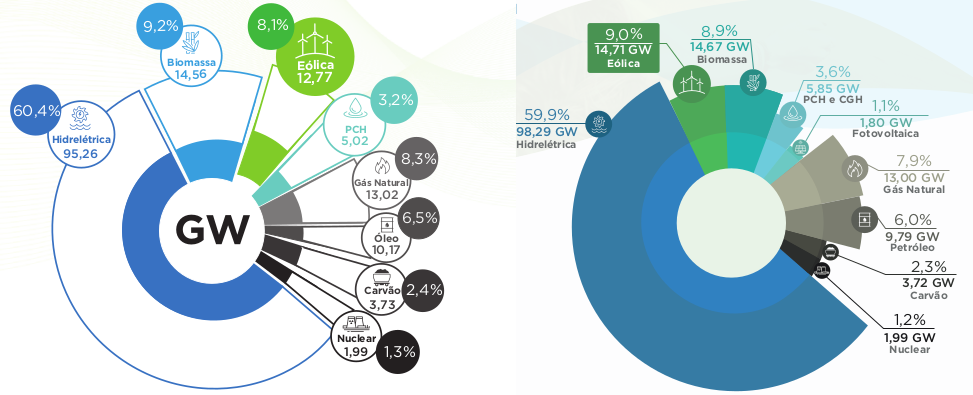
\includegraphics[width=\textwidth]{abe_2017_2018}
%		\caption{Comparação entre a composição da matriz energética brasileira no ano de 2017 (esquerda) e no ano de 2018 (direita)}
	\end{figure}
\end{frame}

\begin{frame}
	\frametitle{Ranking de capacidade eólica instalada acumulada}
	\begin{figure}
		\centering
		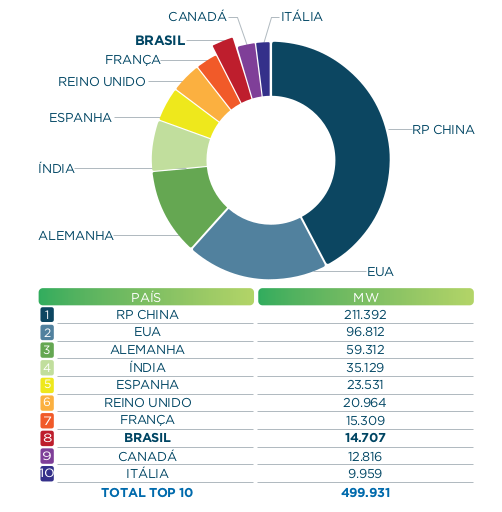
\includegraphics[scale=0.4]{abe_maiores_produtores}
%%		\caption{Ranking de capacidade eólica instalada acumulada}
	\end{figure}
\end{frame}

\begin{frame}
	\frametitle{Evolução da capacidade instalada de parques eólicos no Brasil}
	\begin{figure}
		\centering
		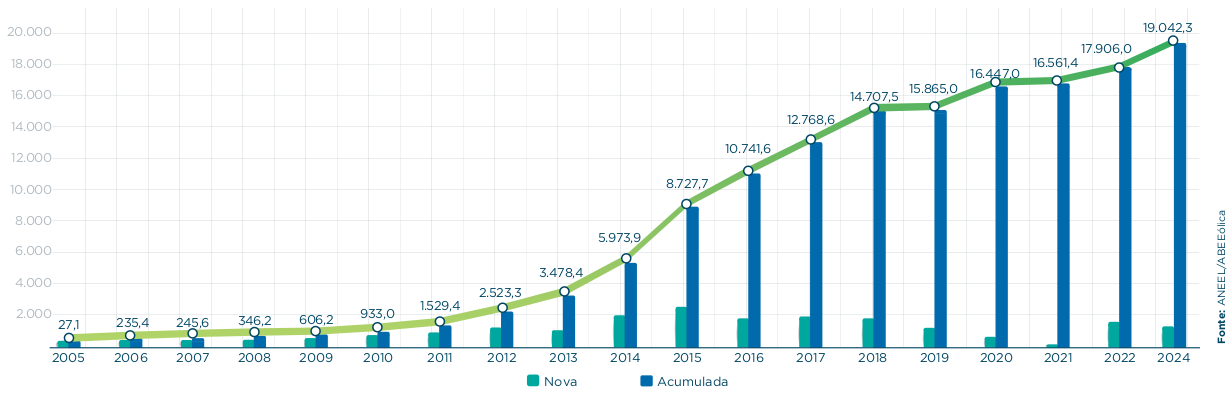
\includegraphics[width=\textwidth]{abe_evolucao_capacidade_instalada}
%%		\caption{Evolução da capacidade instalada de parques eólicos no Brasil}
	\end{figure}
\end{frame}



\begin{frame}
	\frametitle{Variáveis estocásticas}

	O arcabouço teórico desenvolvido para estudar séries financeiras pode ser aplicado no estudo de outras séries estocásticas.

	\begin{figure}
		\centering
		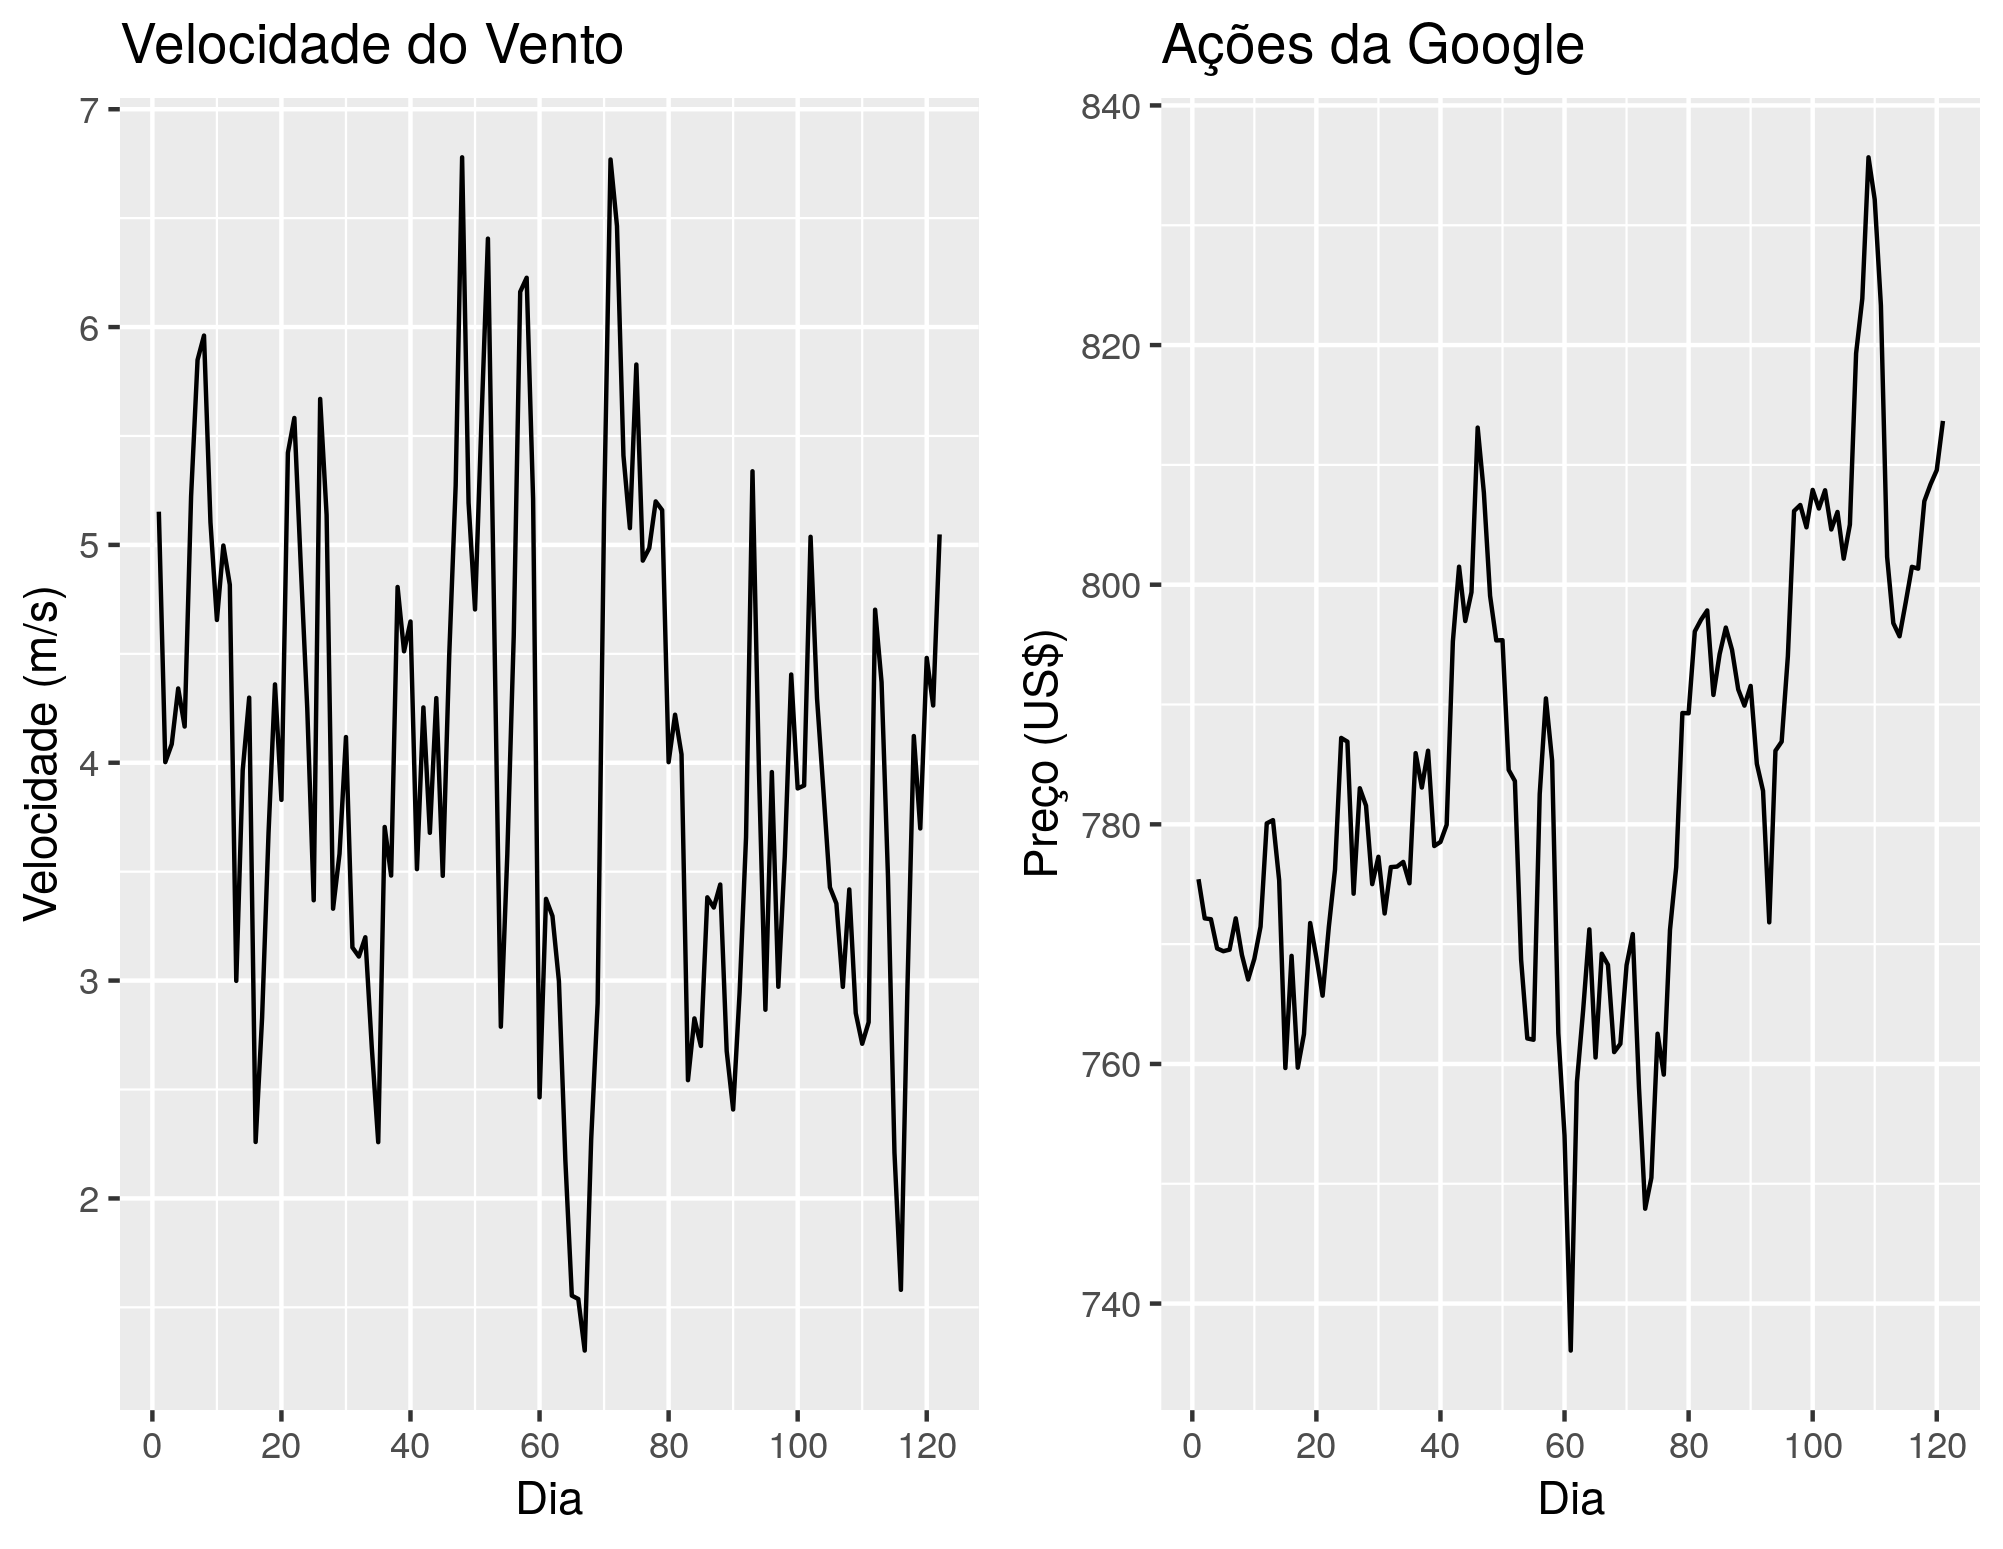
\includegraphics[scale=0.5]{wind_money}
%%		\caption{era5.}
	\end{figure}
\end{frame}

\section{Estudo de Caso}

\subsection{Caracterização da região}

\begin{frame}
	\frametitle{Variação da elevação na direção preferencial de escoamento do vento.}
	\begin{figure}
		\centering
		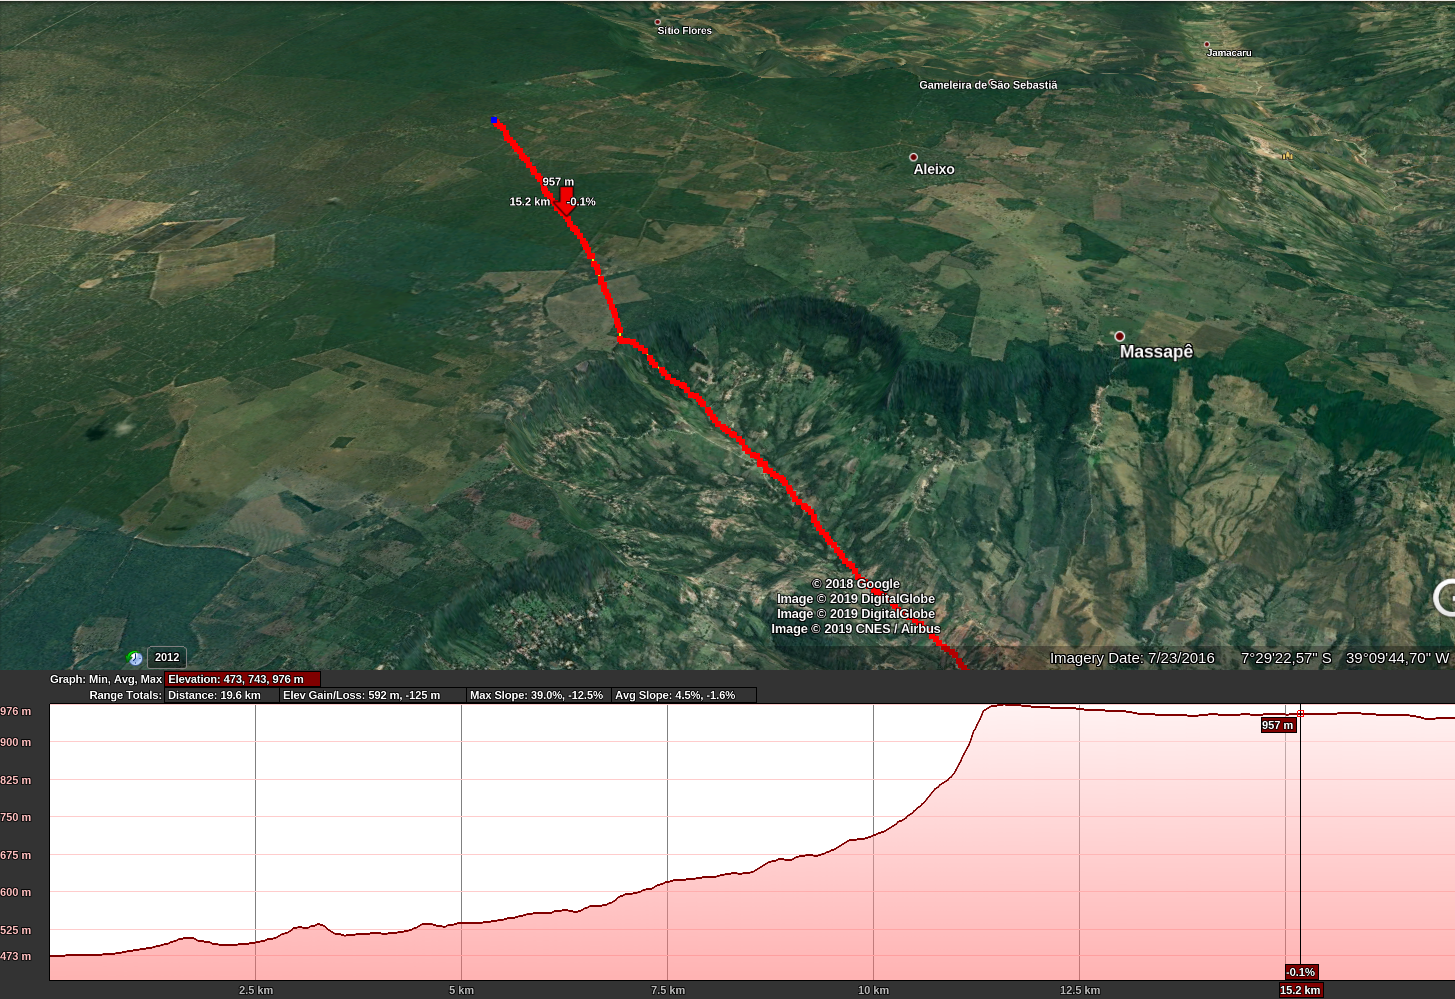
\includegraphics[scale=0.19]{elevation2}
%%		\caption{Chapada}
	\end{figure}
\end{frame}

\begin{frame}
	\frametitle{Topografia}
	\begin{figure}
		\centering
		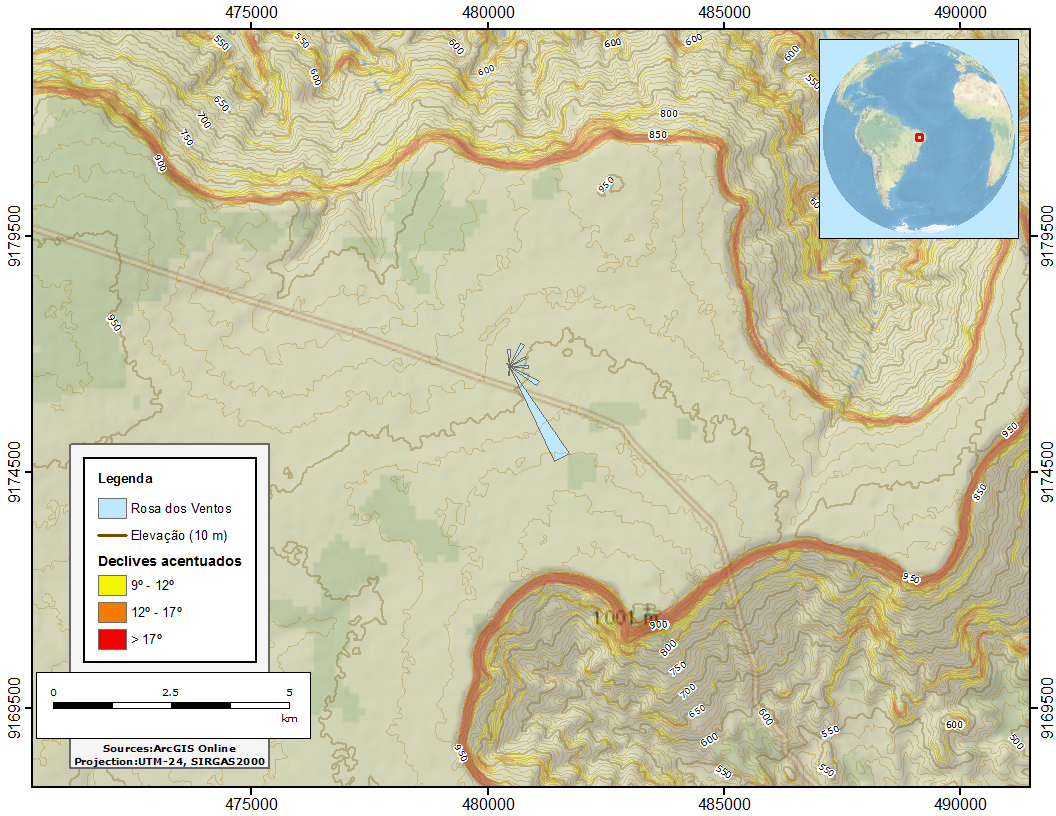
\includegraphics[scale=0.35]{arcmap}
%%		\caption{Variação da elevação na direção preferencial de escoamento do vento.}
	\end{figure}
\end{frame}

\subsection{A série temporal modelo}

\begin{frame}
	\frametitle{ERA 5}
	\begin{figure}
		\centering
		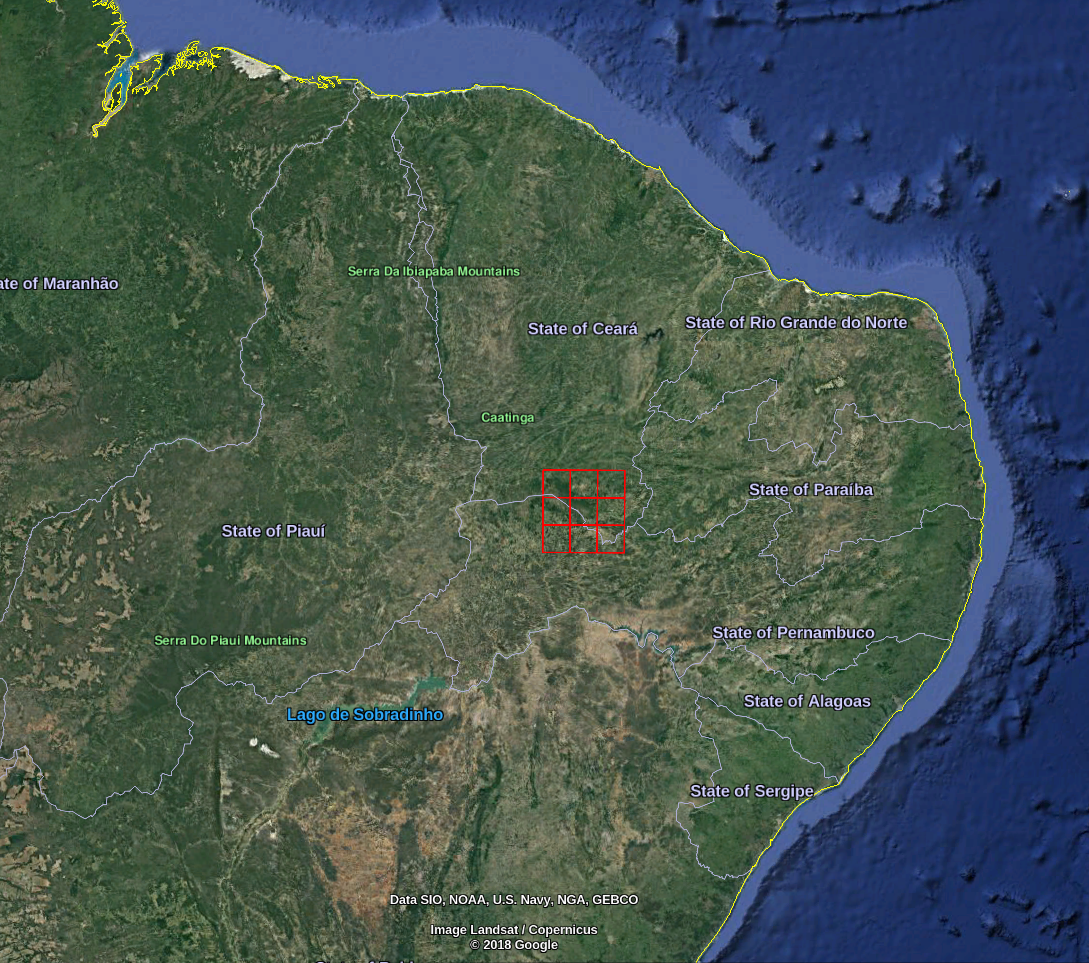
\includegraphics[scale=0.9]{era5nodes}
%%		\caption{Alguns nós da série ERA 5 ao sul do Ceará, Brasil.\newline Google earth V 7.3.2.5776. (14 de Dezembro, 2015). Rio Grande do Sul, Brasil.}
	\end{figure}
\end{frame}

\begin{frame}
	\frametitle{ERA 5}
	\begin{itemize}
		\item<1-> Medições por satélite
		\item<2-> For correlação com torres no solo
		\item<3-> Aperfeiçoada em relação a ERA-Interim e MERRA2
		\item<4-> Altura de medição a 100 m
		\item<5-> Dados horários
		\item<6-> Resolução espacial de 30 km
		\item<7-> 20 anos de dados
	\end{itemize}
\end{frame}

\subsection{Caracterização dos dados}

\begin{frame}
	\frametitle{Velocidade do vento registrada por satélite na região de interesse nos anos de 2017 e 2018}
	\begin{figure}
		\centering
		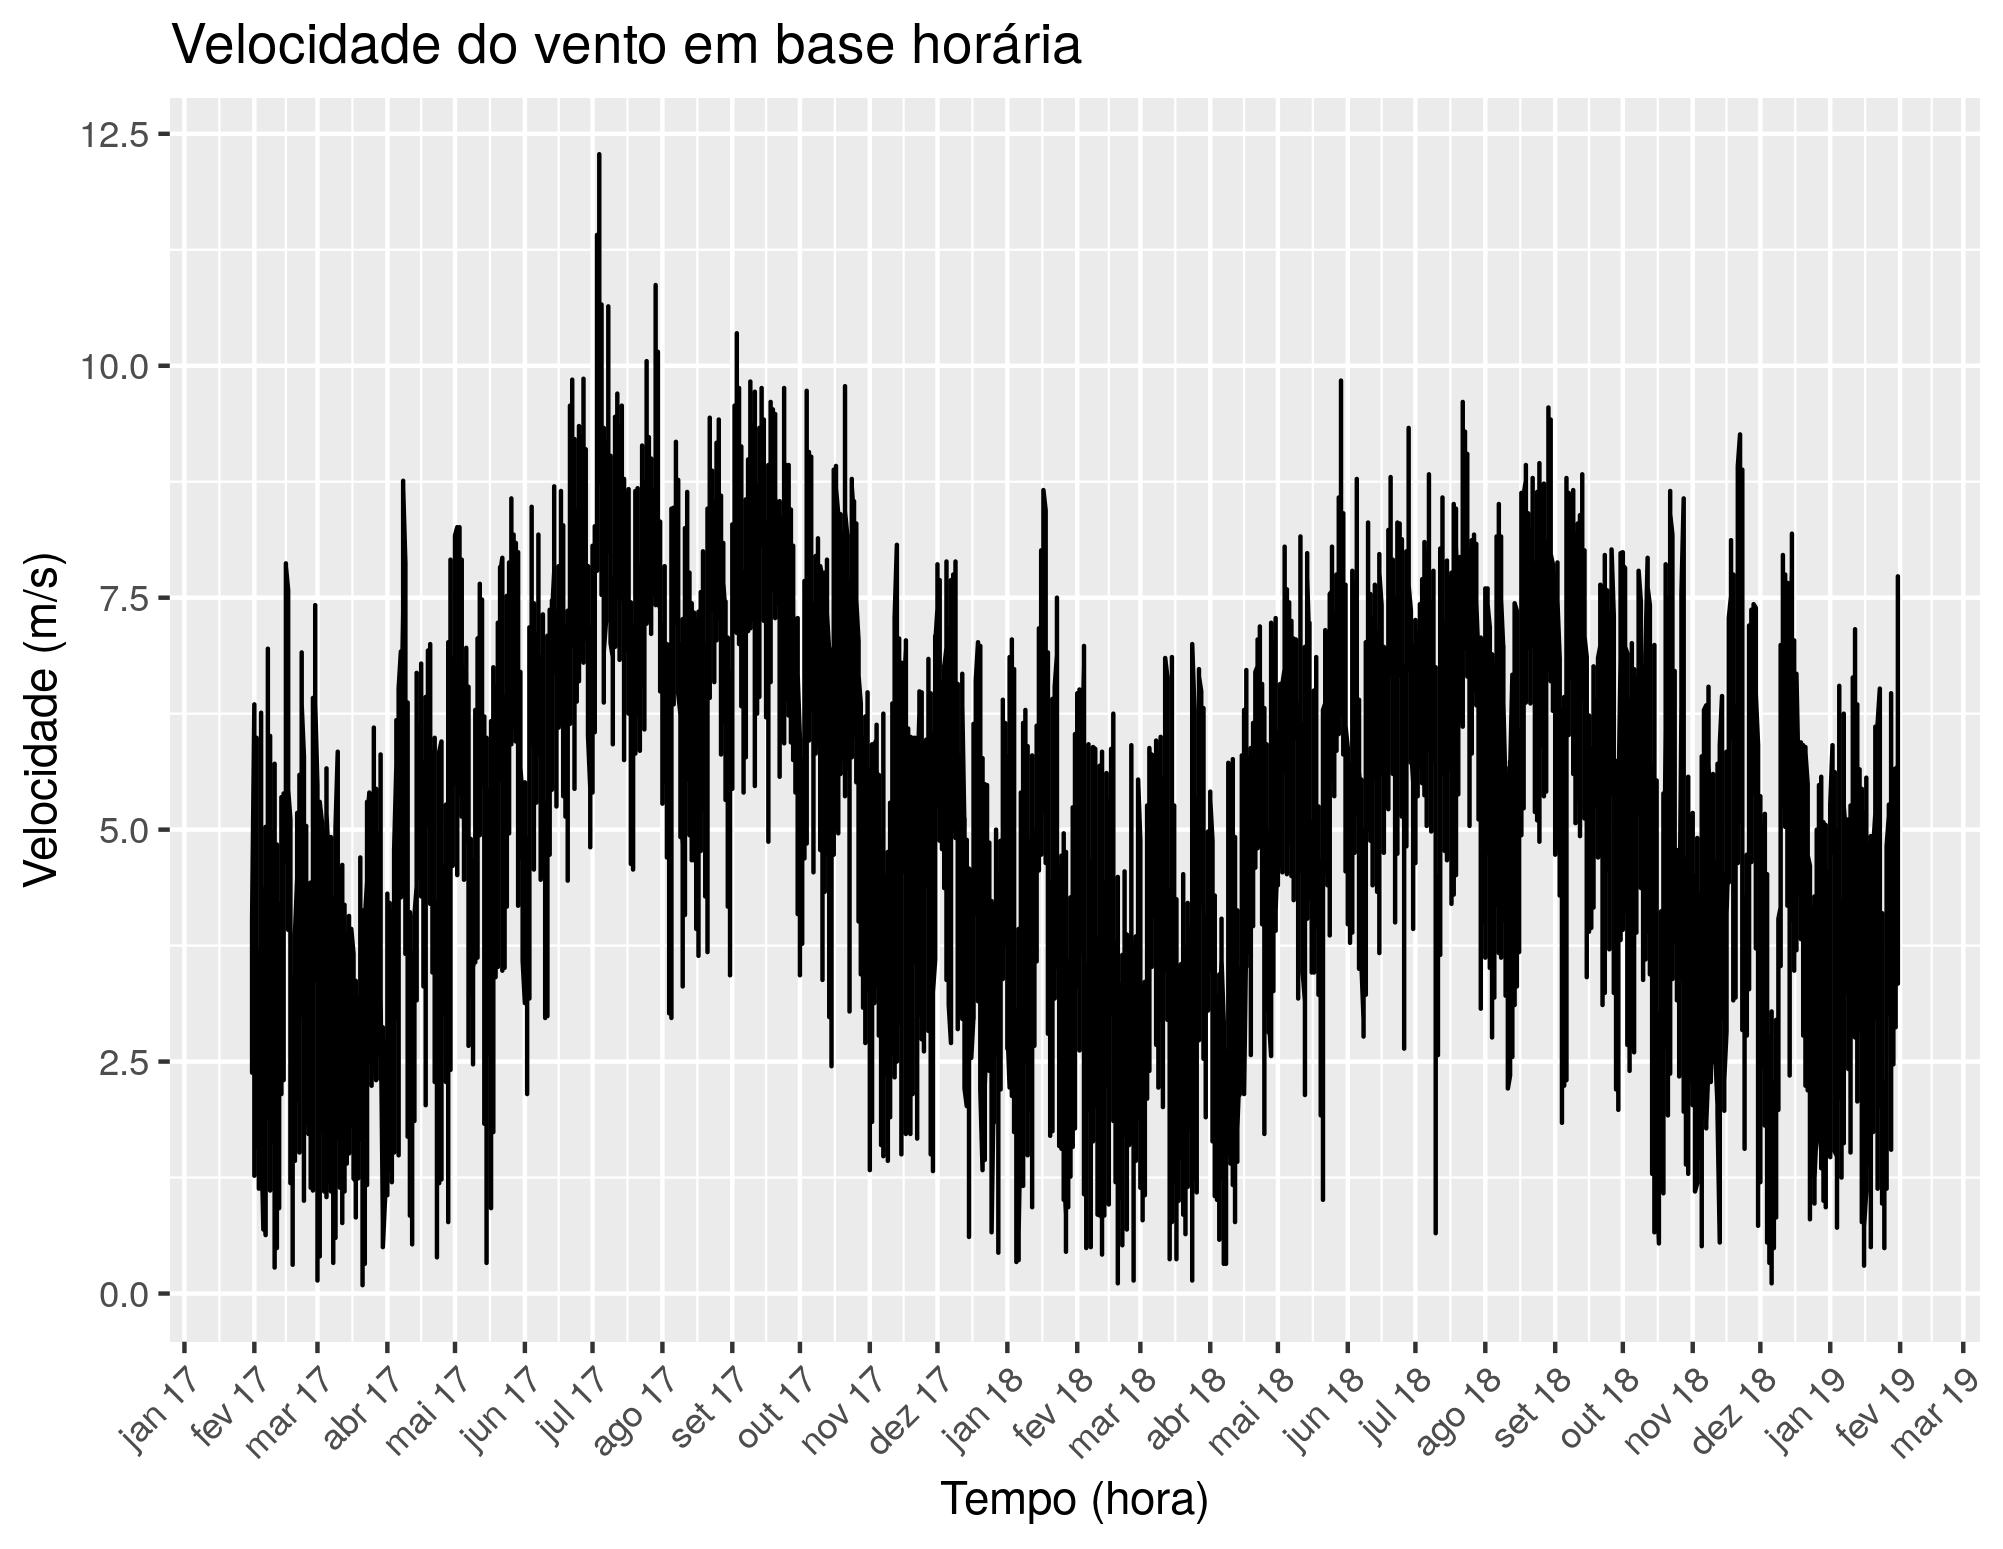
\includegraphics[scale=0.55]{entire_series_hourly_basis.png}
%%		\caption{Velocidade do vento registrada por satélite na região de interesse nos anos de 2017 e 2018}
	\end{figure}
\end{frame}

\begin{frame}
	\frametitle{Histograma de velocidades do nó noroeste da série de dados modelo.}
	\begin{figure}
		\centering
		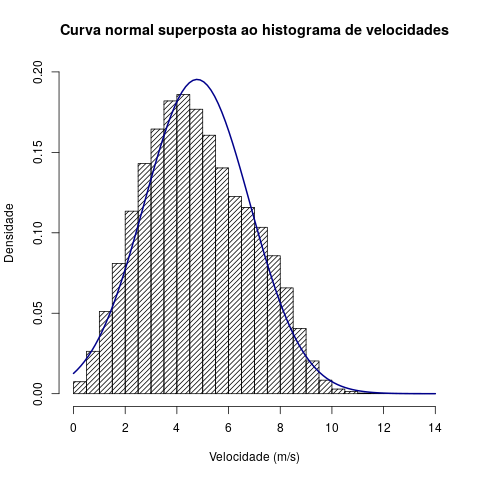
\includegraphics[scale=0.43]{normal_overlay}
%%		\caption{Histograma de velocidades do nó noroeste da série de dados modelo.}
	\end{figure}
\end{frame}

\begin{frame}
	\frametitle{Distribuição de cauda longa}
	\begin{figure}
		\centering
		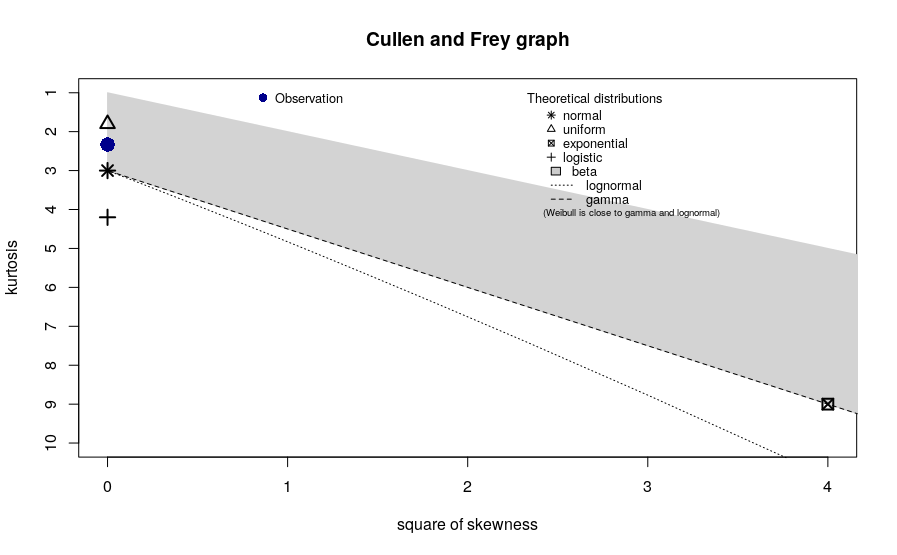
\includegraphics[scale=0.5]{cullen}
%%		\caption{Gráfico de Cullen e Frey para os dados do nó noroeste da série de dados modelo.}
	\end{figure}
\end{frame}

\begin{frame}
	\frametitle{Direção: rosa dos ventos de longo prazo}
	\begin{figure}
		\centering
		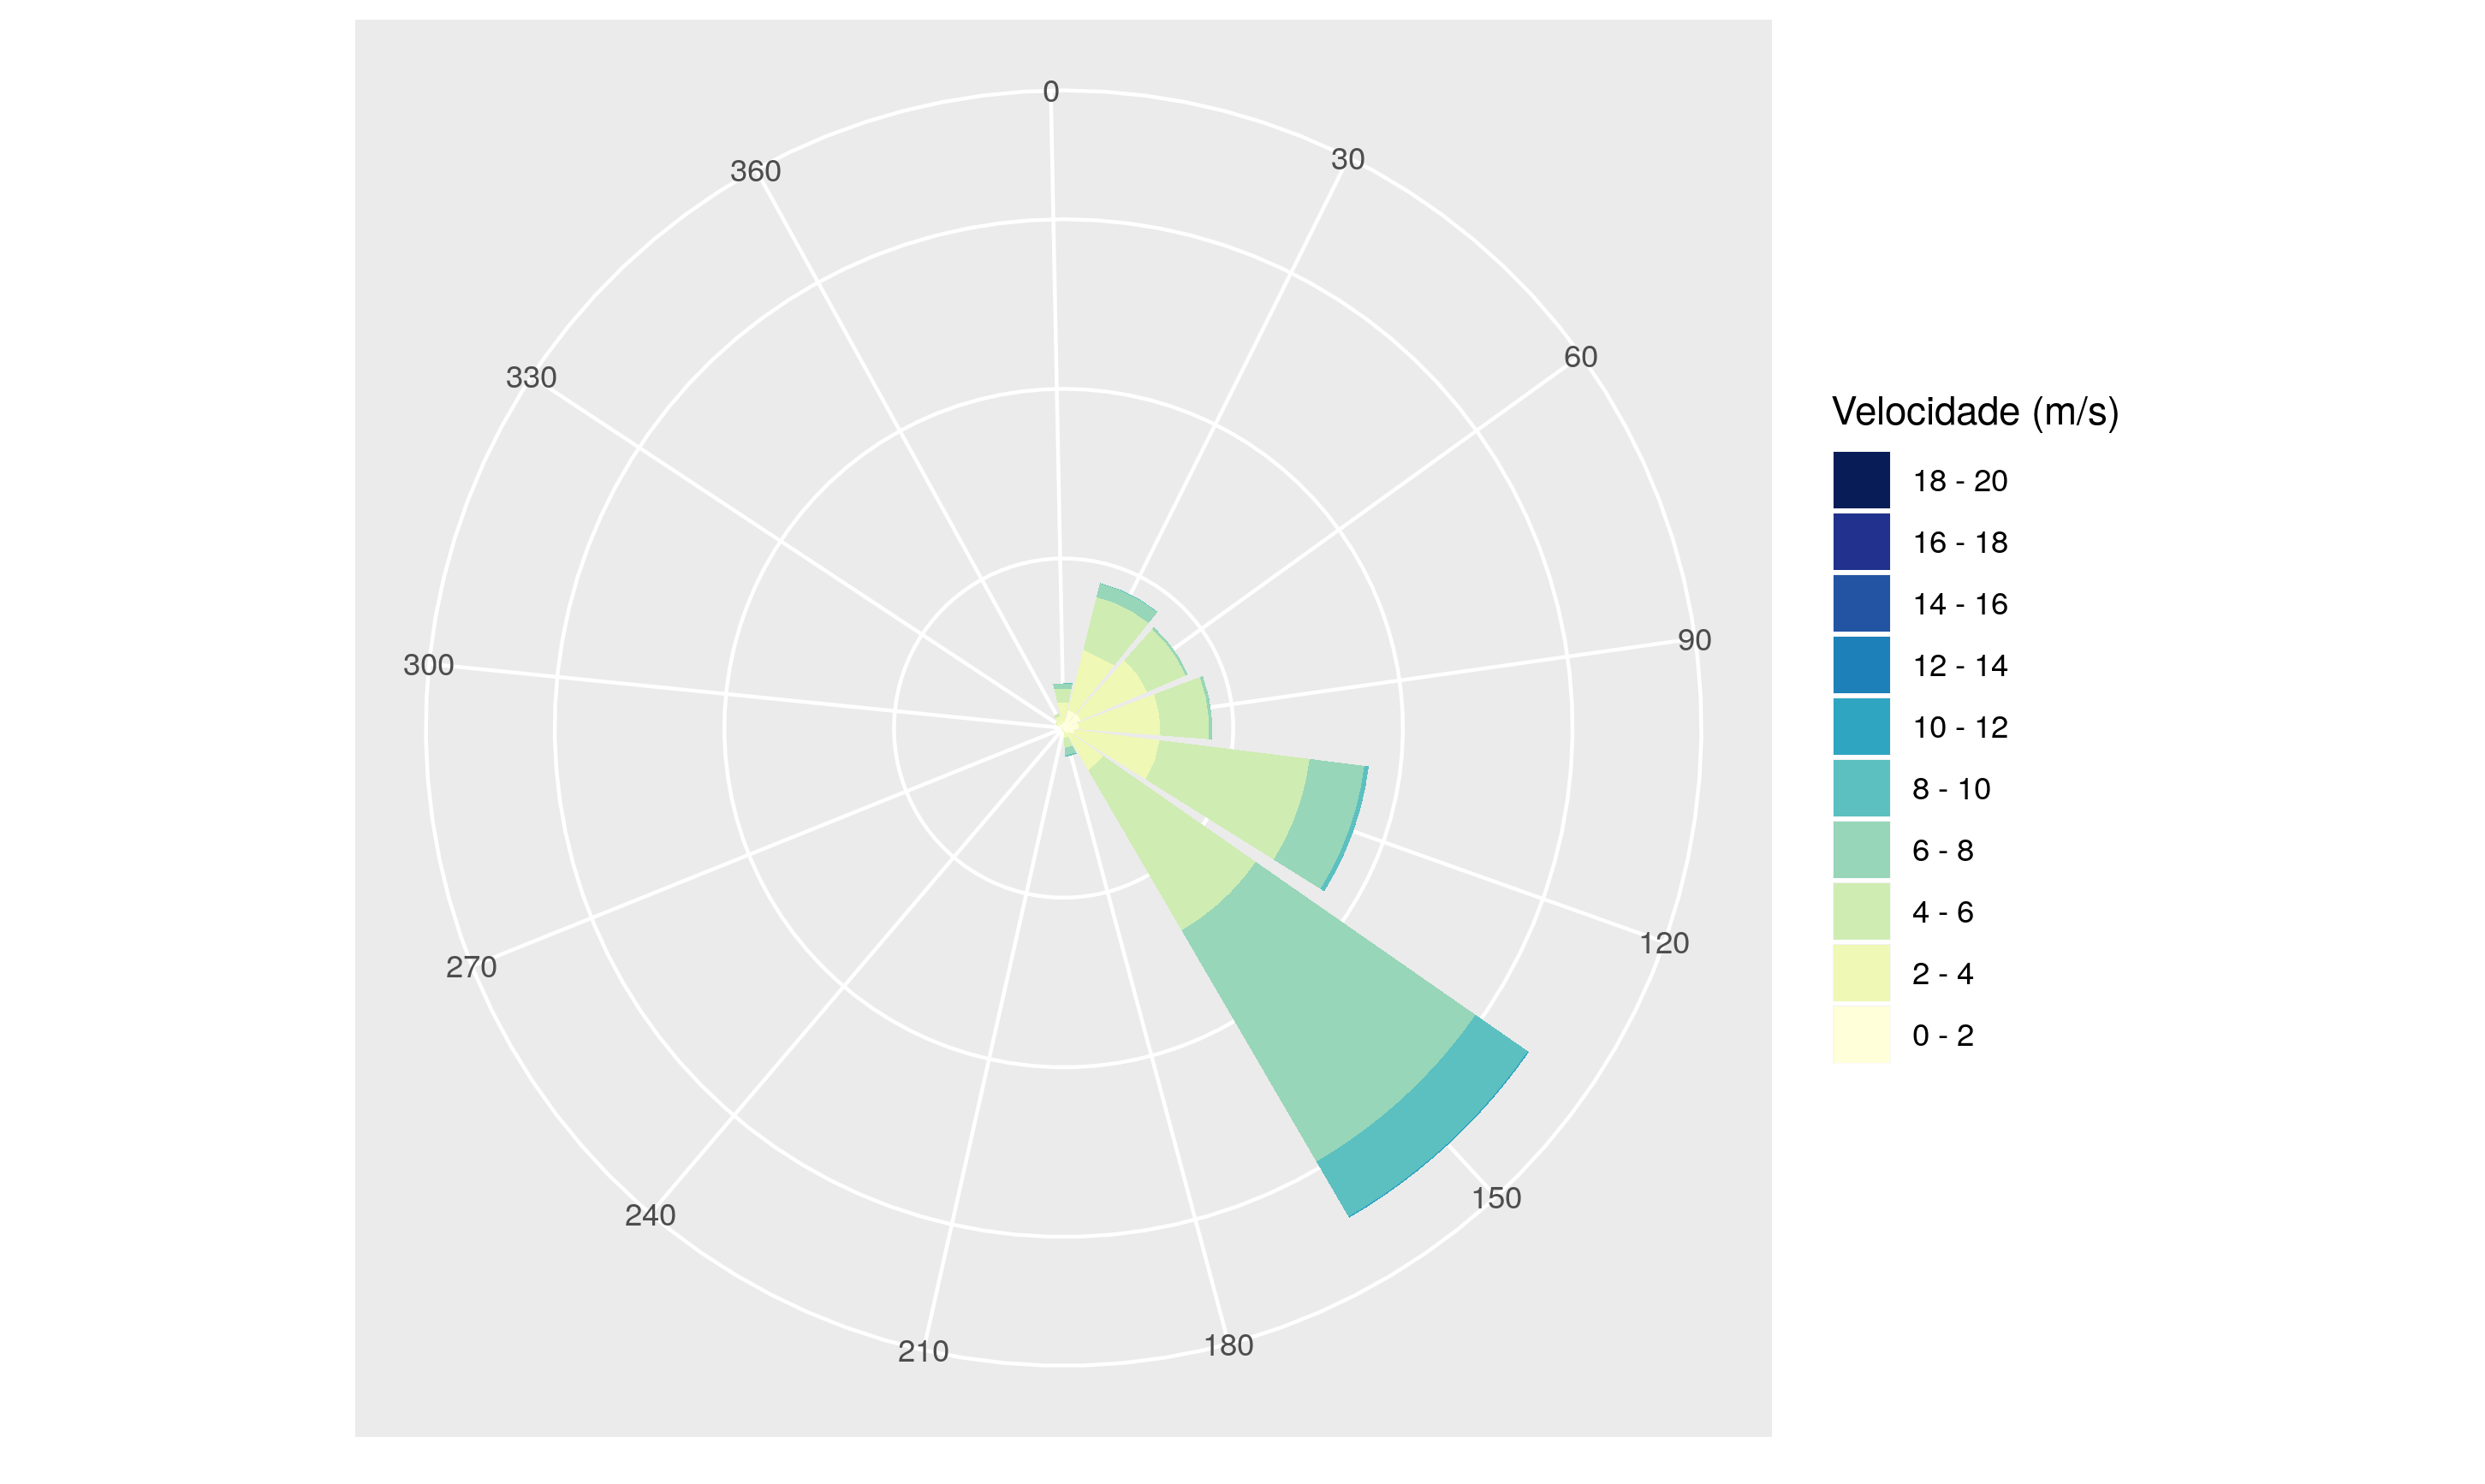
\includegraphics[scale=0.6]{windrose}
%%		\caption{Rosa dos ventos}
	\end{figure}
\end{frame}

\begin{frame}
	\frametitle{Sazonalidade}
	\begin{figure}
		\centering
		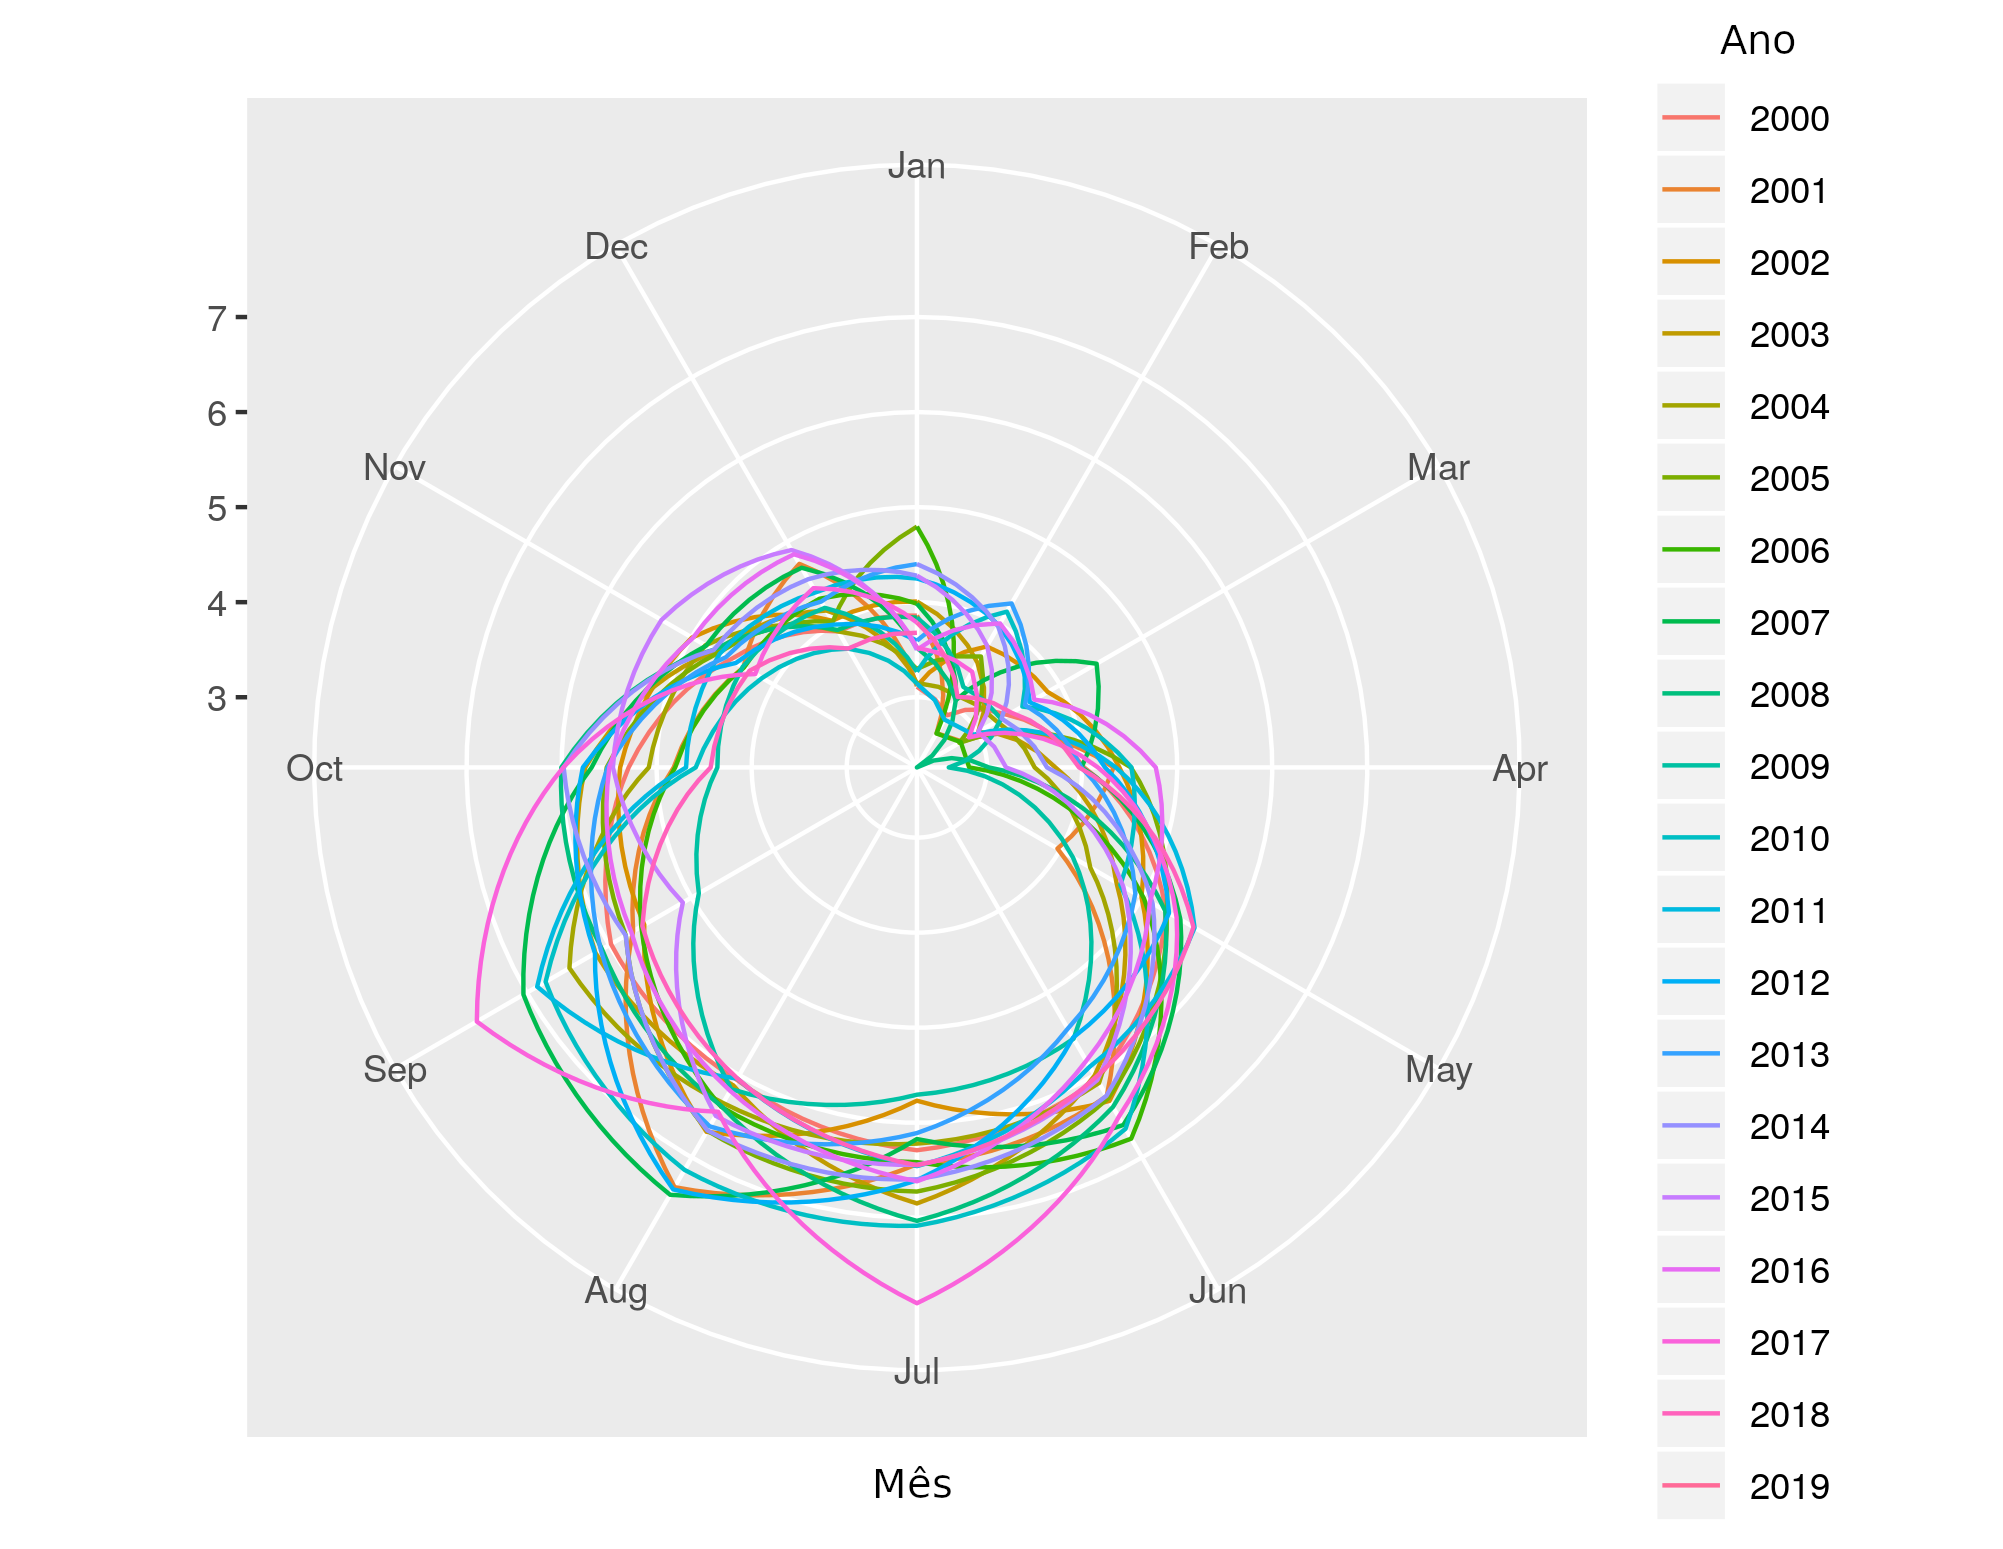
\includegraphics[scale=0.6]{season_plot_polar}
%%		\caption{Chapada}
	\end{figure}
\end{frame}

\section{Implementação}

\subsection{Box-Jenkins}

\begin{frame}
	\frametitle{ARIMA}
		
	\begin{block}{AR}			
		\begin{equation*}
			y^{'}_{t} = c + \phi_{1}y^{'}_{t-1} + \dots + \phi_{p}y^{'}_{t-p}
		\end{equation*}
	\end{block}
	
	\pause	
	
	\begin{block}{MA}
		\begin{equation*}
			y^{'}_{t} = \theta_{1}\varepsilon_{t-1} + \dots + \theta_{q}\varepsilon_{t-q} + \varepsilon_{t}
		\end{equation*}
	\end{block}
	
	\pause	
		
	\begin{block}{ARIMA}
		\begin{equation*}
			y^{'}_{t} = c + \phi_{1}y^{'}_{t-1} + \dots + \phi_{p}y^{'}_{t-p} + \theta_{1}\varepsilon_{t-1} + \dots + \theta_{q}\varepsilon_{t-q} + \varepsilon_{t}
		\end{equation*}
	\end{block}		
	
	Onde $y^{'}_{t}$ representa a série de entrada $y_{t}$ após feitas $d$ diferenciações de modo a torná-la estacionária (parâmetro correspondente ao I em ARIMA)
	
\end{frame}		

\begin{frame}
	\frametitle{Box-Jenkins: como encontrar p,d,q?}

	\begin{enumerate}
		\item<1-> Etapa inicial
		\item<2-> Faça um gráfico dos dados
		\item<3-> Identifique comportamentos atípicos
		\item<4-> Identifique padrões
		\item<5-> A variância parece ser constante ao longo da série?
		\begin{itemize}
			\item<5-> 	Não? Aplique uma transformação Box-Cox para estabilizar a variância até que a série aparente ser estacionária
		\end{itemize}
		\item<6-> 	Analise os gráficos ACF e PACF para identificar prováveis modelos		\item Teste os modelos comparando seus valores de AIC
		\item<7-> Verifique os resíduos por ACF e por Ljung-Box
		\item<8-> Os resíduos se aproximam de ruído branco?
			\begin{itemize}
				\item<8-> Não? Volte para a etapa 6
			\end{itemize}
		\item<9-> Estime parâmetros
		\item<10-> Faça previsões
	\end{enumerate}	
\end{frame}

\begin{frame}
	\frametitle{Análise visual: últimos dois anos da série de vento}
	\begin{figure}
		\centering
		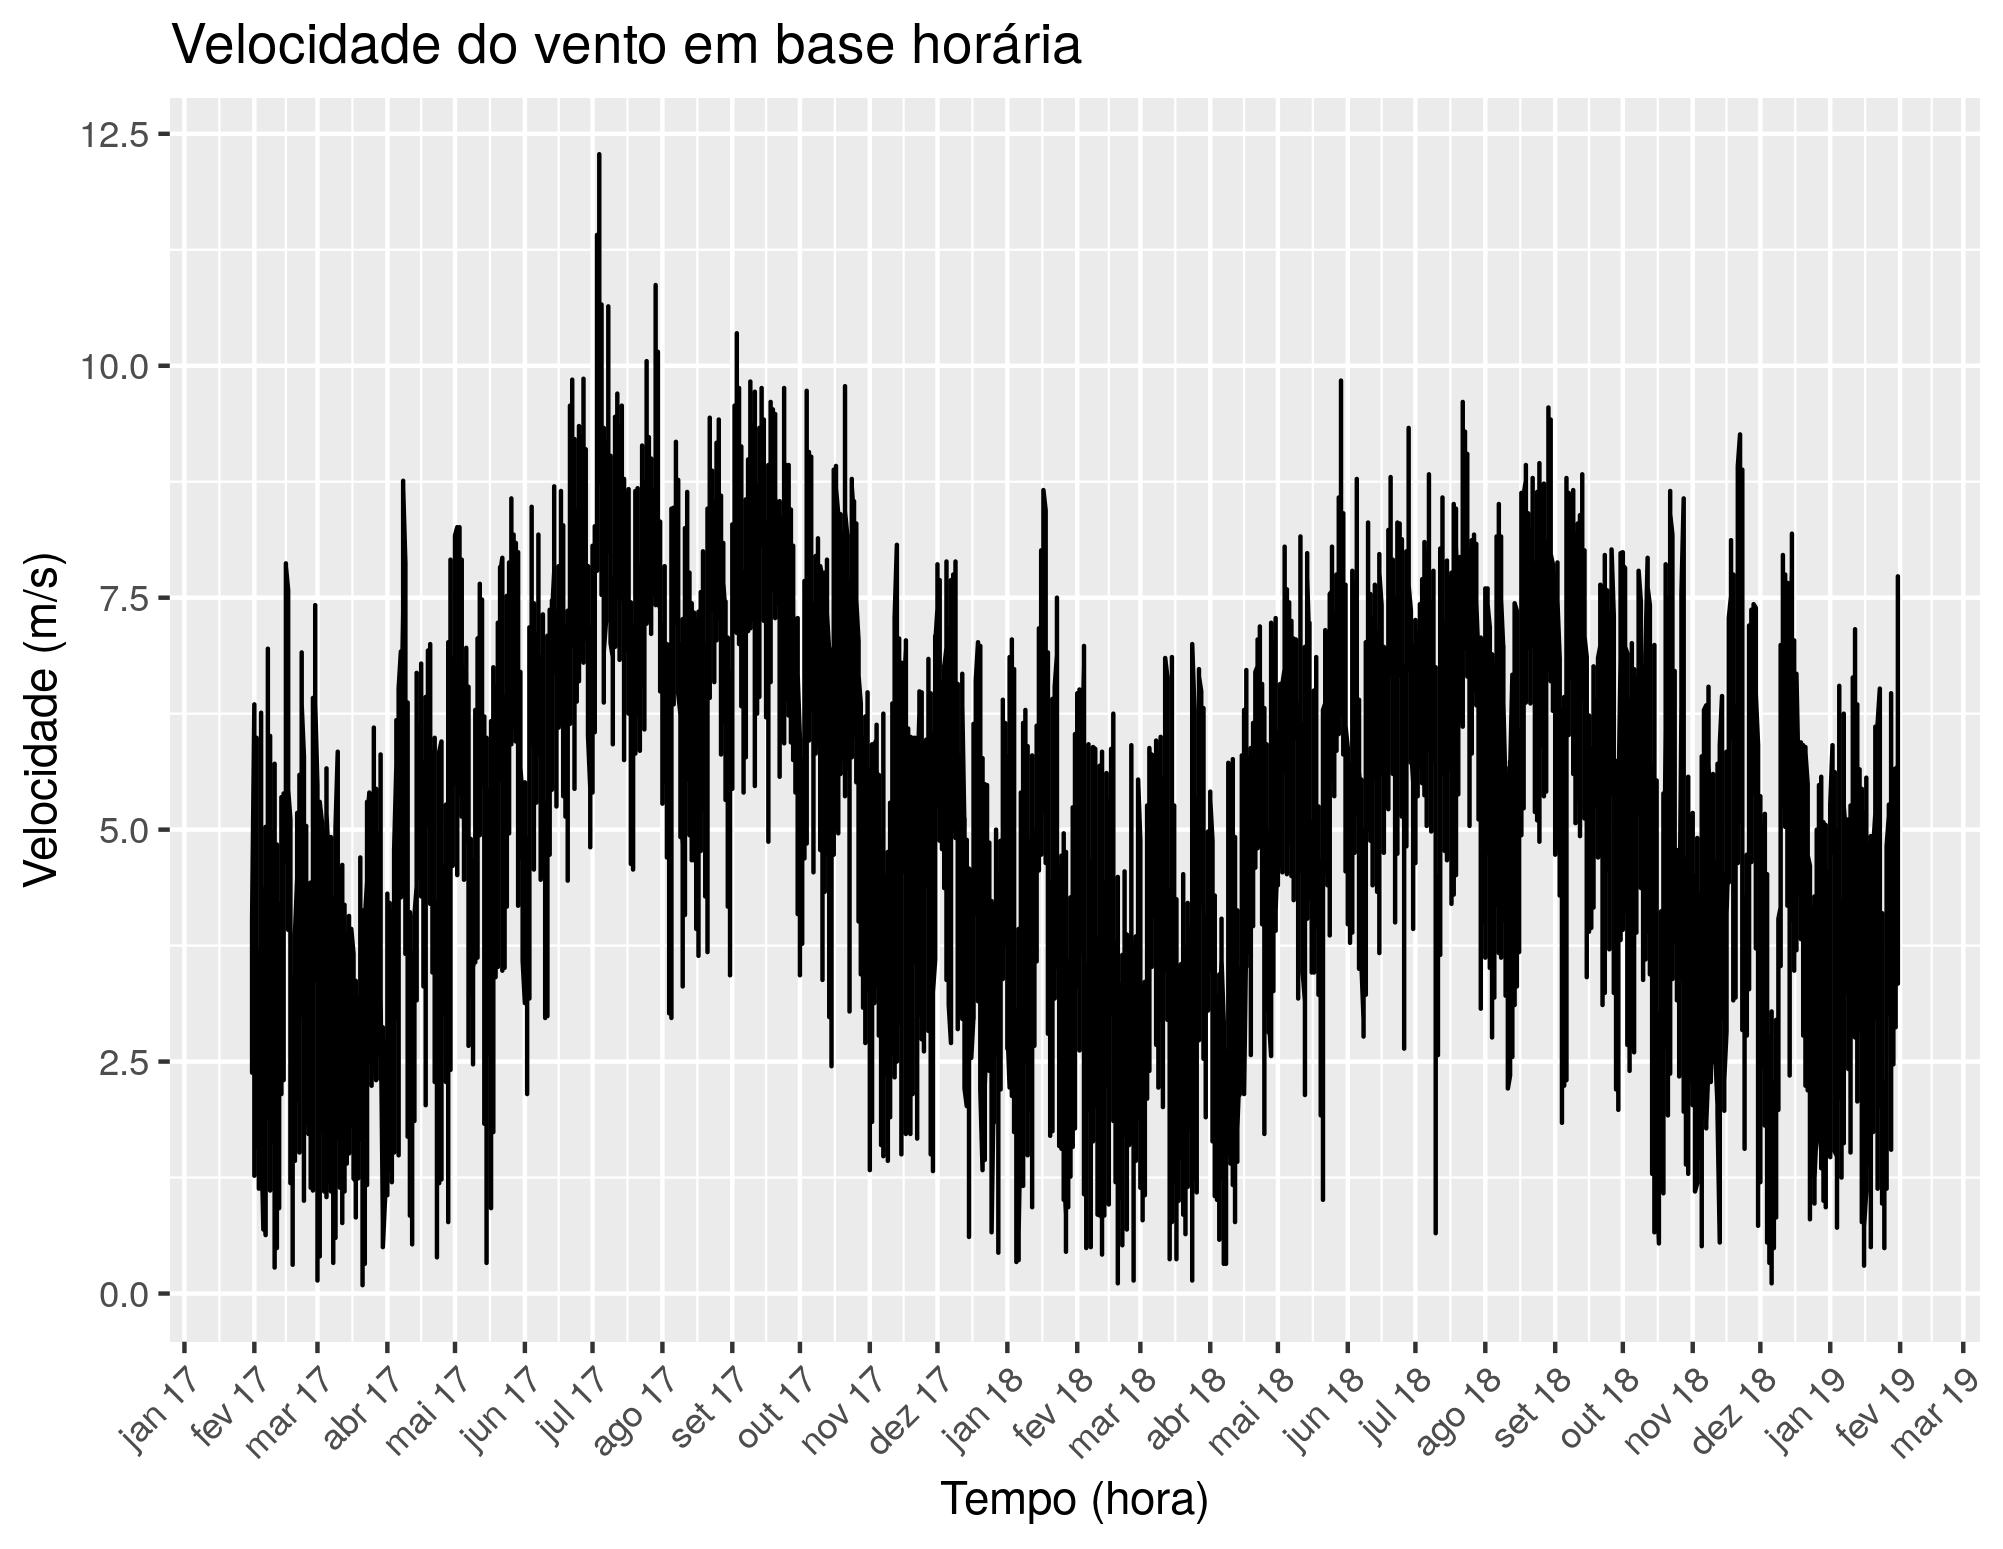
\includegraphics[scale=0.6]{entire_series_hourly_basis}
%%		\caption{Últimos dois anos da série de vento}
	\end{figure}
\end{frame}

\begin{frame}
	\frametitle{Sazonalidade removida por simples diferença}
	\begin{figure}
		\centering
		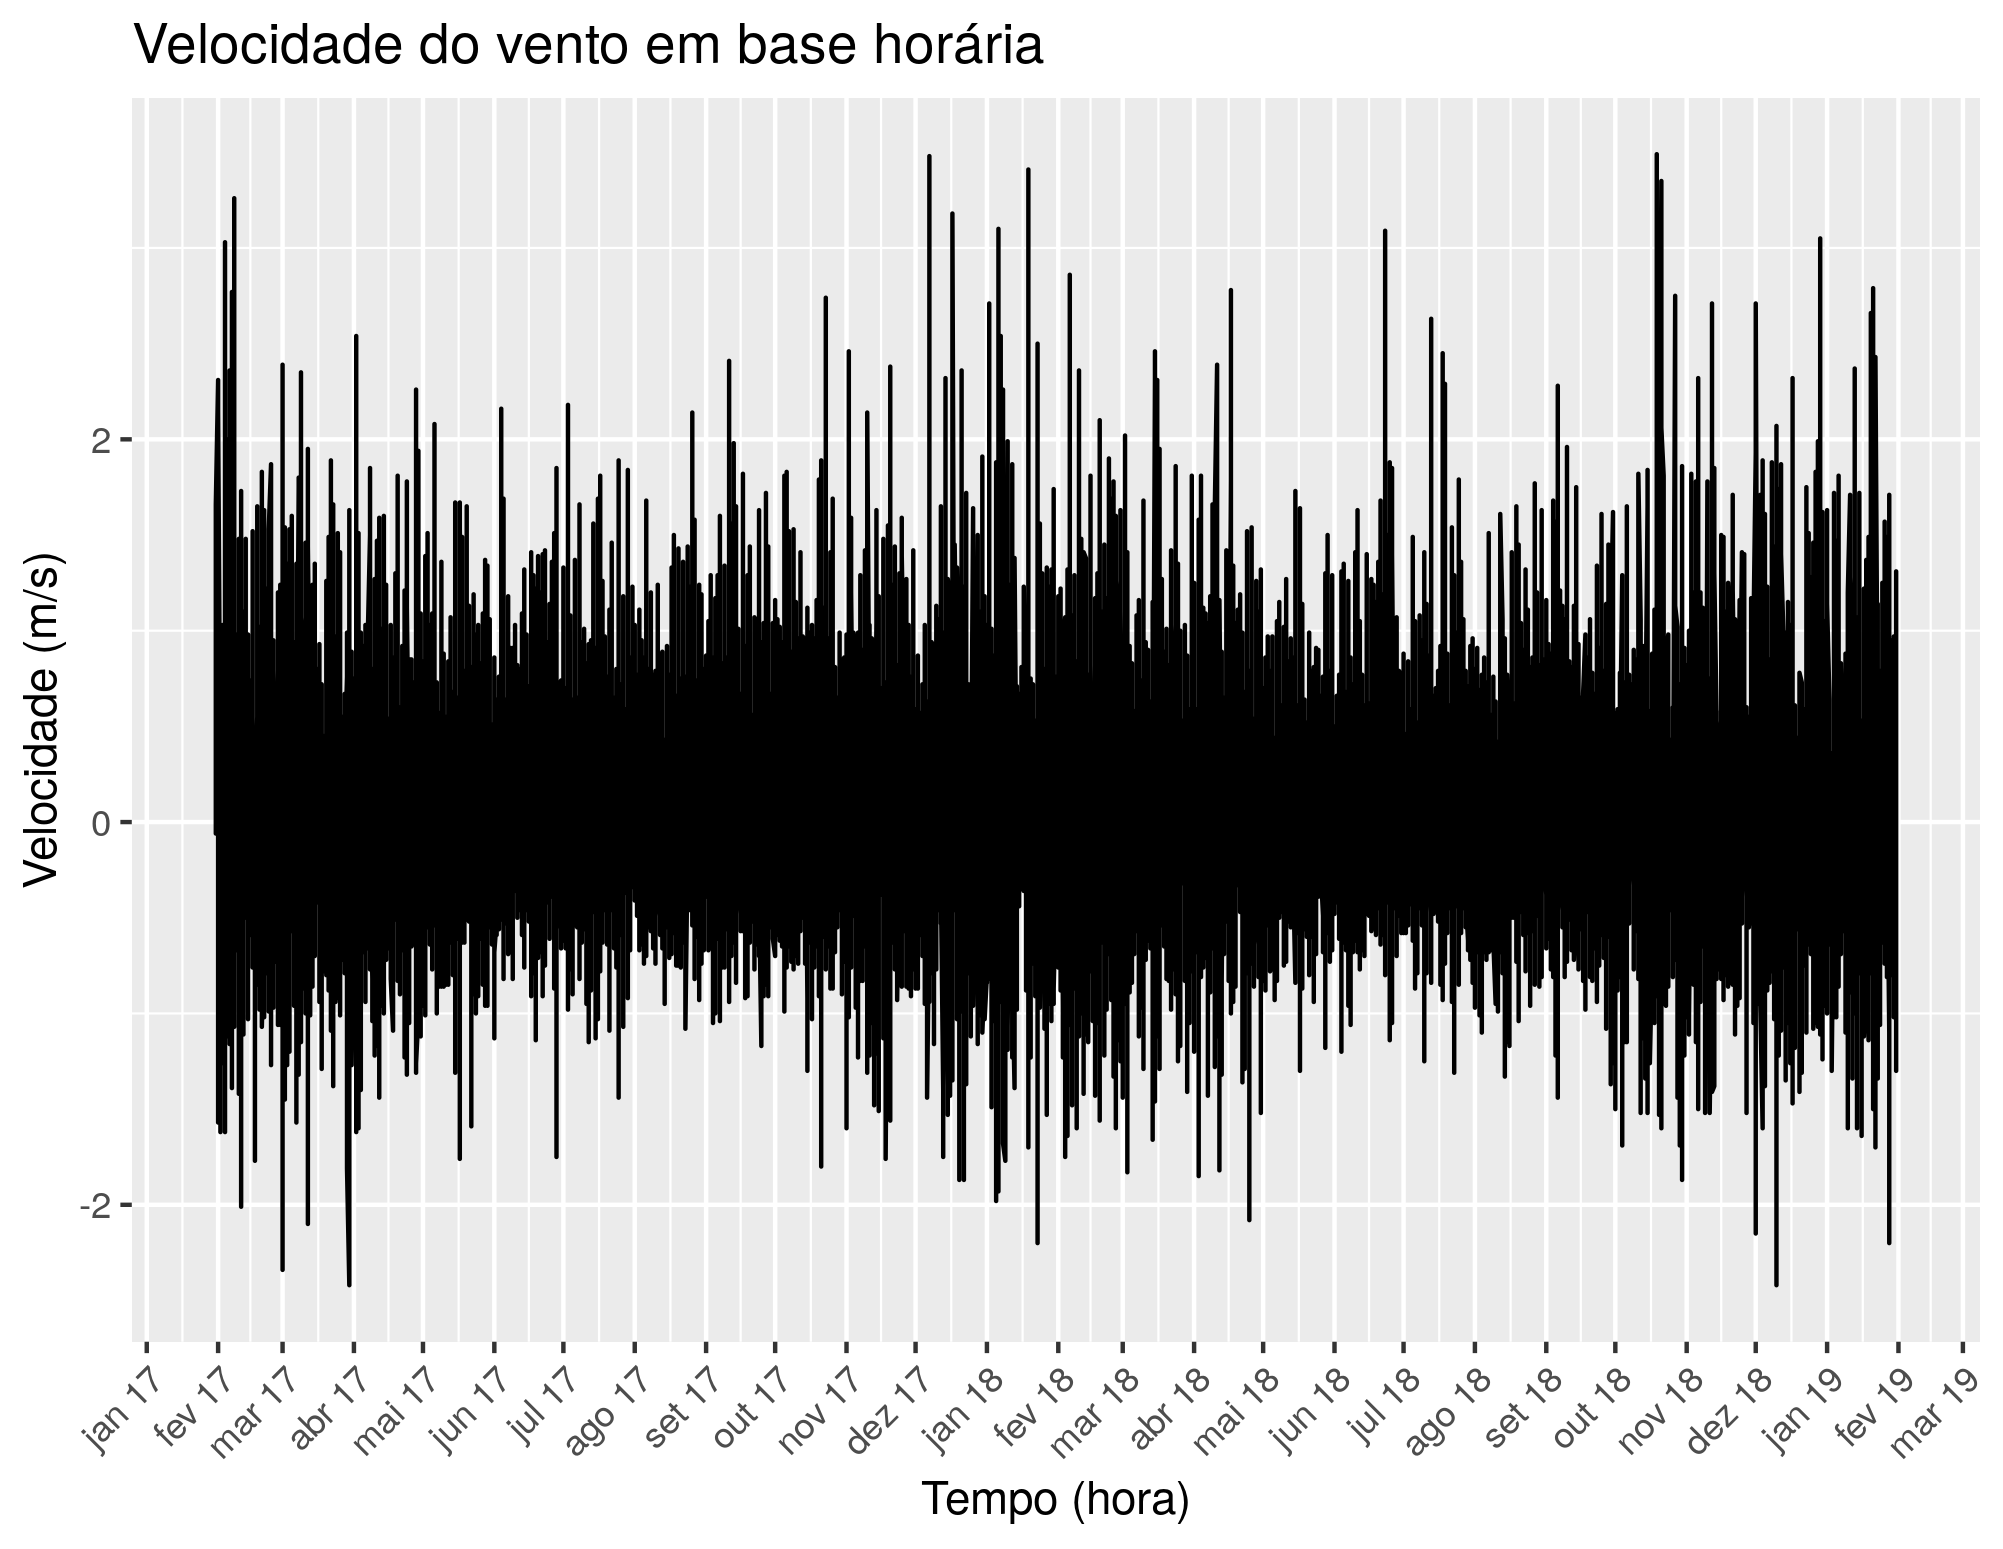
\includegraphics[scale=0.6]{entire_series_hourly_basis_seasonless.png}
%%		\caption{Sazonalidade removida}
	\end{figure}
\end{frame}

\begin{frame}
	\frametitle{Estabilização da variância por meio de uma transformação de Box-Cox}
	\begin{figure}
		\centering
		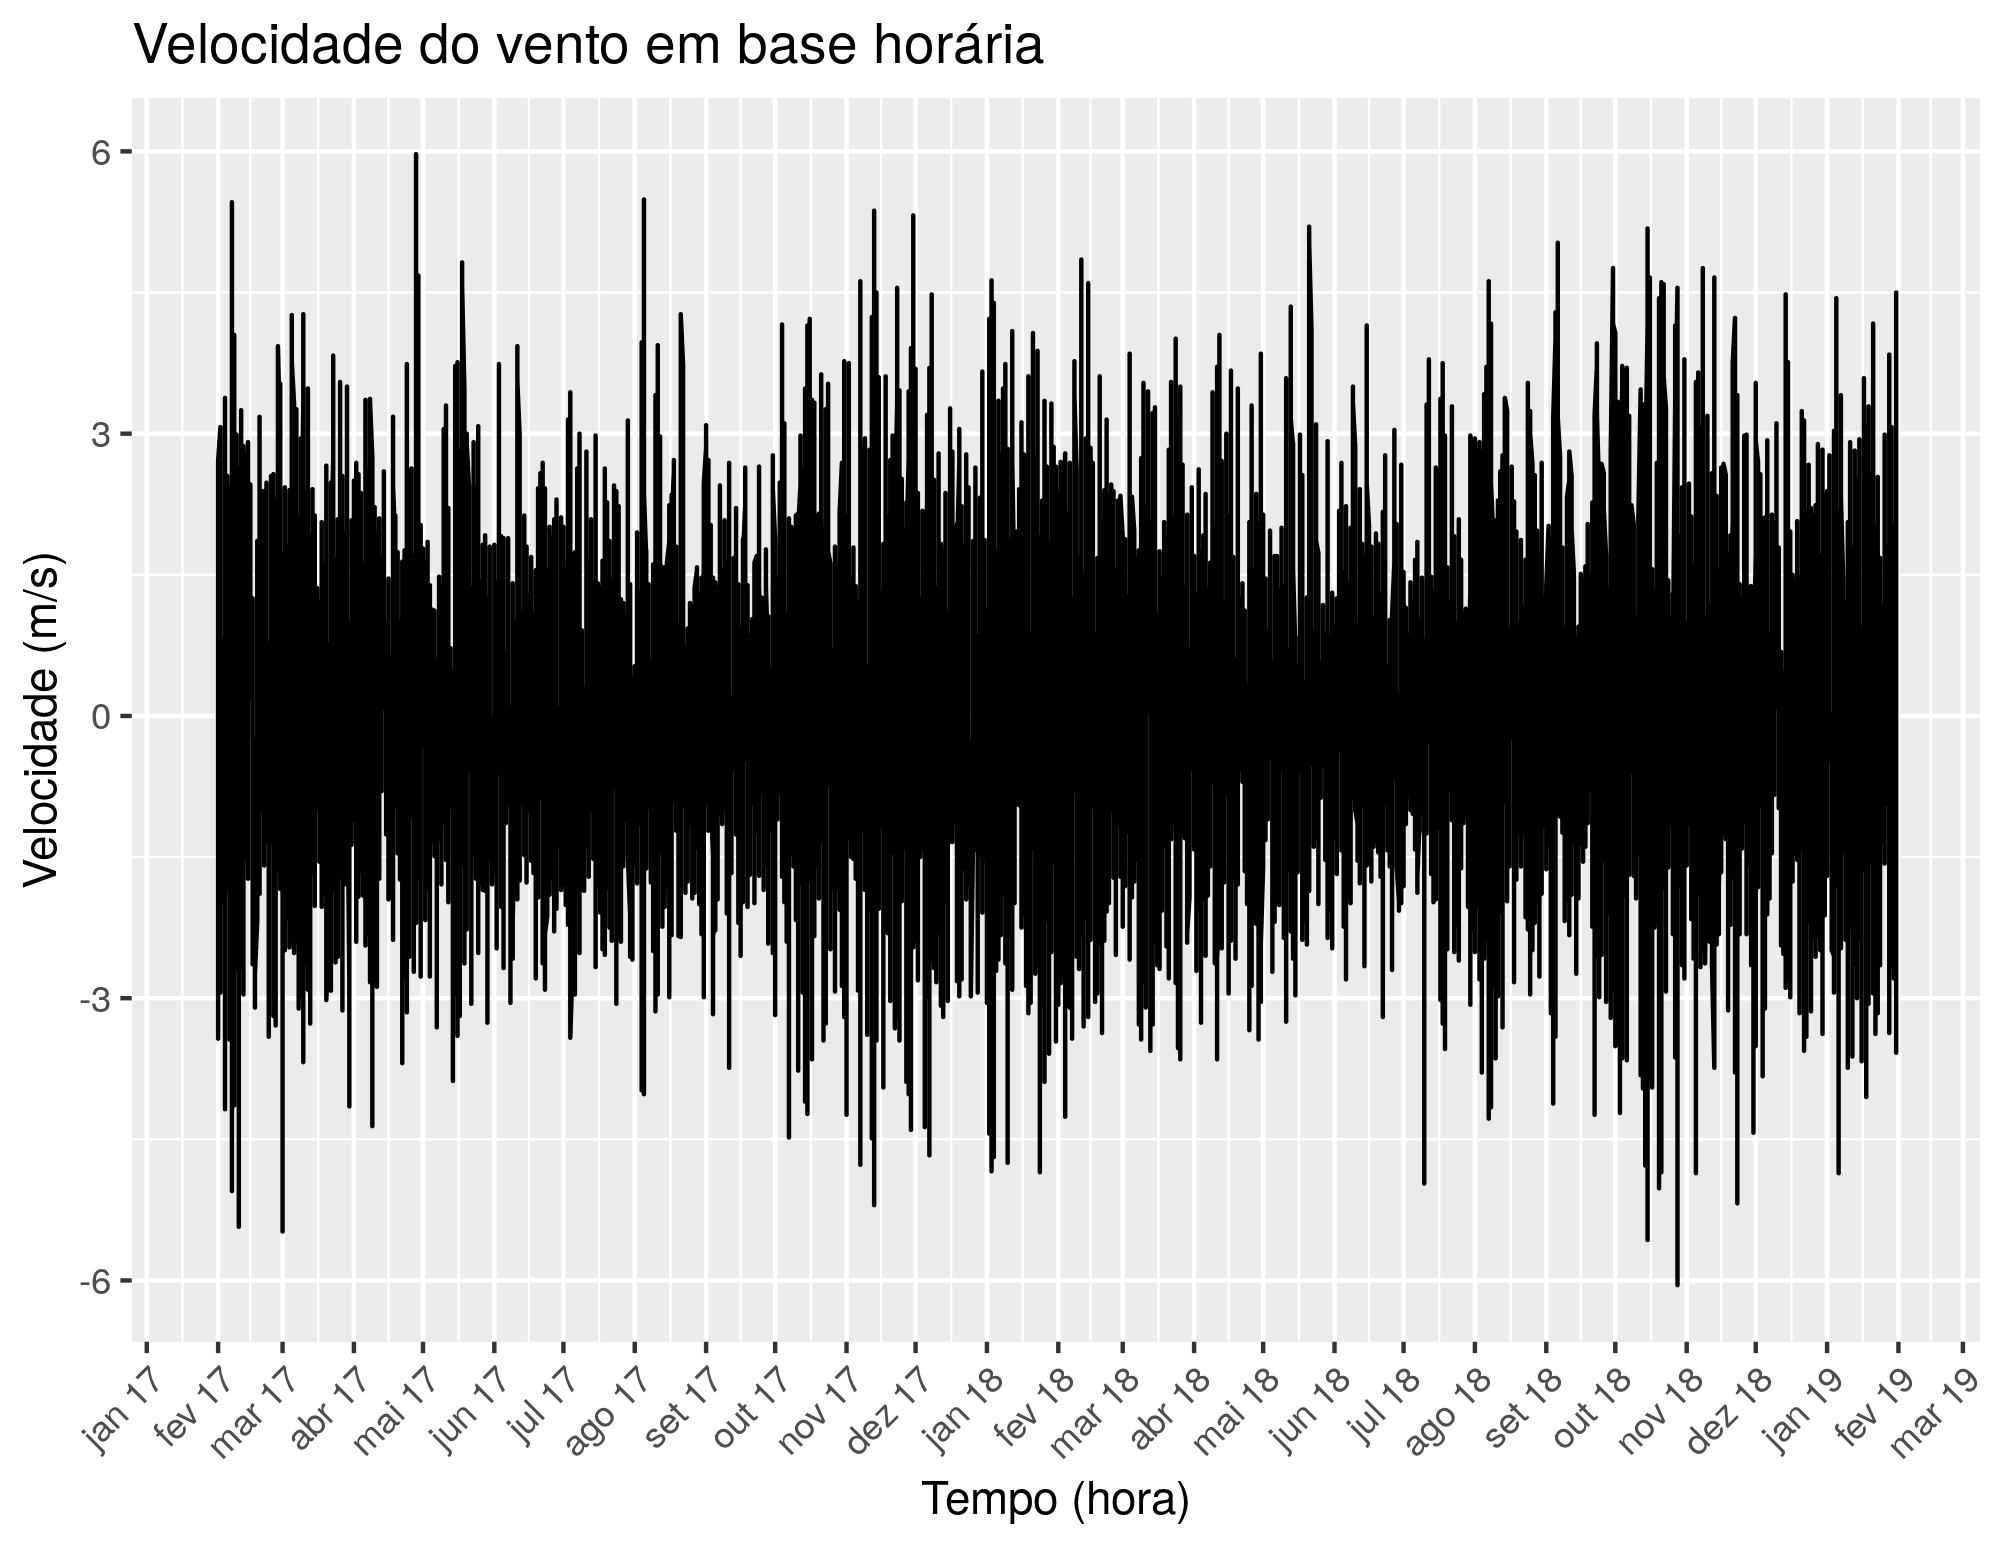
\includegraphics[scale=0.55]{entire_series_hourly_basis_seasonless_boxcox.png}
%%		\caption{Sazonalidade removida por meio de uma transformação de Box-Cox}
	\end{figure}
\end{frame}

\begin{frame}
	\frametitle{PACF: atenuação aparente}
	\begin{figure}
		\centering
		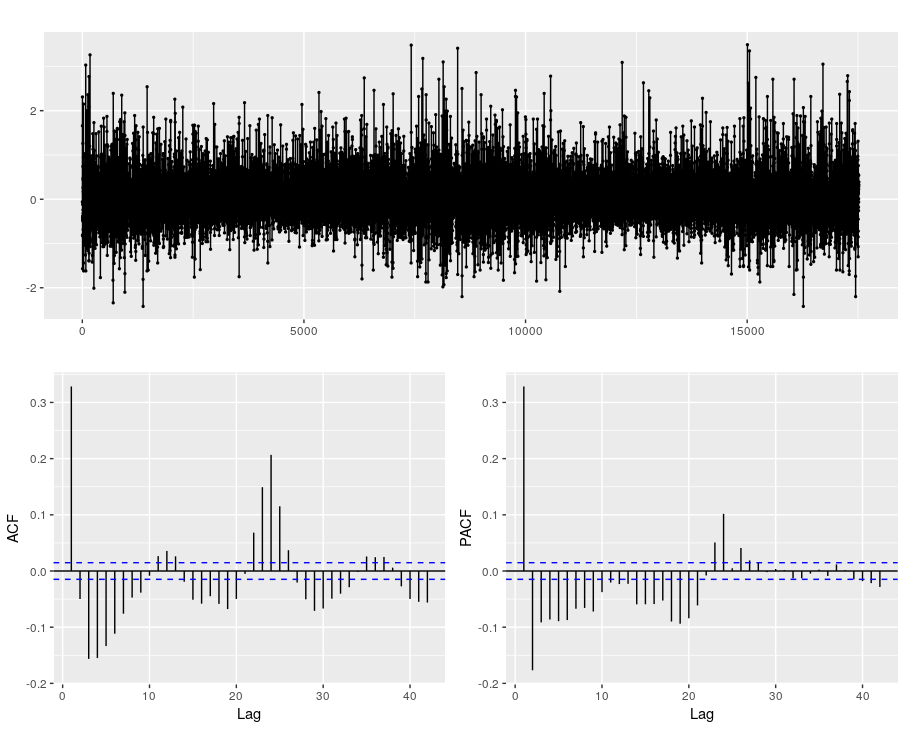
\includegraphics[scale=0.4]{long_memory.png}
%%		\caption{Gráficos da Função de Autocorrelação (ACF) e Função de Autocorrelação Parcial (PACF)}
	\end{figure}
\end{frame}

\begin{frame}
	\frametitle{Memória longa!}
	\begin{figure}
		\centering
		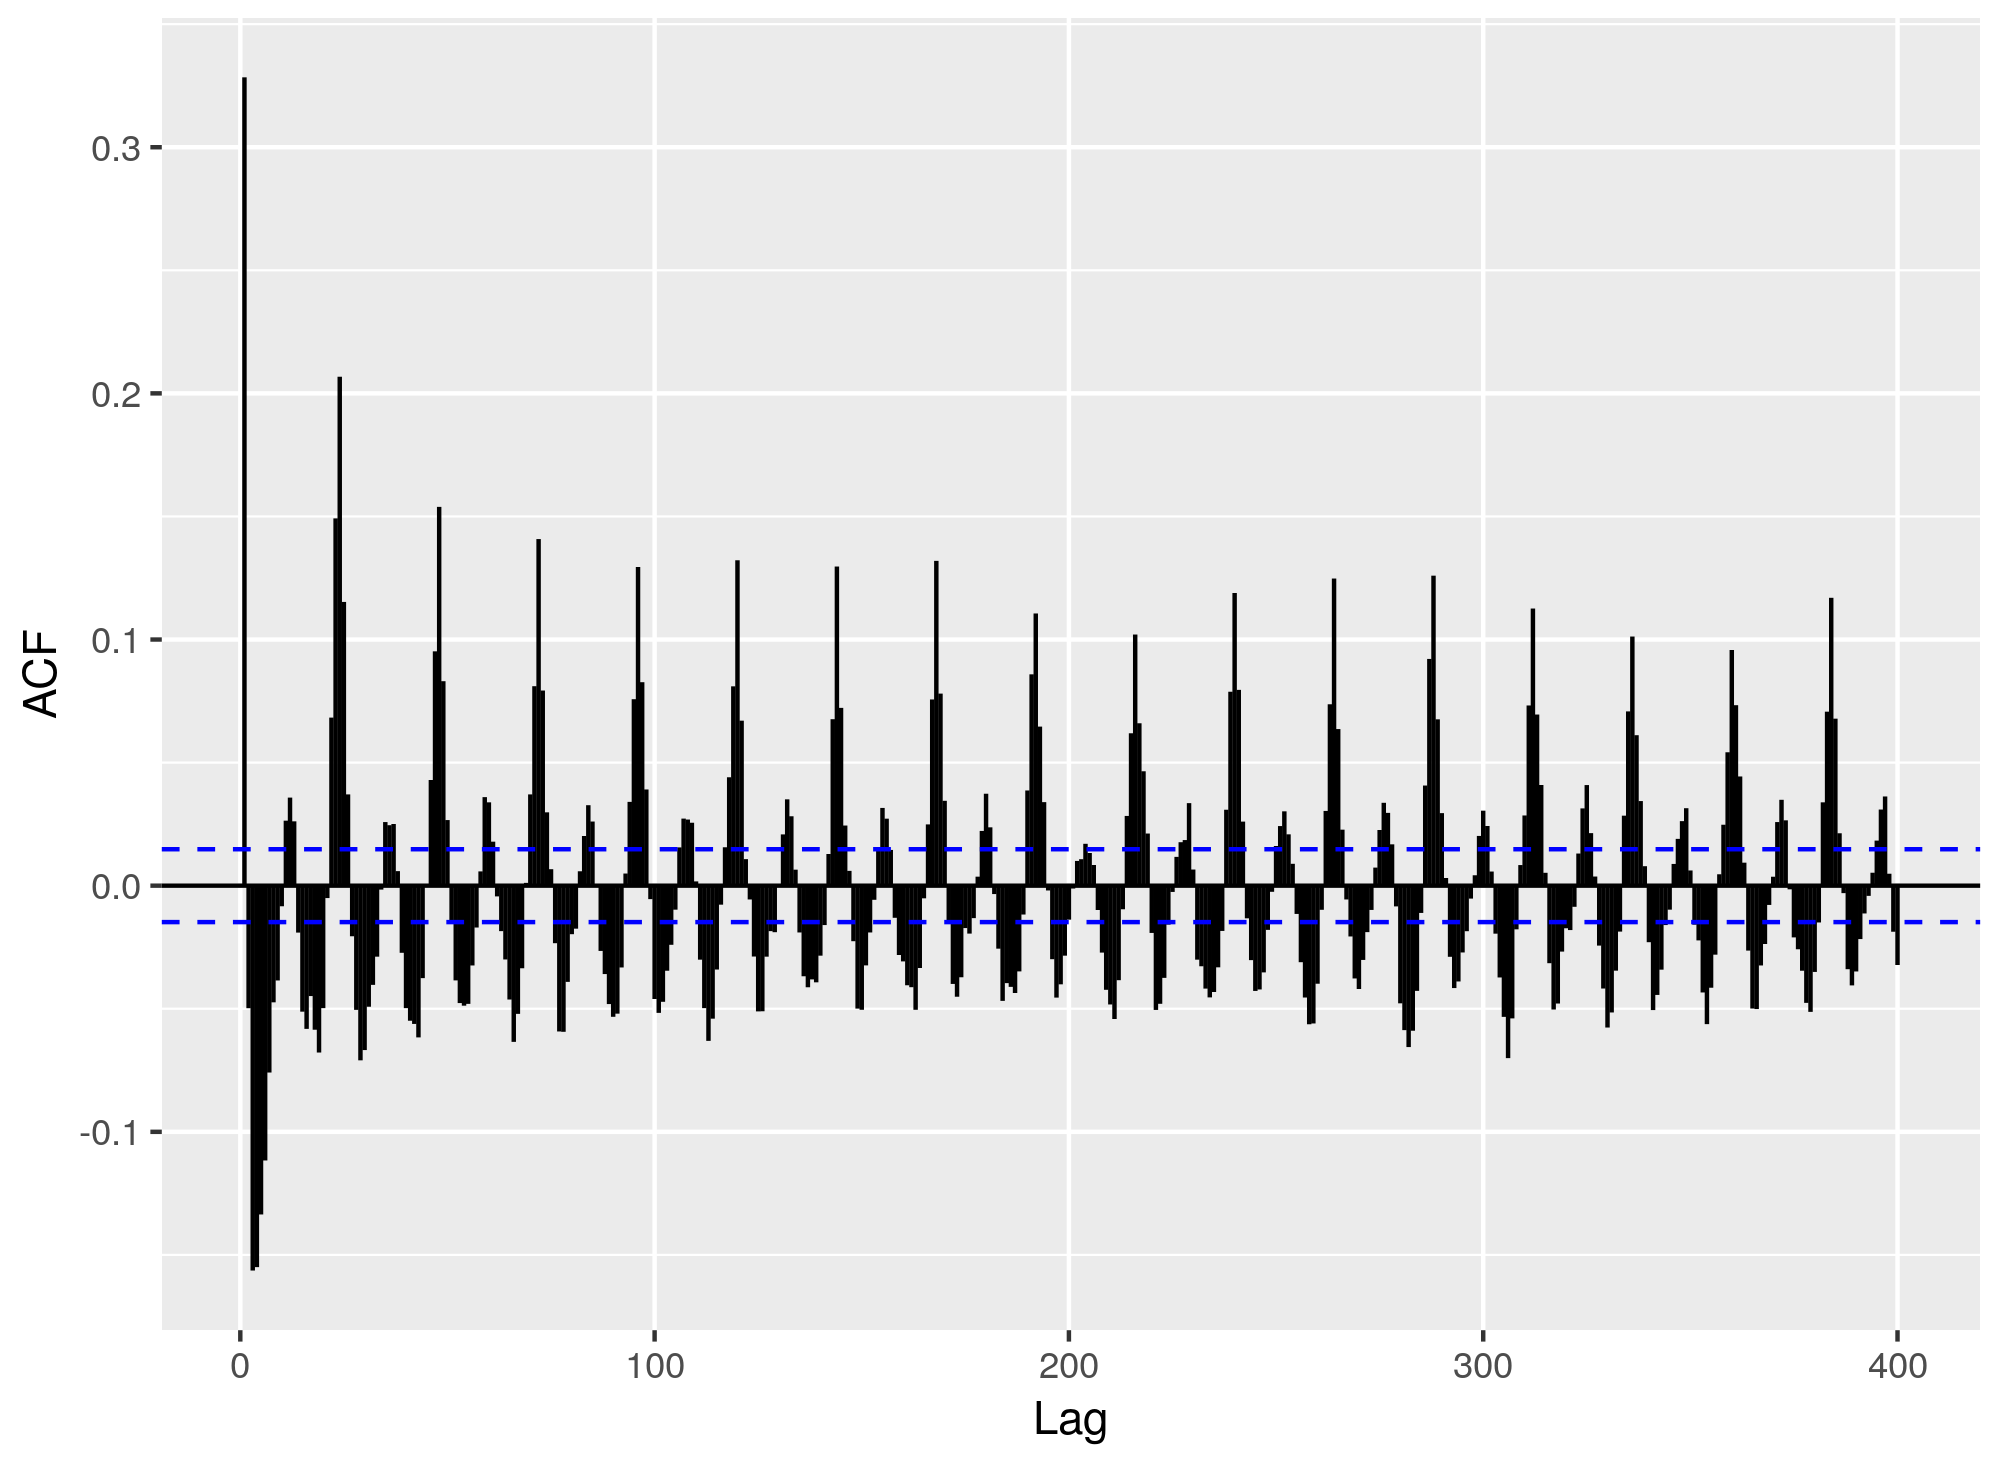
\includegraphics[scale=0.6]{long_memory_lagmax.png}
%%		\caption{Gráficos da Função de Autocorrelação (ACF) e Função de Autocorrelação Parcial (PACF)}
	\end{figure}
\end{frame}

\begin{frame}
	\frametitle{Memória Longa de Curto-Prazo}

	\begin{itemize}
		\item Modelo utilizando redes neurais
		\item Resultado insatisfatório	
		\item Longo tempo de treinamento
	\end{itemize}
	
	\begin{figure}
		\centering
		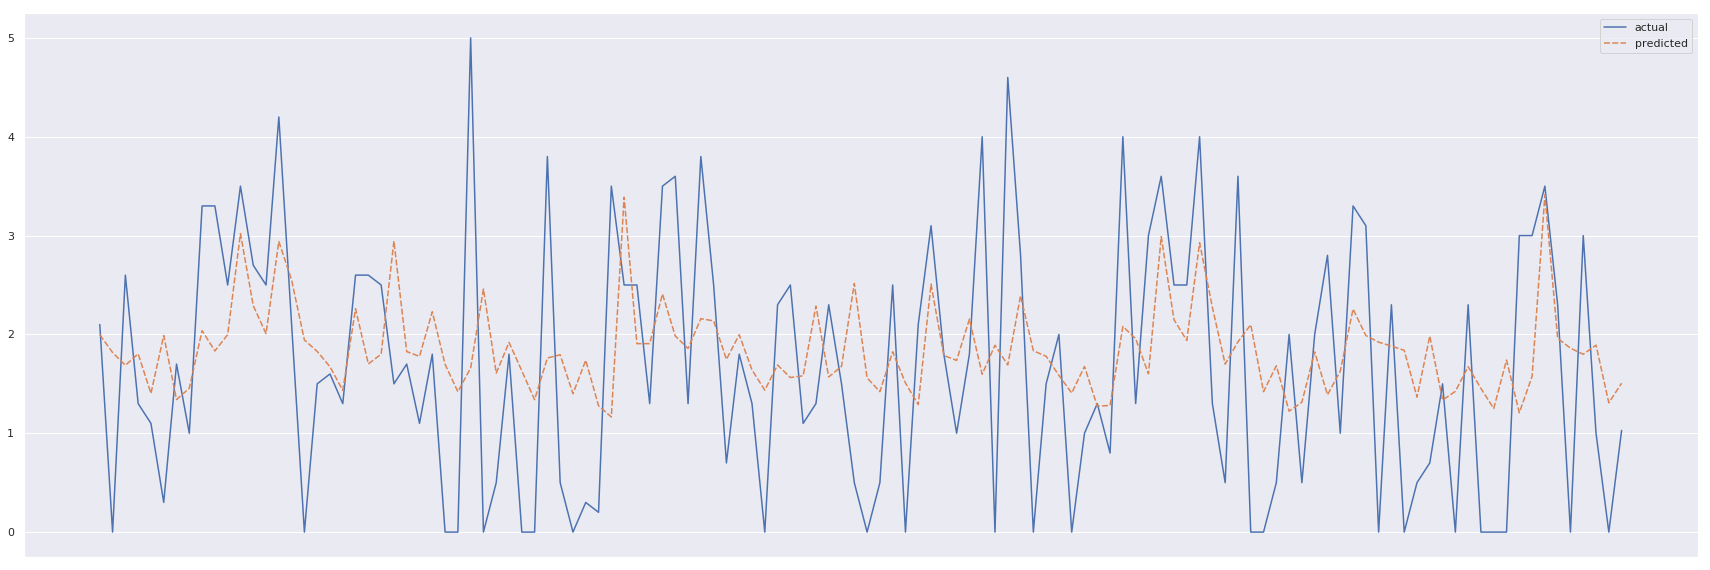
\includegraphics[width=\textwidth]{lstm.png}
		\caption{Curva em azul: dados medidos. Curva em laranja: dados previstos pelo modelo}
	\end{figure}
\end{frame}

\begin{frame}
	\frametitle{Mudança de abordagem: janela de dados (diferenciação)}
	\begin{figure}
		\centering
		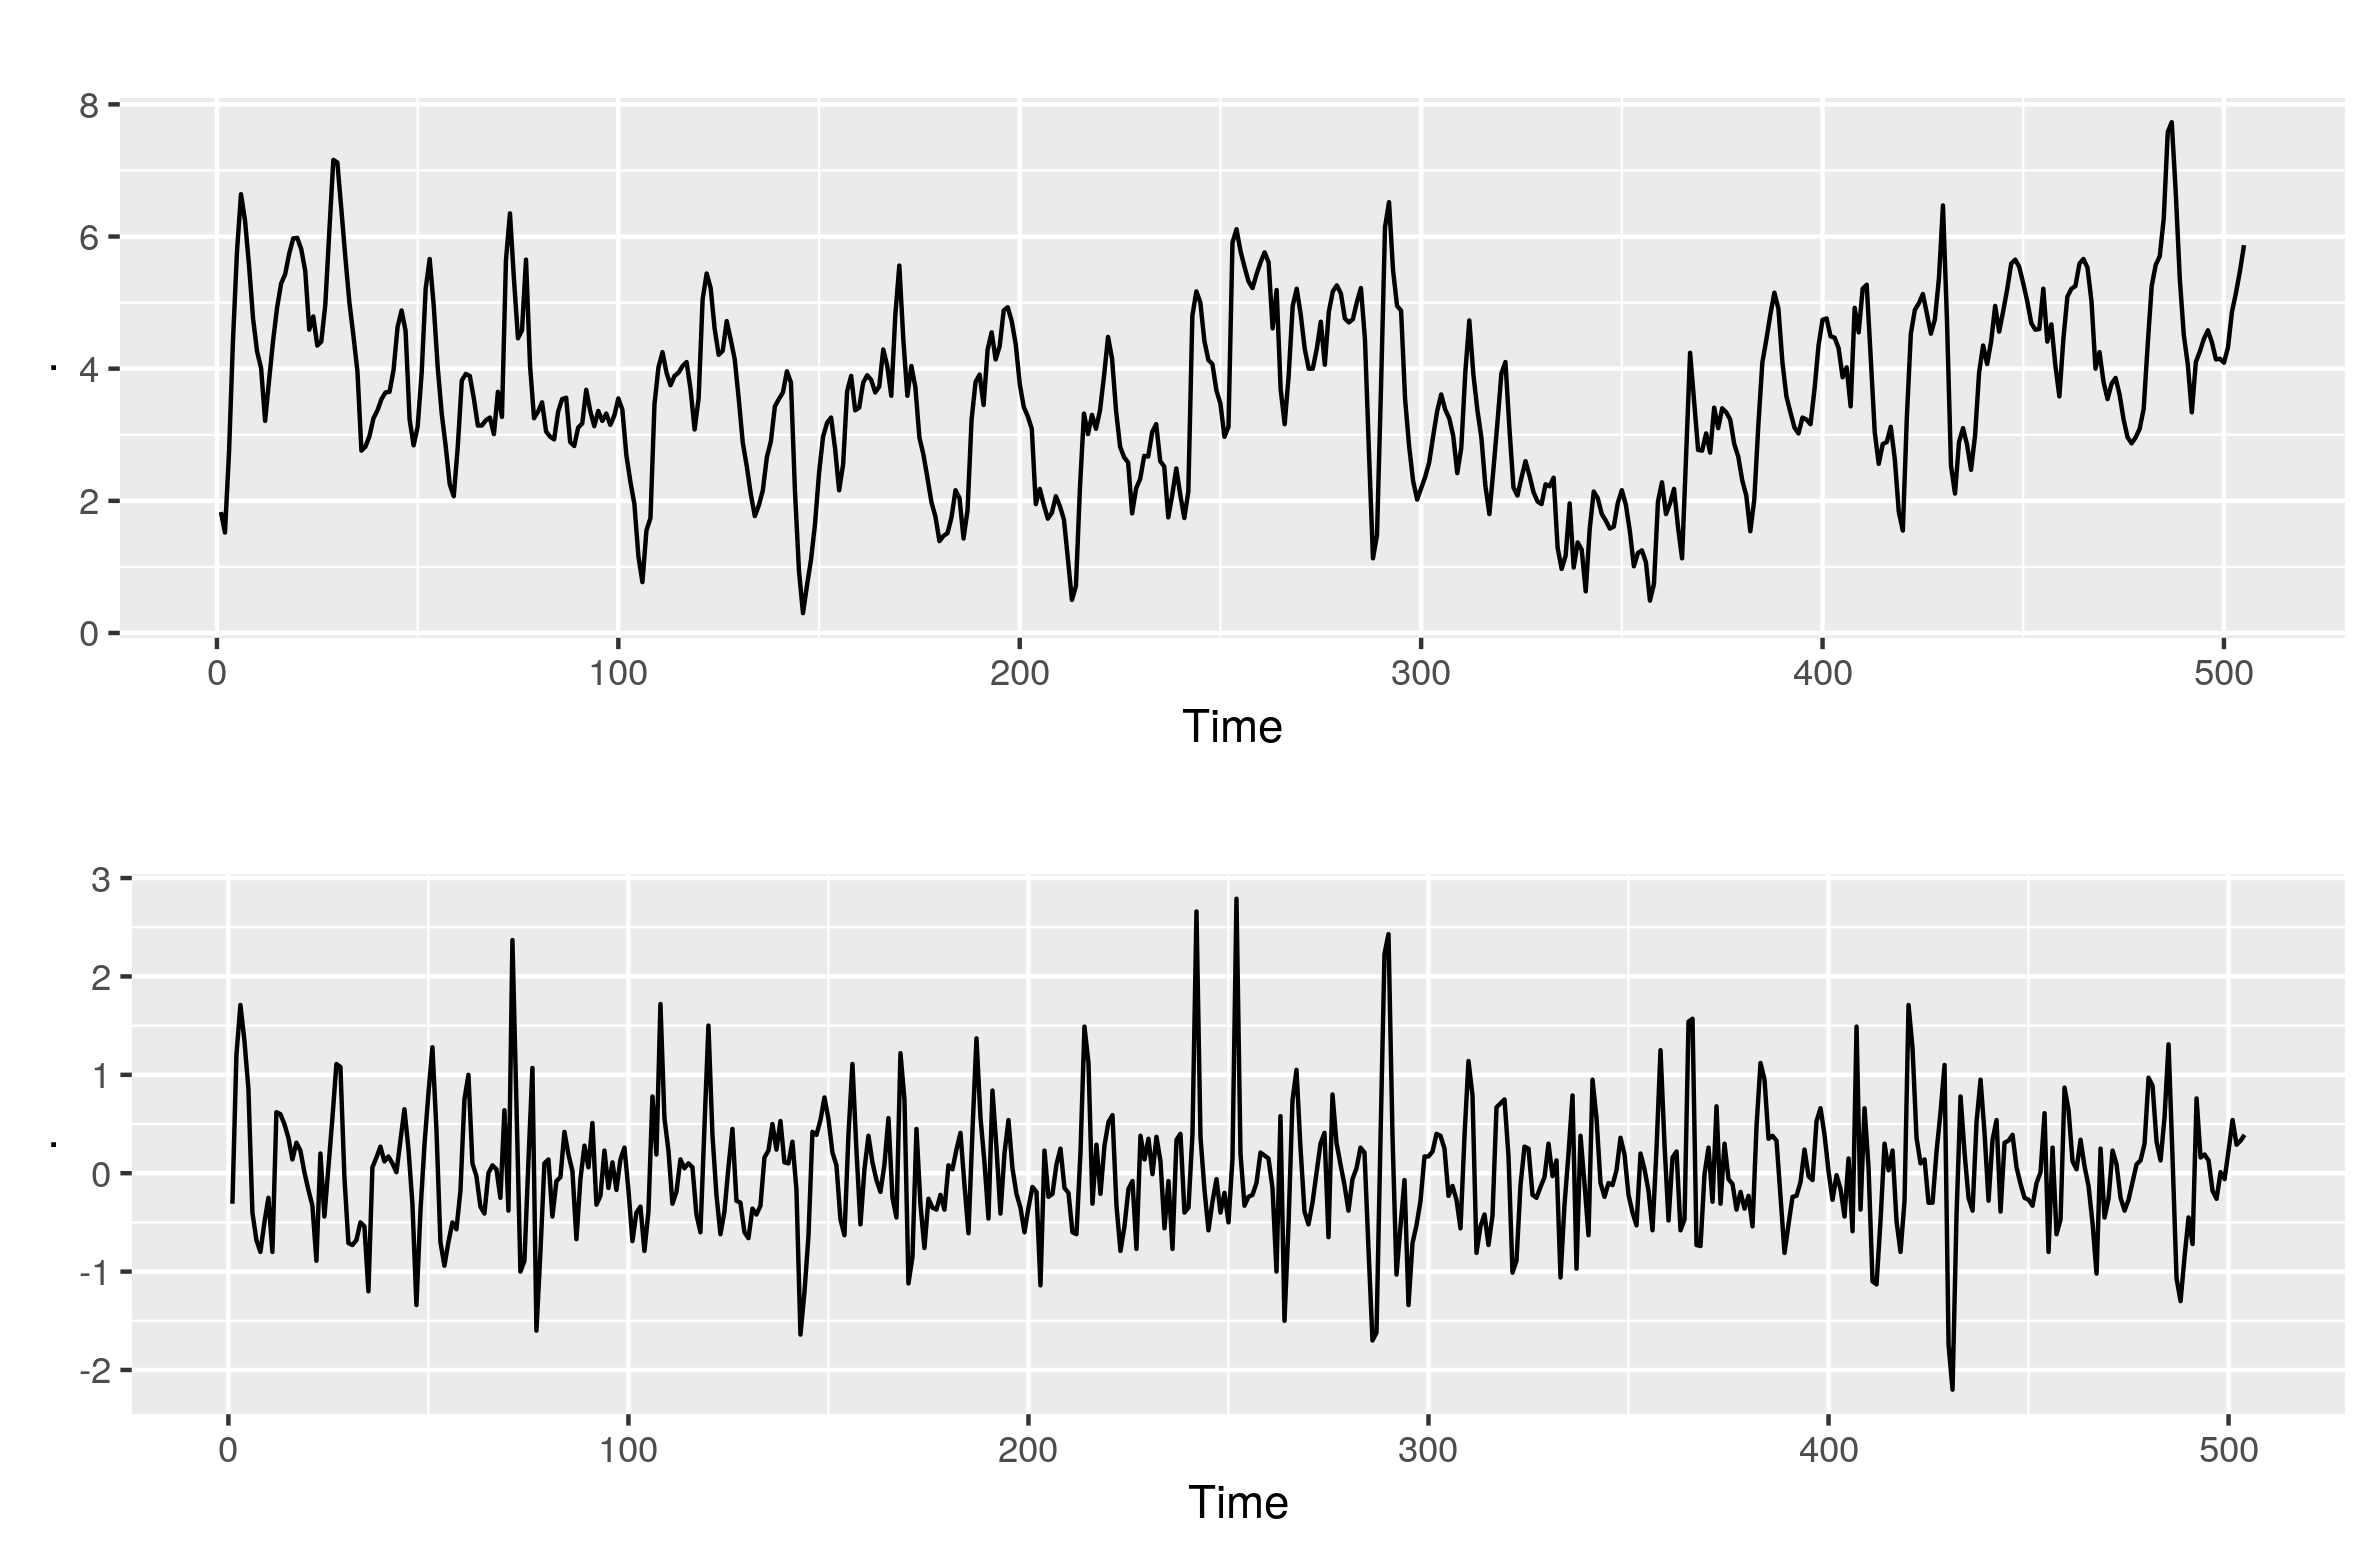
\includegraphics[scale=0.37]{last3weeks.png}
%%		\caption{3 útimas semanas de dados da série. Antes da diferenciação (superior) e após (inferior).}
	\end{figure}
\end{frame}

\begin{frame}
	\frametitle{Novas funções de autocorrelação}
	\begin{figure}
		\centering
		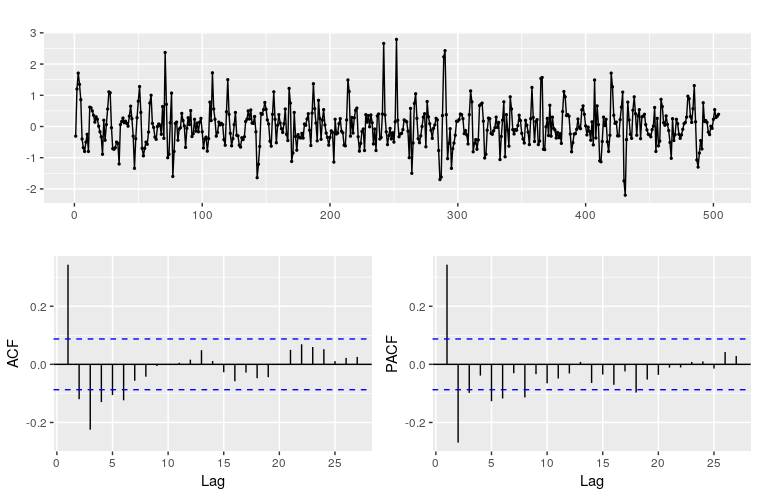
\includegraphics[scale=0.4]{last3weeks_acf.png}
%%		\caption{Gráficos da Função de Autocorrelação e Autocorrelação Parical para 2 semanas de dados da série.}
	\end{figure}
\end{frame}

\begin{frame}	
	\frametitle{Mensurando o erro de previsão: $e_{t+h} = y_{t+h} - \hat{y}_{t+h}$}

	\begin{block}{Erro médio absoluto (MAE)}
		\begin{equation*}
			\text{MAE} = \frac{1}{T}\sum_{t=1}^{T}\left|e_{t}\right|
		\end{equation*}
	\end{block}
	
	\pause

	\begin{block}{Raíz do quadrado da média do erro (RMSE)}
		\begin{equation*}
			\text{RMSE} = \sqrt{\frac{1}{T}\sum_{t=1}^{T}e_{t}^2}
		\end{equation*}
	\end{block}

	\pause

	\begin{block}{Erro absoluto médio escalonado (MASE)}
		\begin{equation*}
			\text{MASE} = \frac{\frac{1}{T}\sum_{t=1}^T\left|e_t\right|}{\frac{1}{T-1}\sum_{t=2}^{T}\left|y_t-y_{t-1}\right|}
		\end{equation*}
	\end{block}
\end{frame}

\begin{frame}
	\frametitle{Validação cruzada: conjunto de treinamento e de teste}
	\begin{figure}
		\centering
		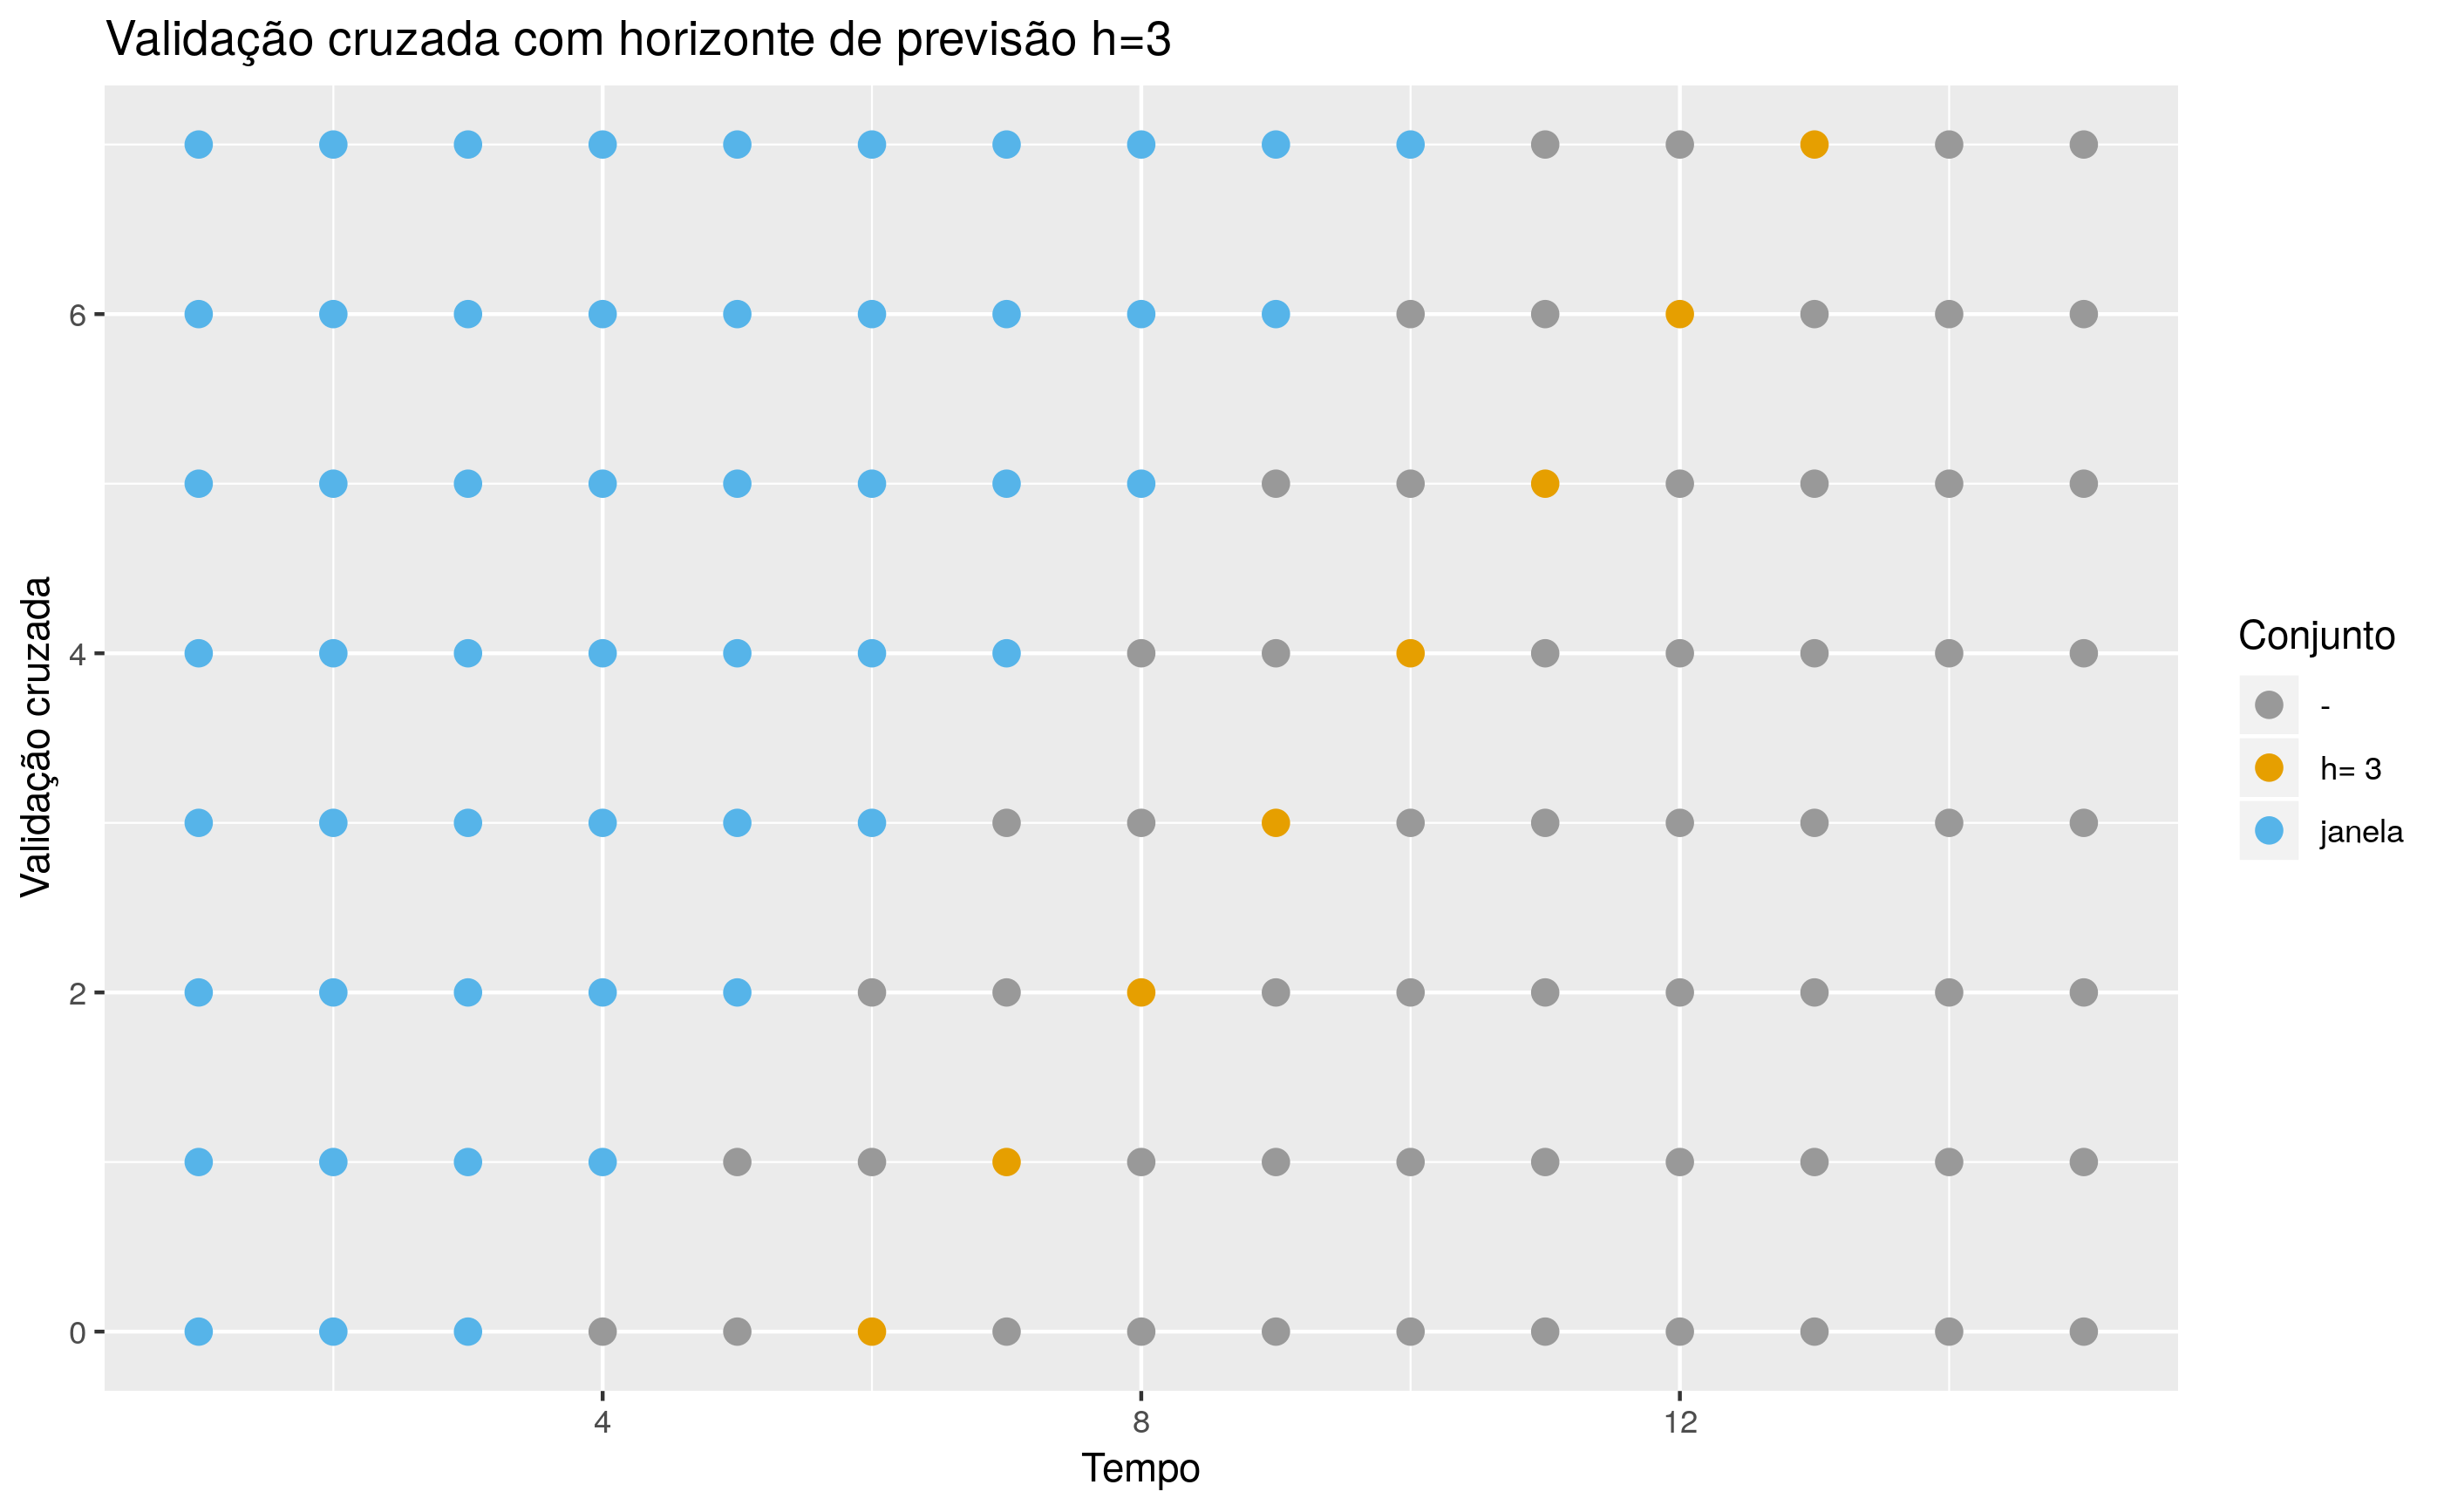
\includegraphics[scale=0.5]{crossh3}
%%		\caption{Chapada}
	\end{figure}
\end{frame}

\begin{frame}
	\frametitle{Estabilidade: regime estacionário e inversibilidade}
	\begin{figure}
		\centering
		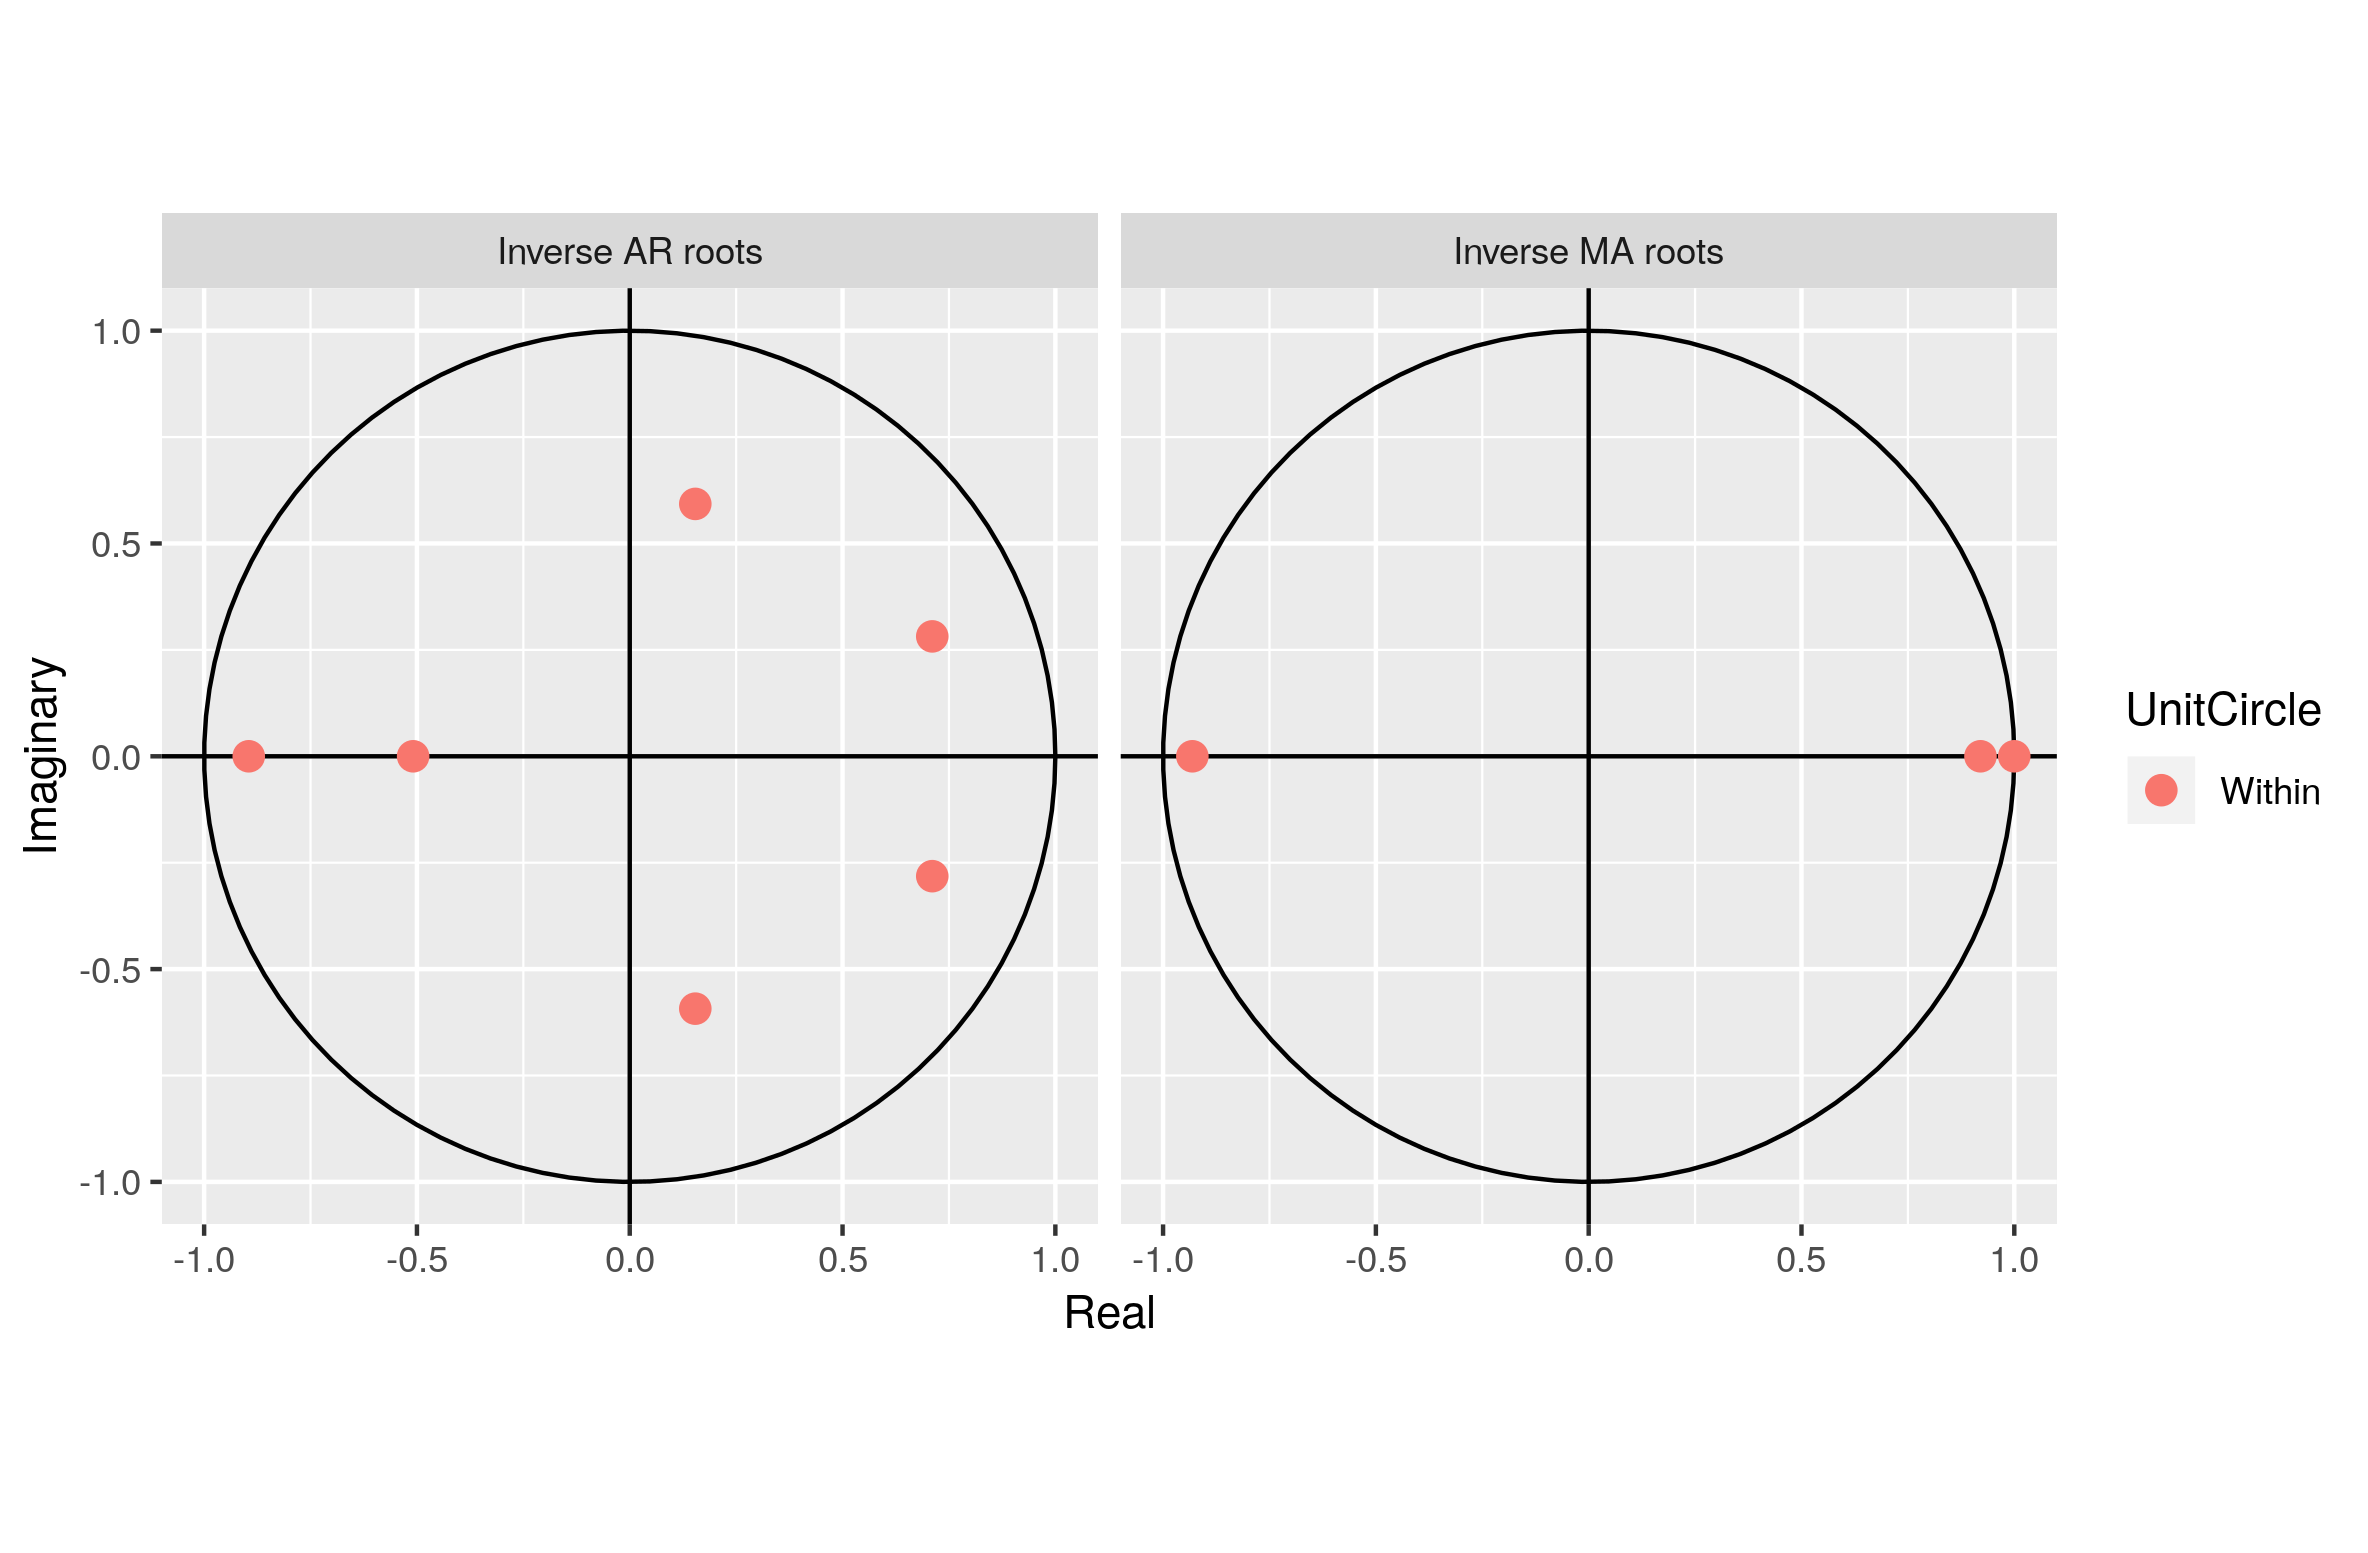
\includegraphics[width=\textwidth]{conds}
%%		\caption{Condições de regime estacionário e invertibilidade para um modelo ARIMA(6,1,0).}
	\end{figure}
\end{frame}

\begin{frame}
	\frametitle{Previsões com modelo ARIMA}
	\begin{figure}
		\centering
		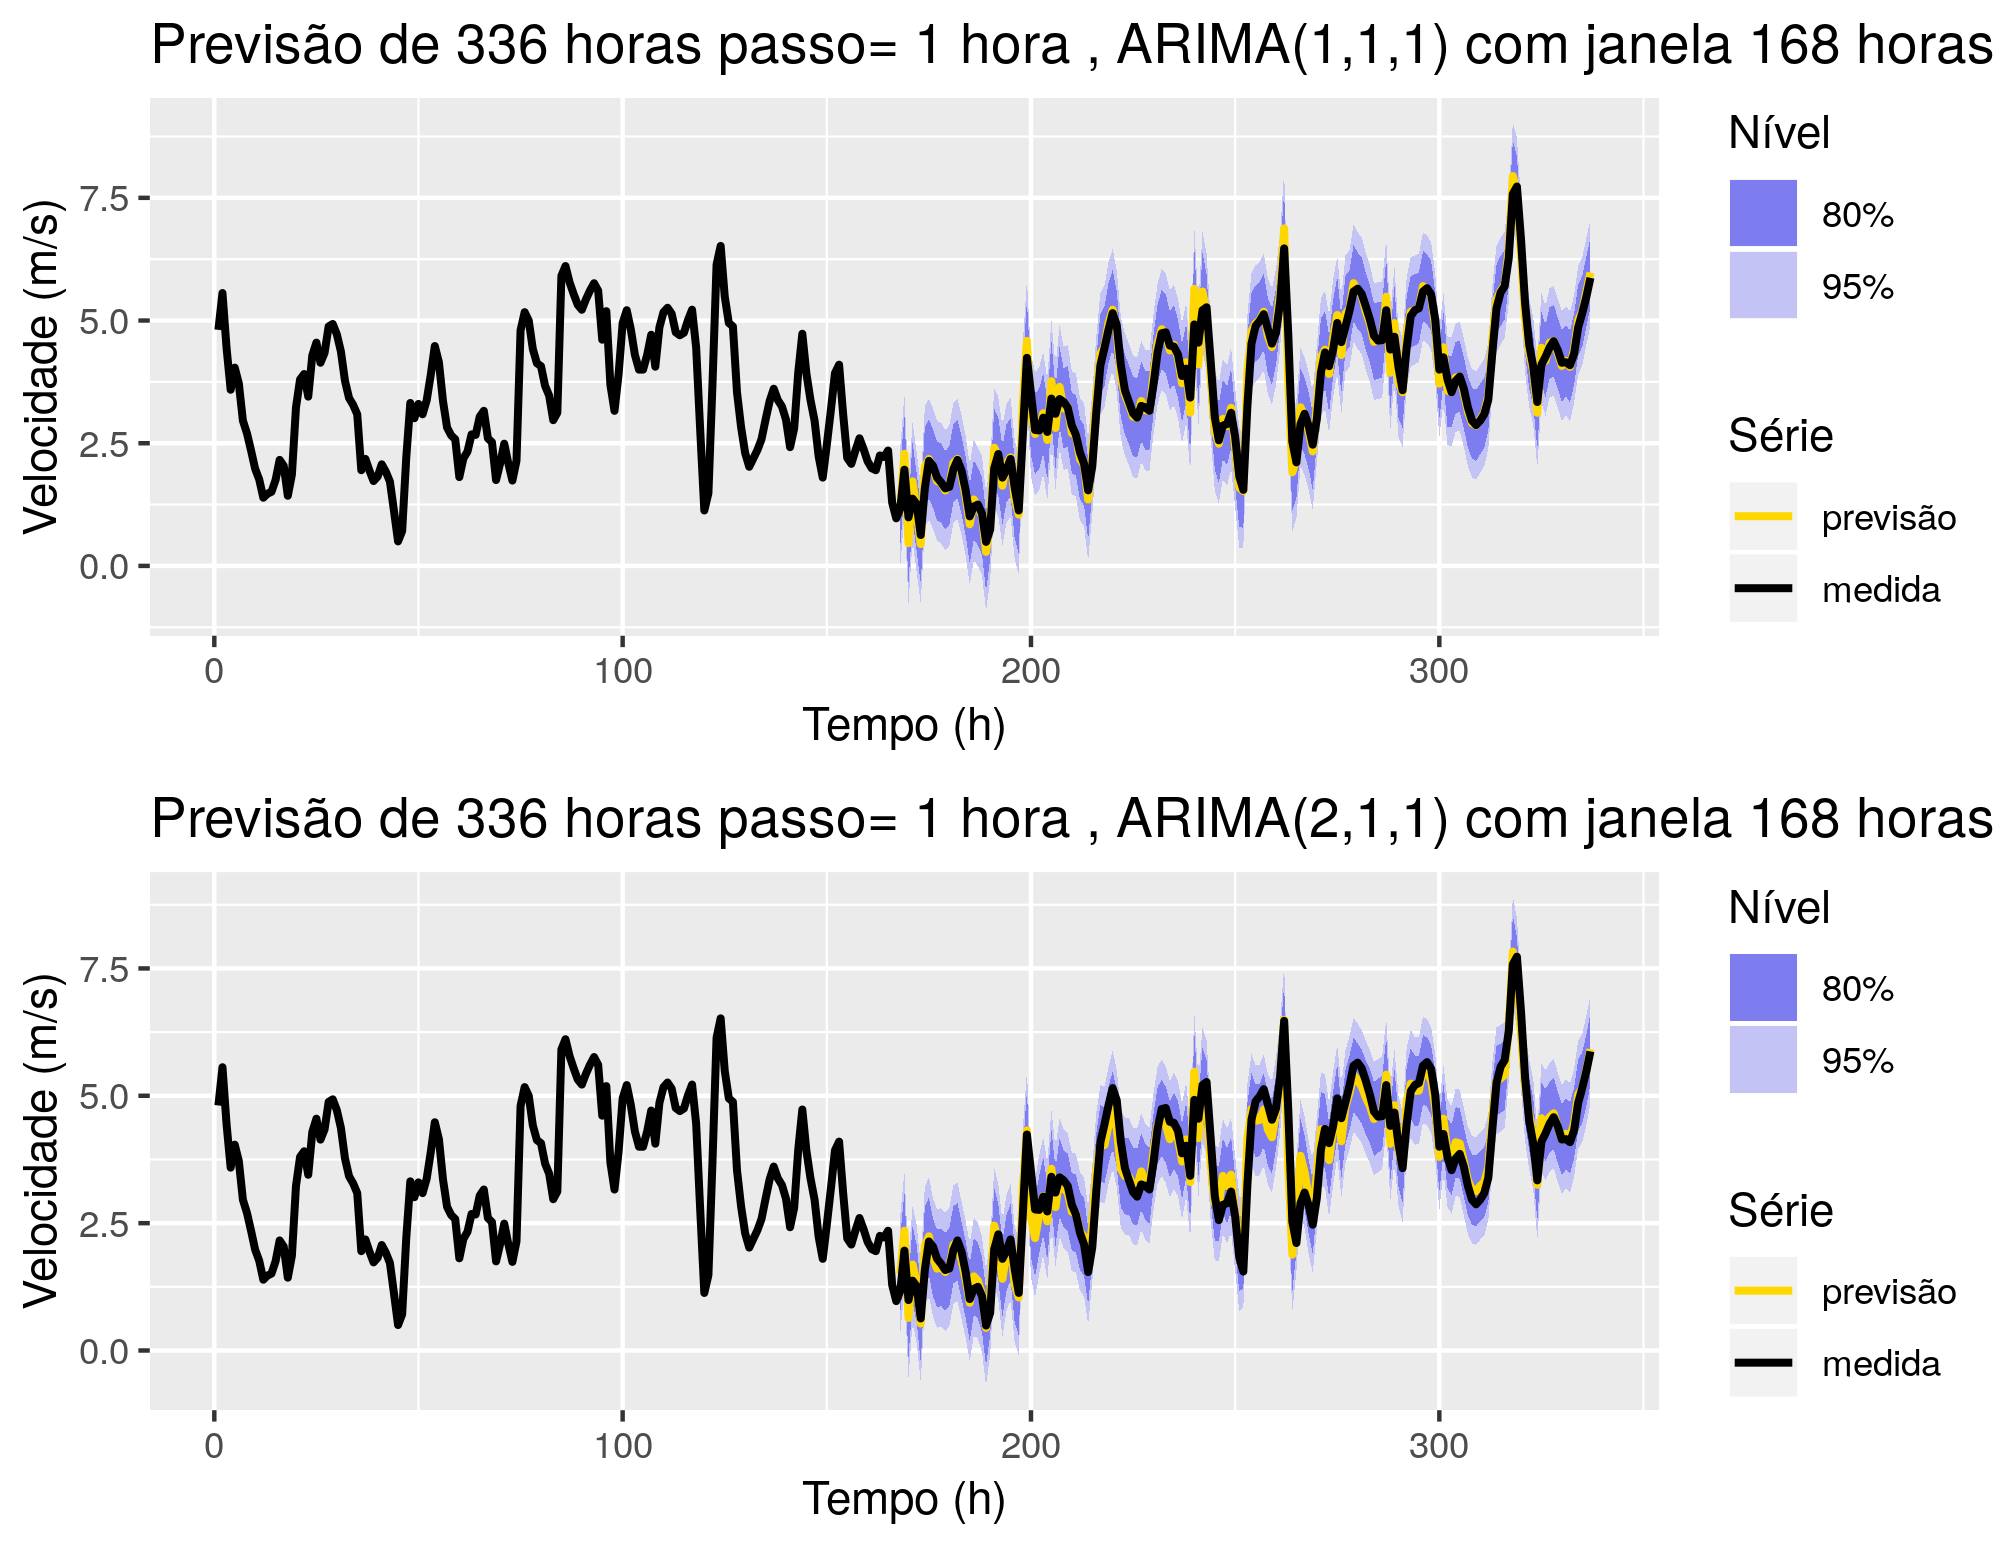
\includegraphics[scale=0.6]{arima12}
%%		\caption{Condições de regime estacionário e invertibilidade para um modelo ARIMA(6,1,0).}
	\end{figure}
\end{frame}

\begin{frame}
	\frametitle{Previsões com modelo ARIMA}
	\begin{figure}
		\centering
		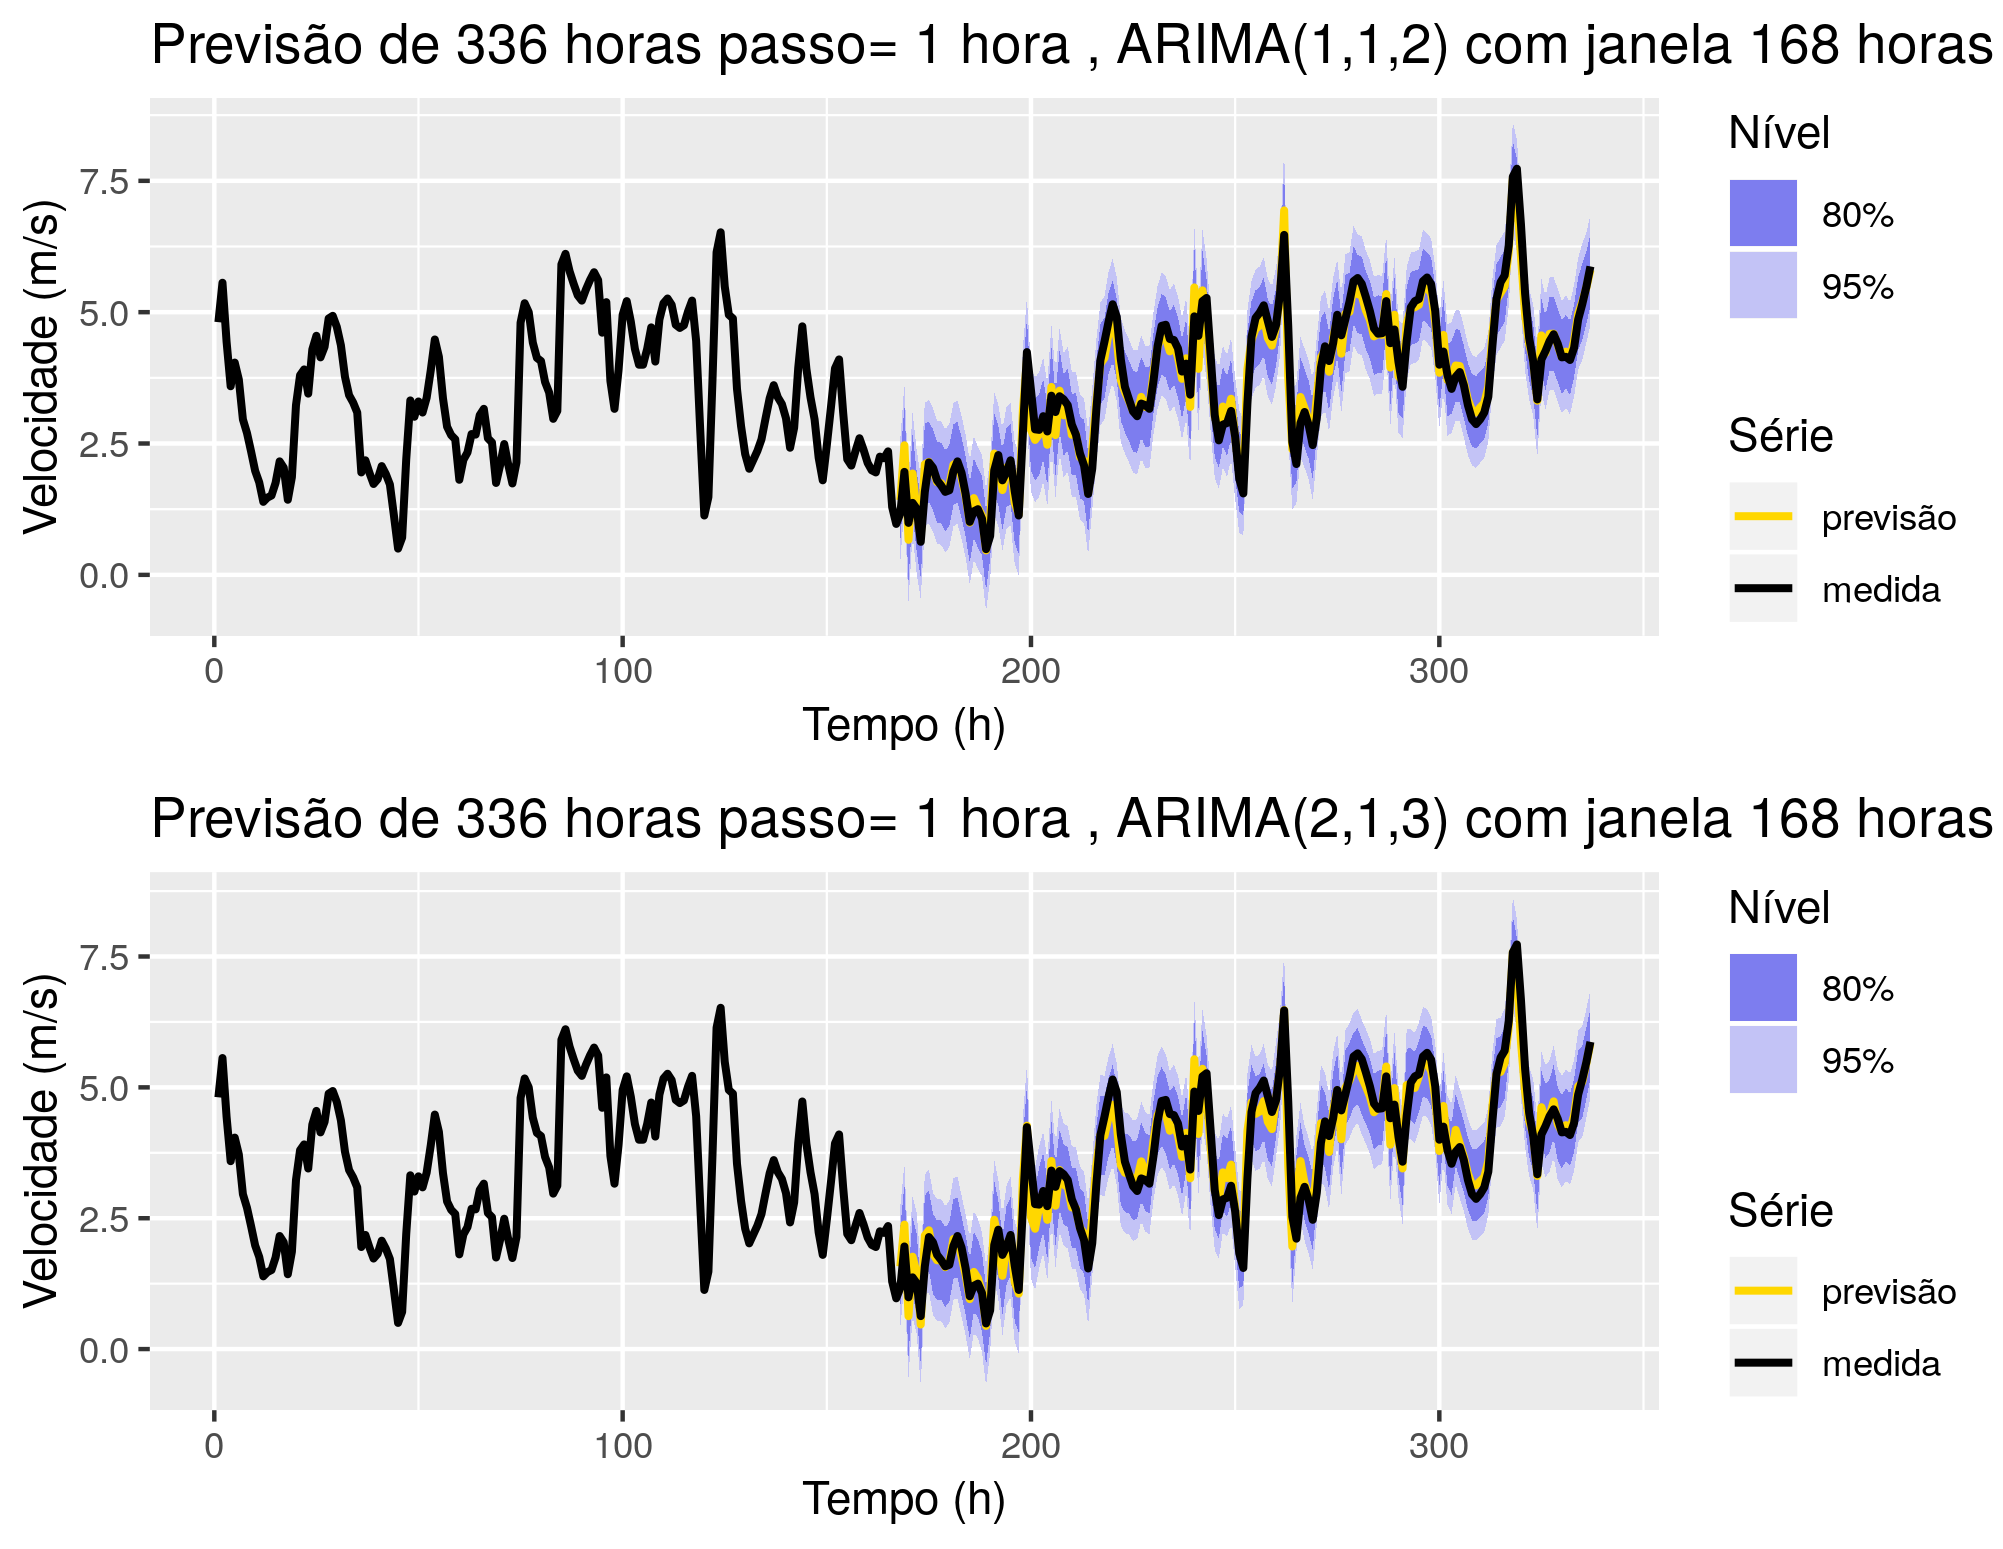
\includegraphics[scale=0.6]{arima34}
%%		\caption{Condições de regime estacionário e invertibilidade para um modelo ARIMA(6,1,0).}
	\end{figure}
\end{frame}

\begin{frame}
	\frametitle{Medidas de erro}
	\begin{table}[h]
		\centering
		\begin{tabular}{ |c|c|c|c|c|c| } 
			\hline
			\textbf{ARIMA(p,d,q)}&\textbf{ME}&\textbf{RMSE}&\textbf{MAE}&\textbf{MPE}&\textbf{MASE}\\
			\hline
			1,1,1&-0.008&0.223&0.162&0.382&5.731 \\
			\hline
			2,1,1&0.008&0.297&0.228&-0.756&7.622 \\
			\hline
			1,1,2&0.016&0.249&0.187&-0.839&6.152 \\
			\hline
			2,1,3&0.0158&0.319&0.238&-0.838&7.968 \\
			\hline
		\end{tabular}
		\caption{Medidas de erro para 4 modelos ARIMA aplicados à séries modelo.}
	\end{table}
\end{frame}

\subsection{Modelo Autorregressivo Variável}

\begin{frame}
	\frametitle{Modelo Autorregressivo Variável}
	\begin{itemize}
		\item<1-> Um único modelo ARIMA estático não é capaz de capturar a dinâmica da série temporal
		\item<2-> Diferentes janelas de dados apresentam diferentes parâmetros p,q ótimos		
	\end{itemize}	
\end{frame}

\begin{frame}
	\frametitle{Evolução dos parâmetros p e q de um modelo ARIMA ao longo do tempo}
	\begin{figure}
		\centering
		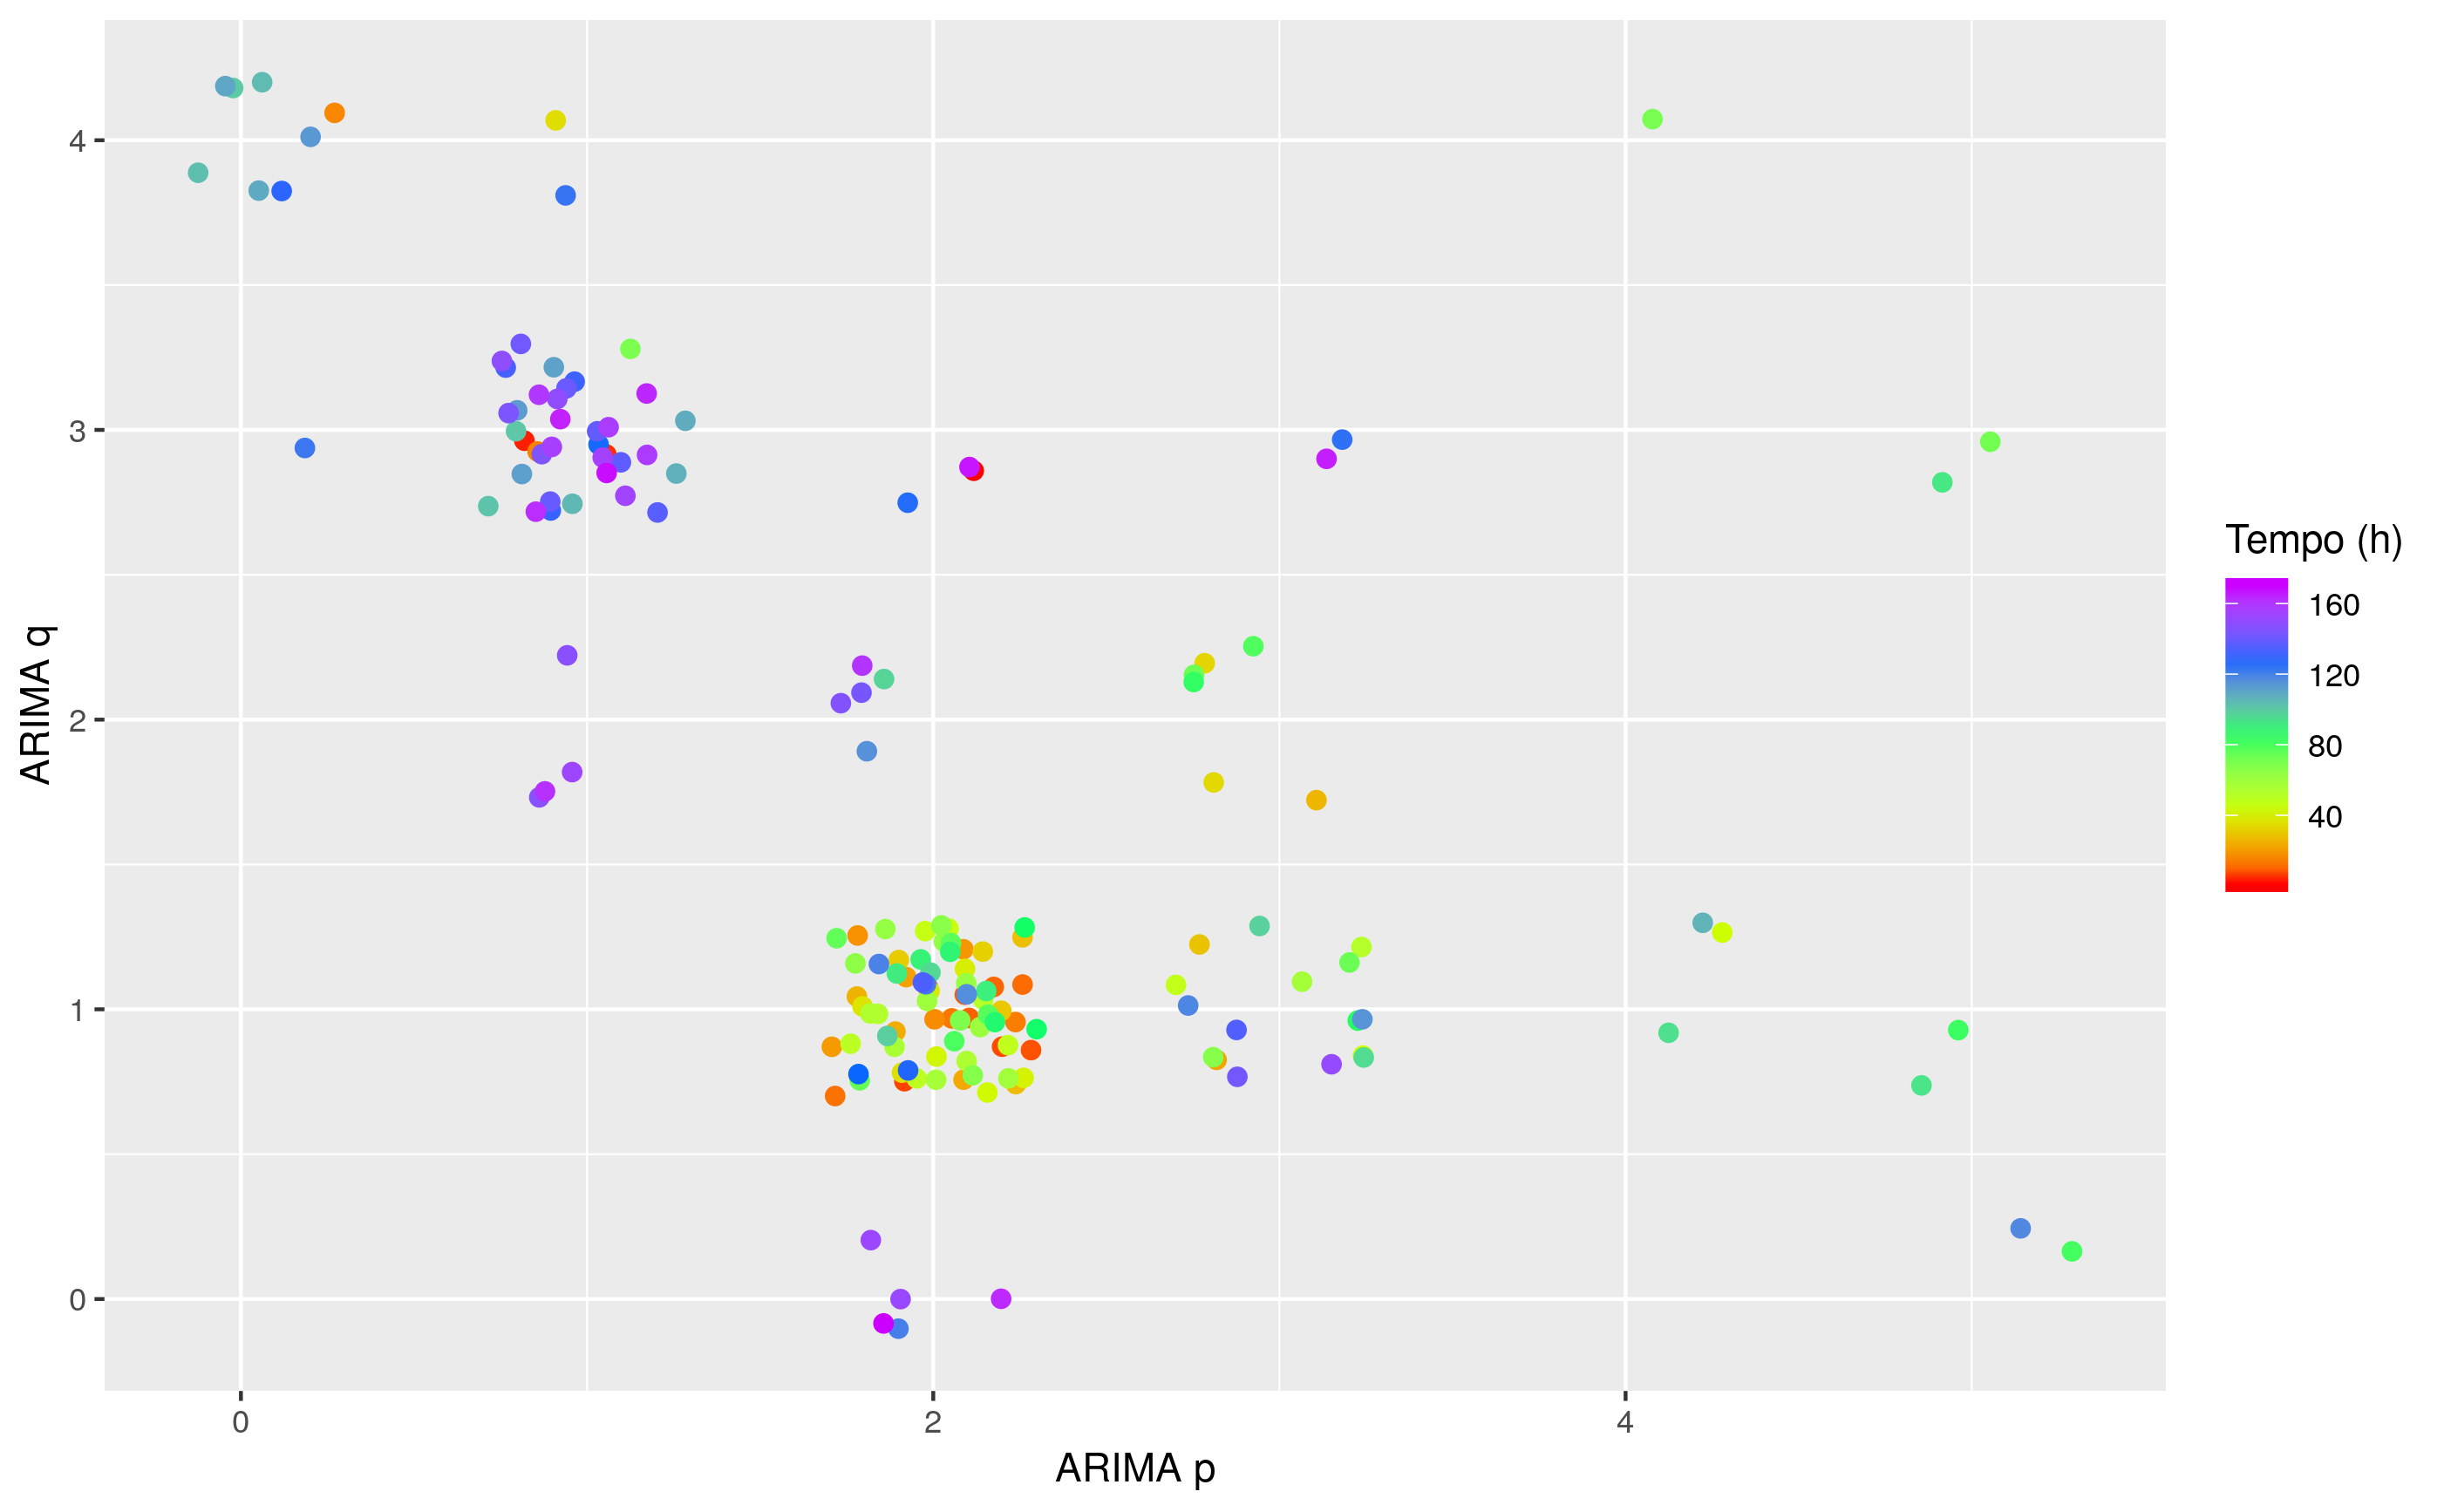
\includegraphics[scale=0.45]{var_arima}
%%		\caption{Evolução dos parâmetros p e q de um modelo ARIMA ao longo do tempo.}
	\end{figure}
\end{frame}

\begin{frame}
	\frametitle{Previsão utilizando modelo ARIMA adaptativo}
	\begin{figure}
		\centering
		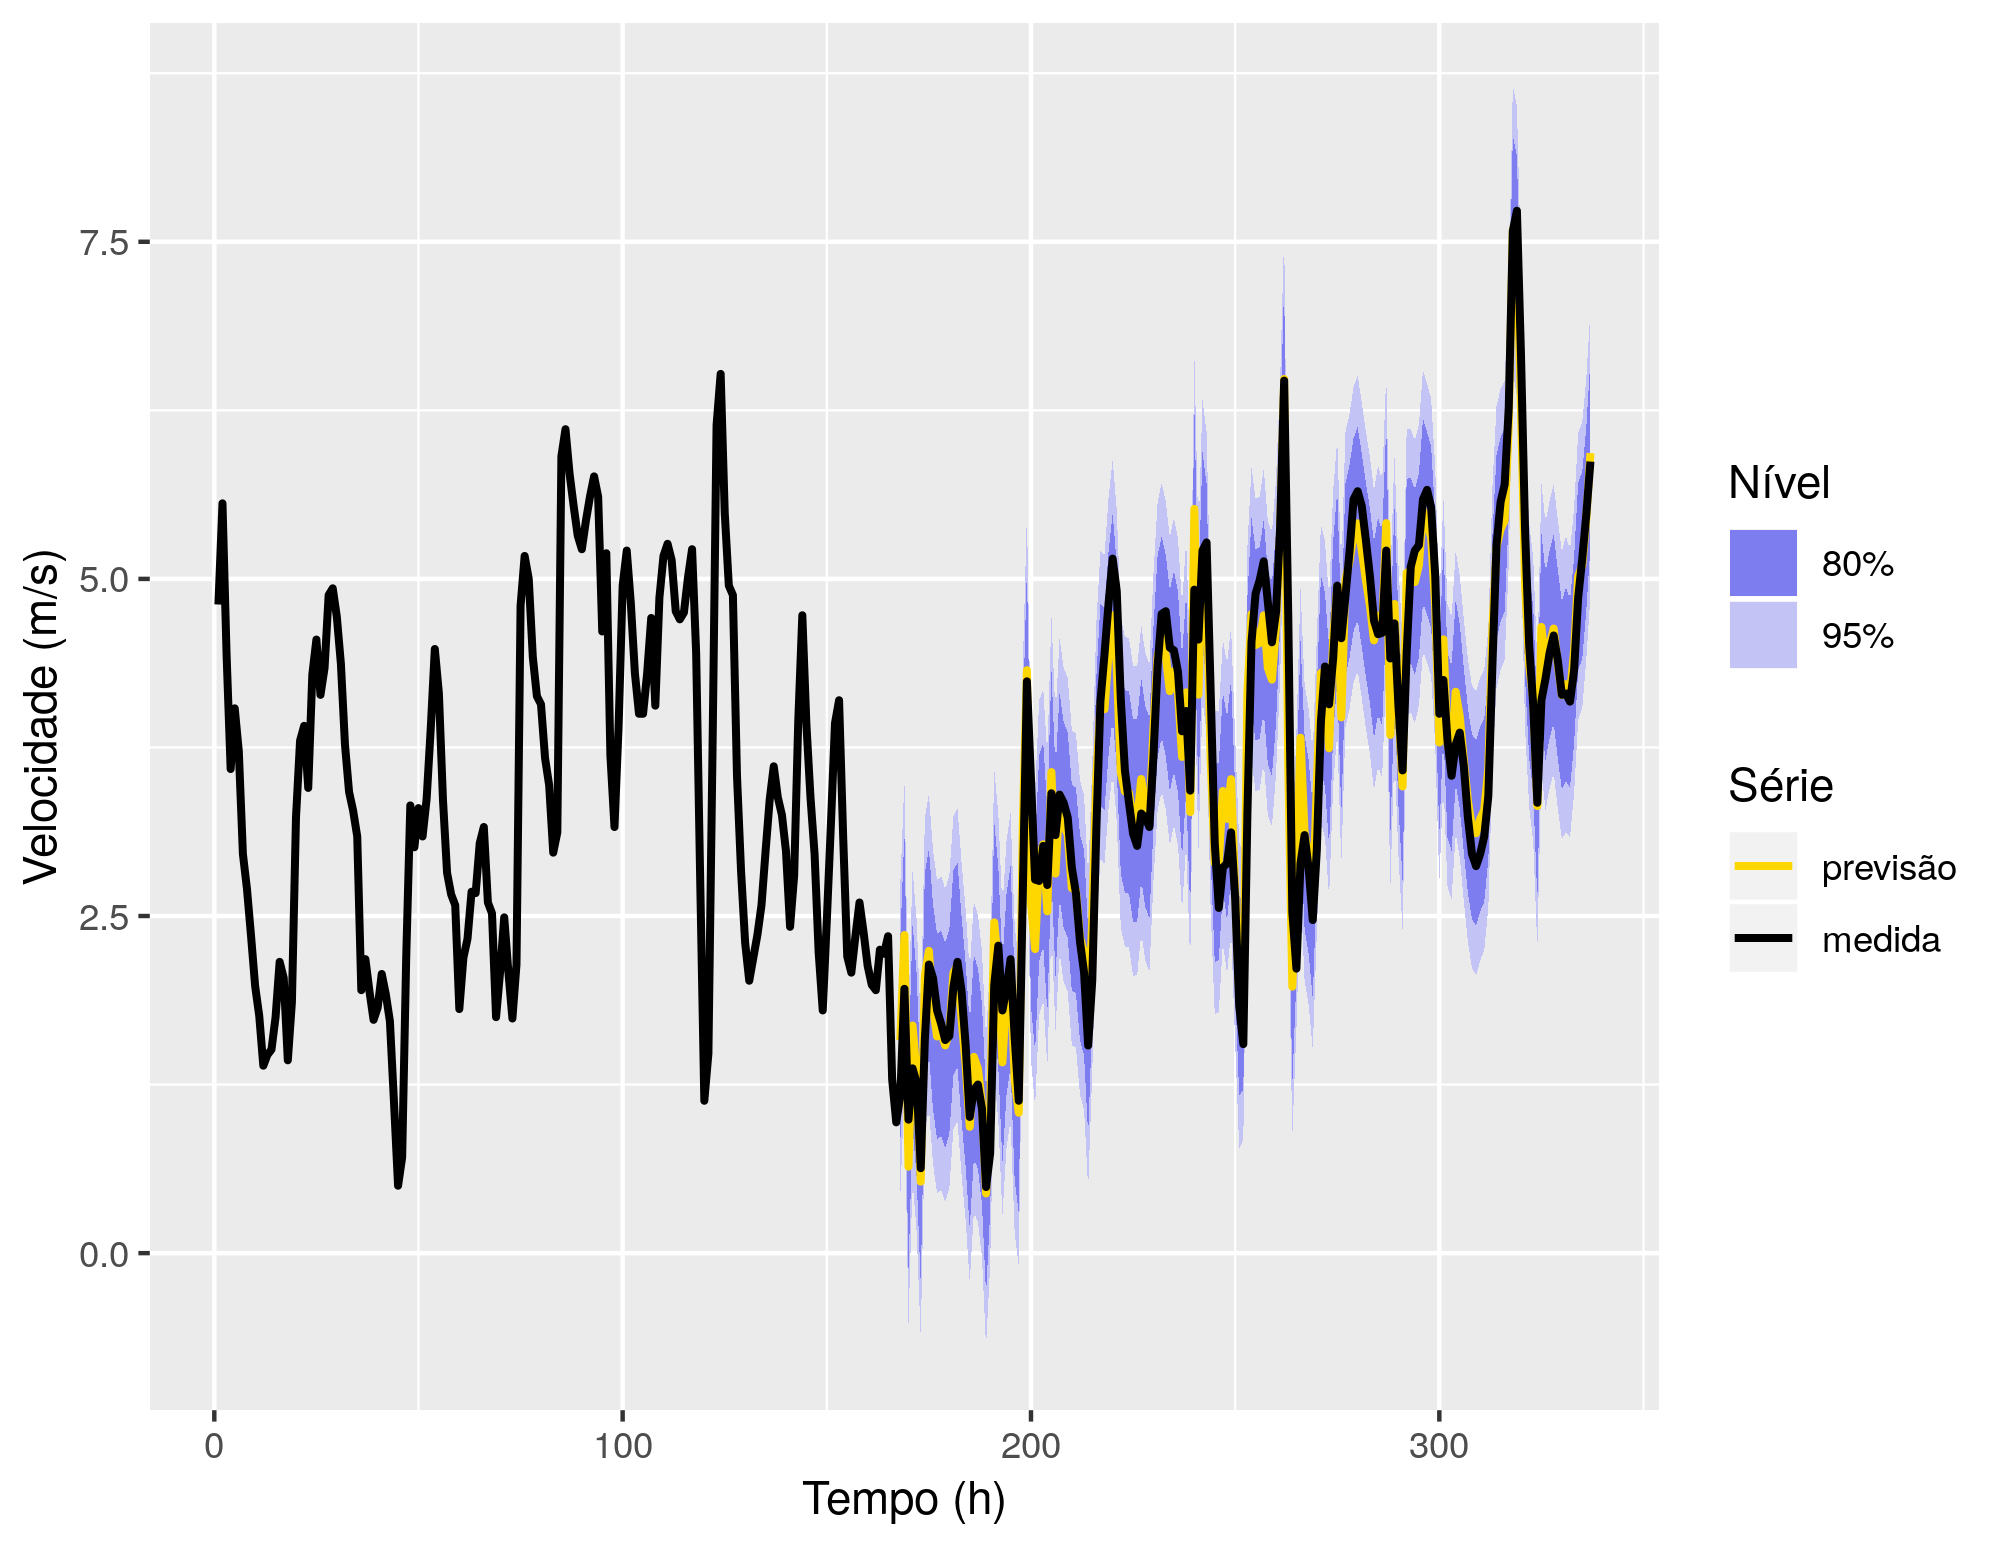
\includegraphics[scale=0.6]{var_result}
%%		\caption{Evolução dos parâmetros p e q de um modelo ARIMA ao longo do tempo.}
	\end{figure}
\end{frame}

\subsection{GARCH}

\begin{frame}
	\frametitle{Incorporando a variância}
	\begin{figure}
		\centering
		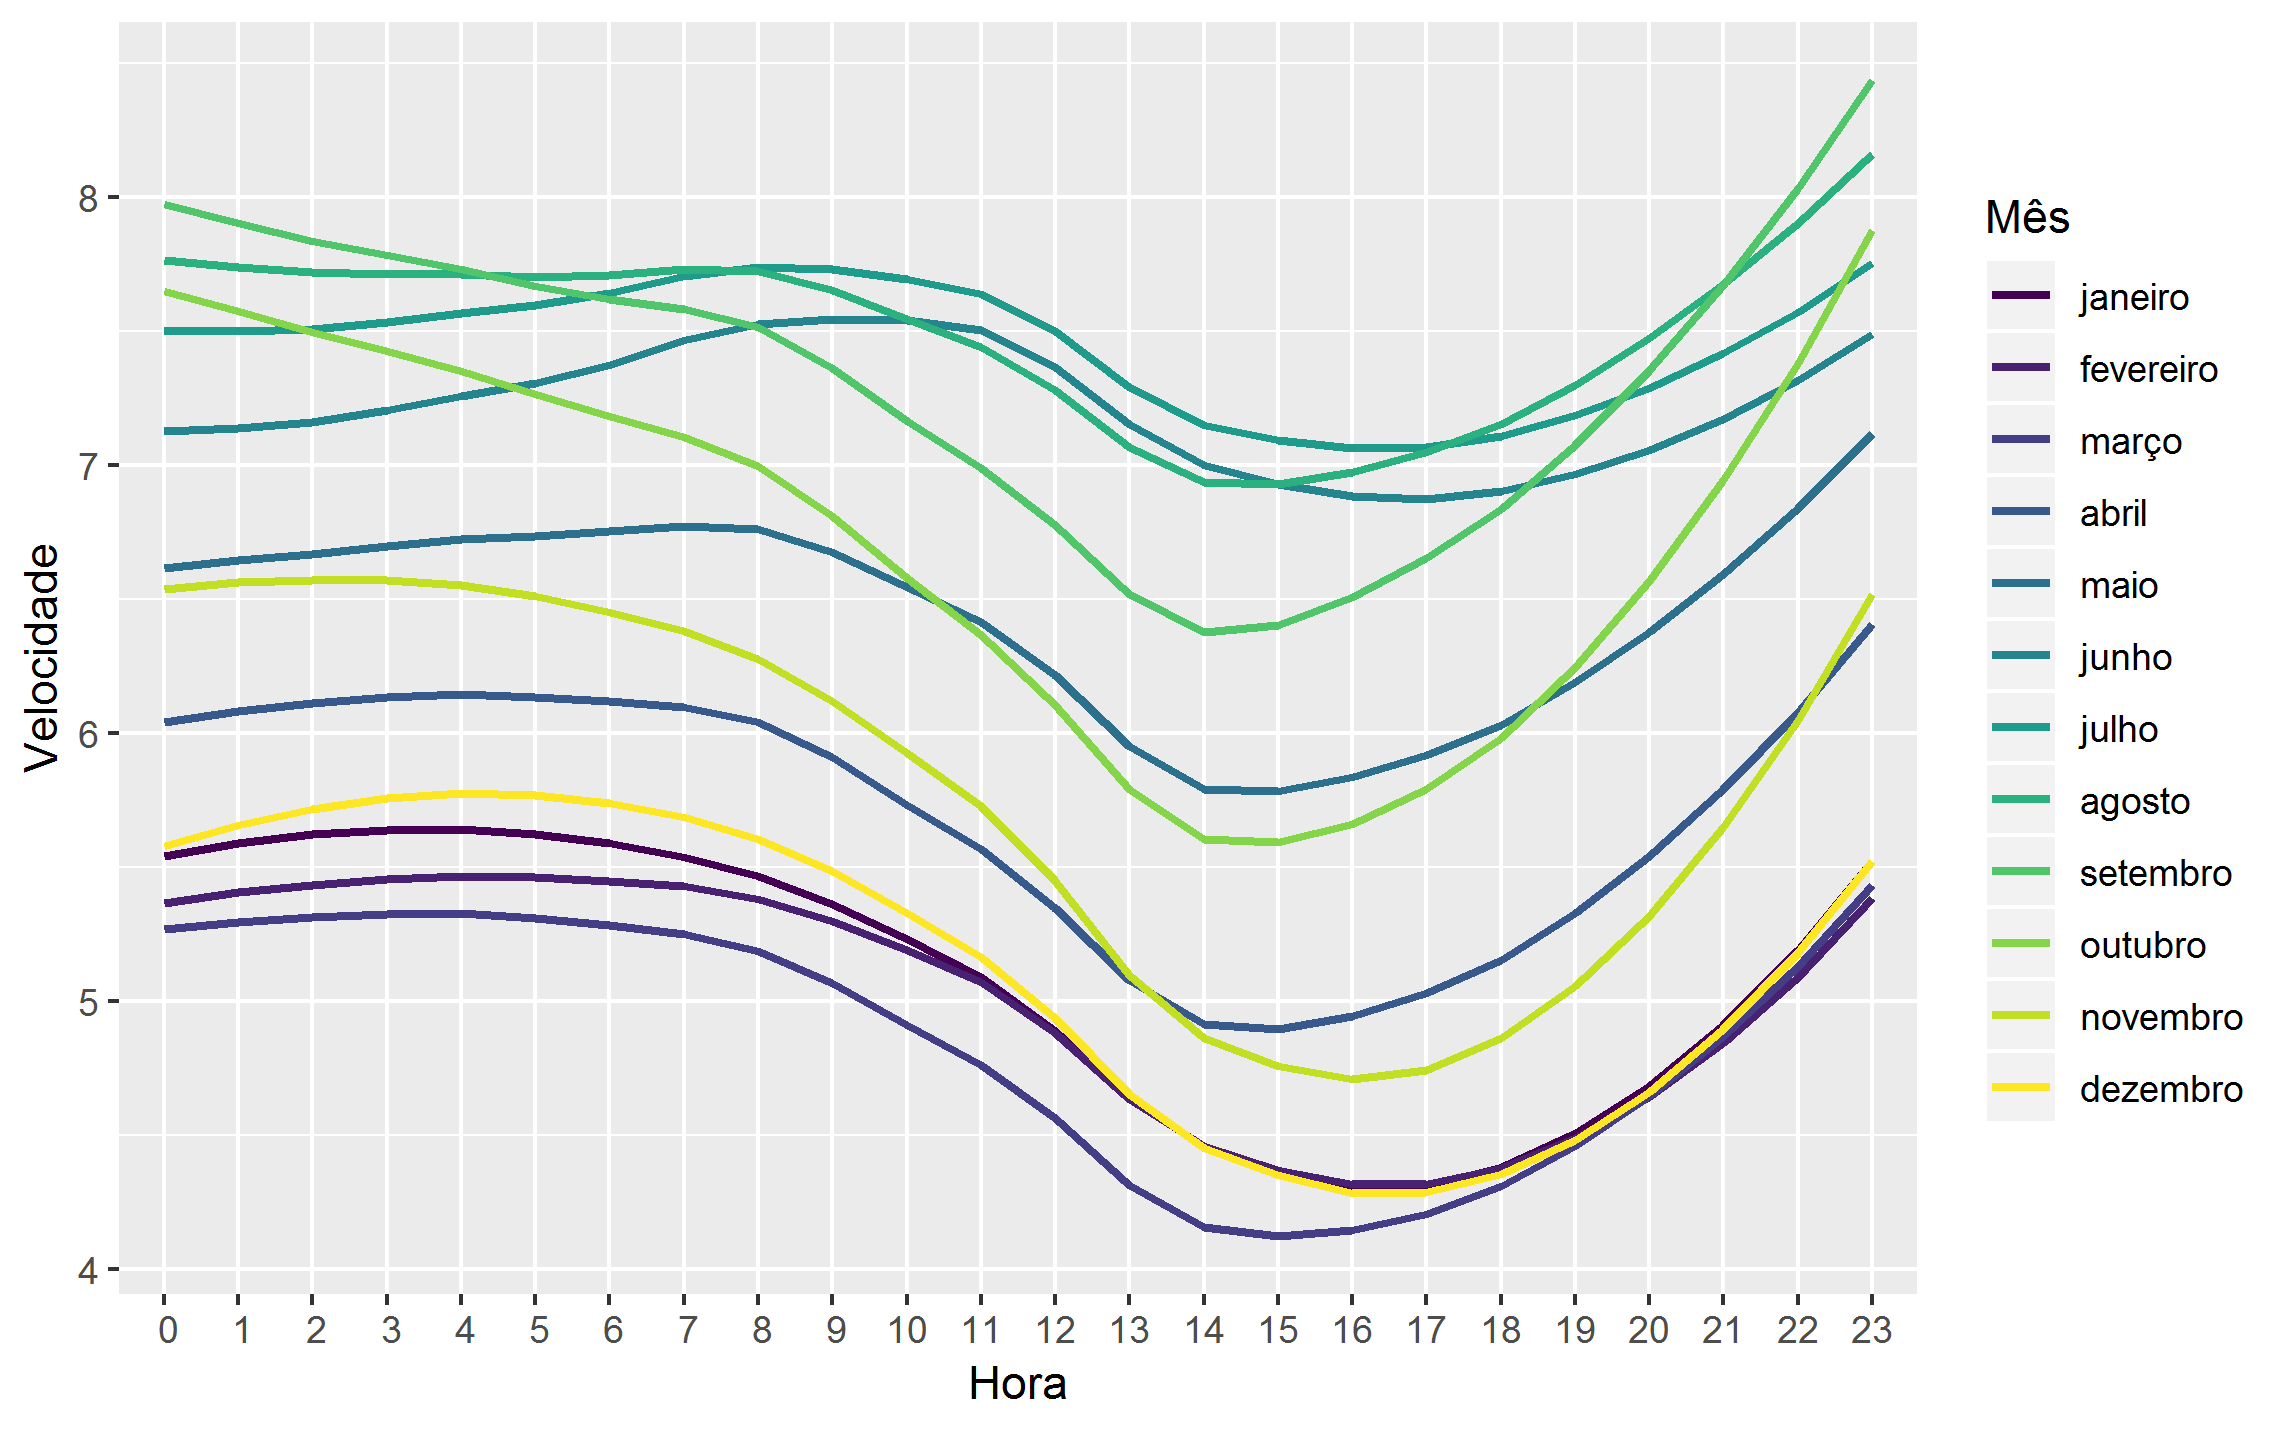
\includegraphics[scale=0.6]{diurnal}
%%		\caption{Evolução dos parâmetros p e q de um modelo ARIMA ao longo do tempo.}
	\end{figure}
\end{frame}

\begin{frame}
	\frametitle{GARCH}
	
	\begin{equation*}
		\sigma_t^2 = \underbrace{\beta_1\sigma_{t-1}^2 + \dots + \beta_p\sigma_{t-p}^2}_\text{autorregressão}  + \underbrace{\omega + \alpha_1\varepsilon_{t-1}^2 + \dots + \dots \alpha_q\varepsilon_{t-q}^2}_\text{média móvel} 
	\end{equation*}
	
	\begin{equation*}
		\sigma_t^2 = \sum\limits_{i=1}^q\beta_i\sigma_{t-i}^2 + \omega + \sum\limits_{i=1}^q\alpha_i\varepsilon_{t-i}^2
	\end{equation*}
\end{frame}
	
\begin{frame}
	\frametitle{GARCH: previsão em base horária}
	\begin{figure}
		\centering
		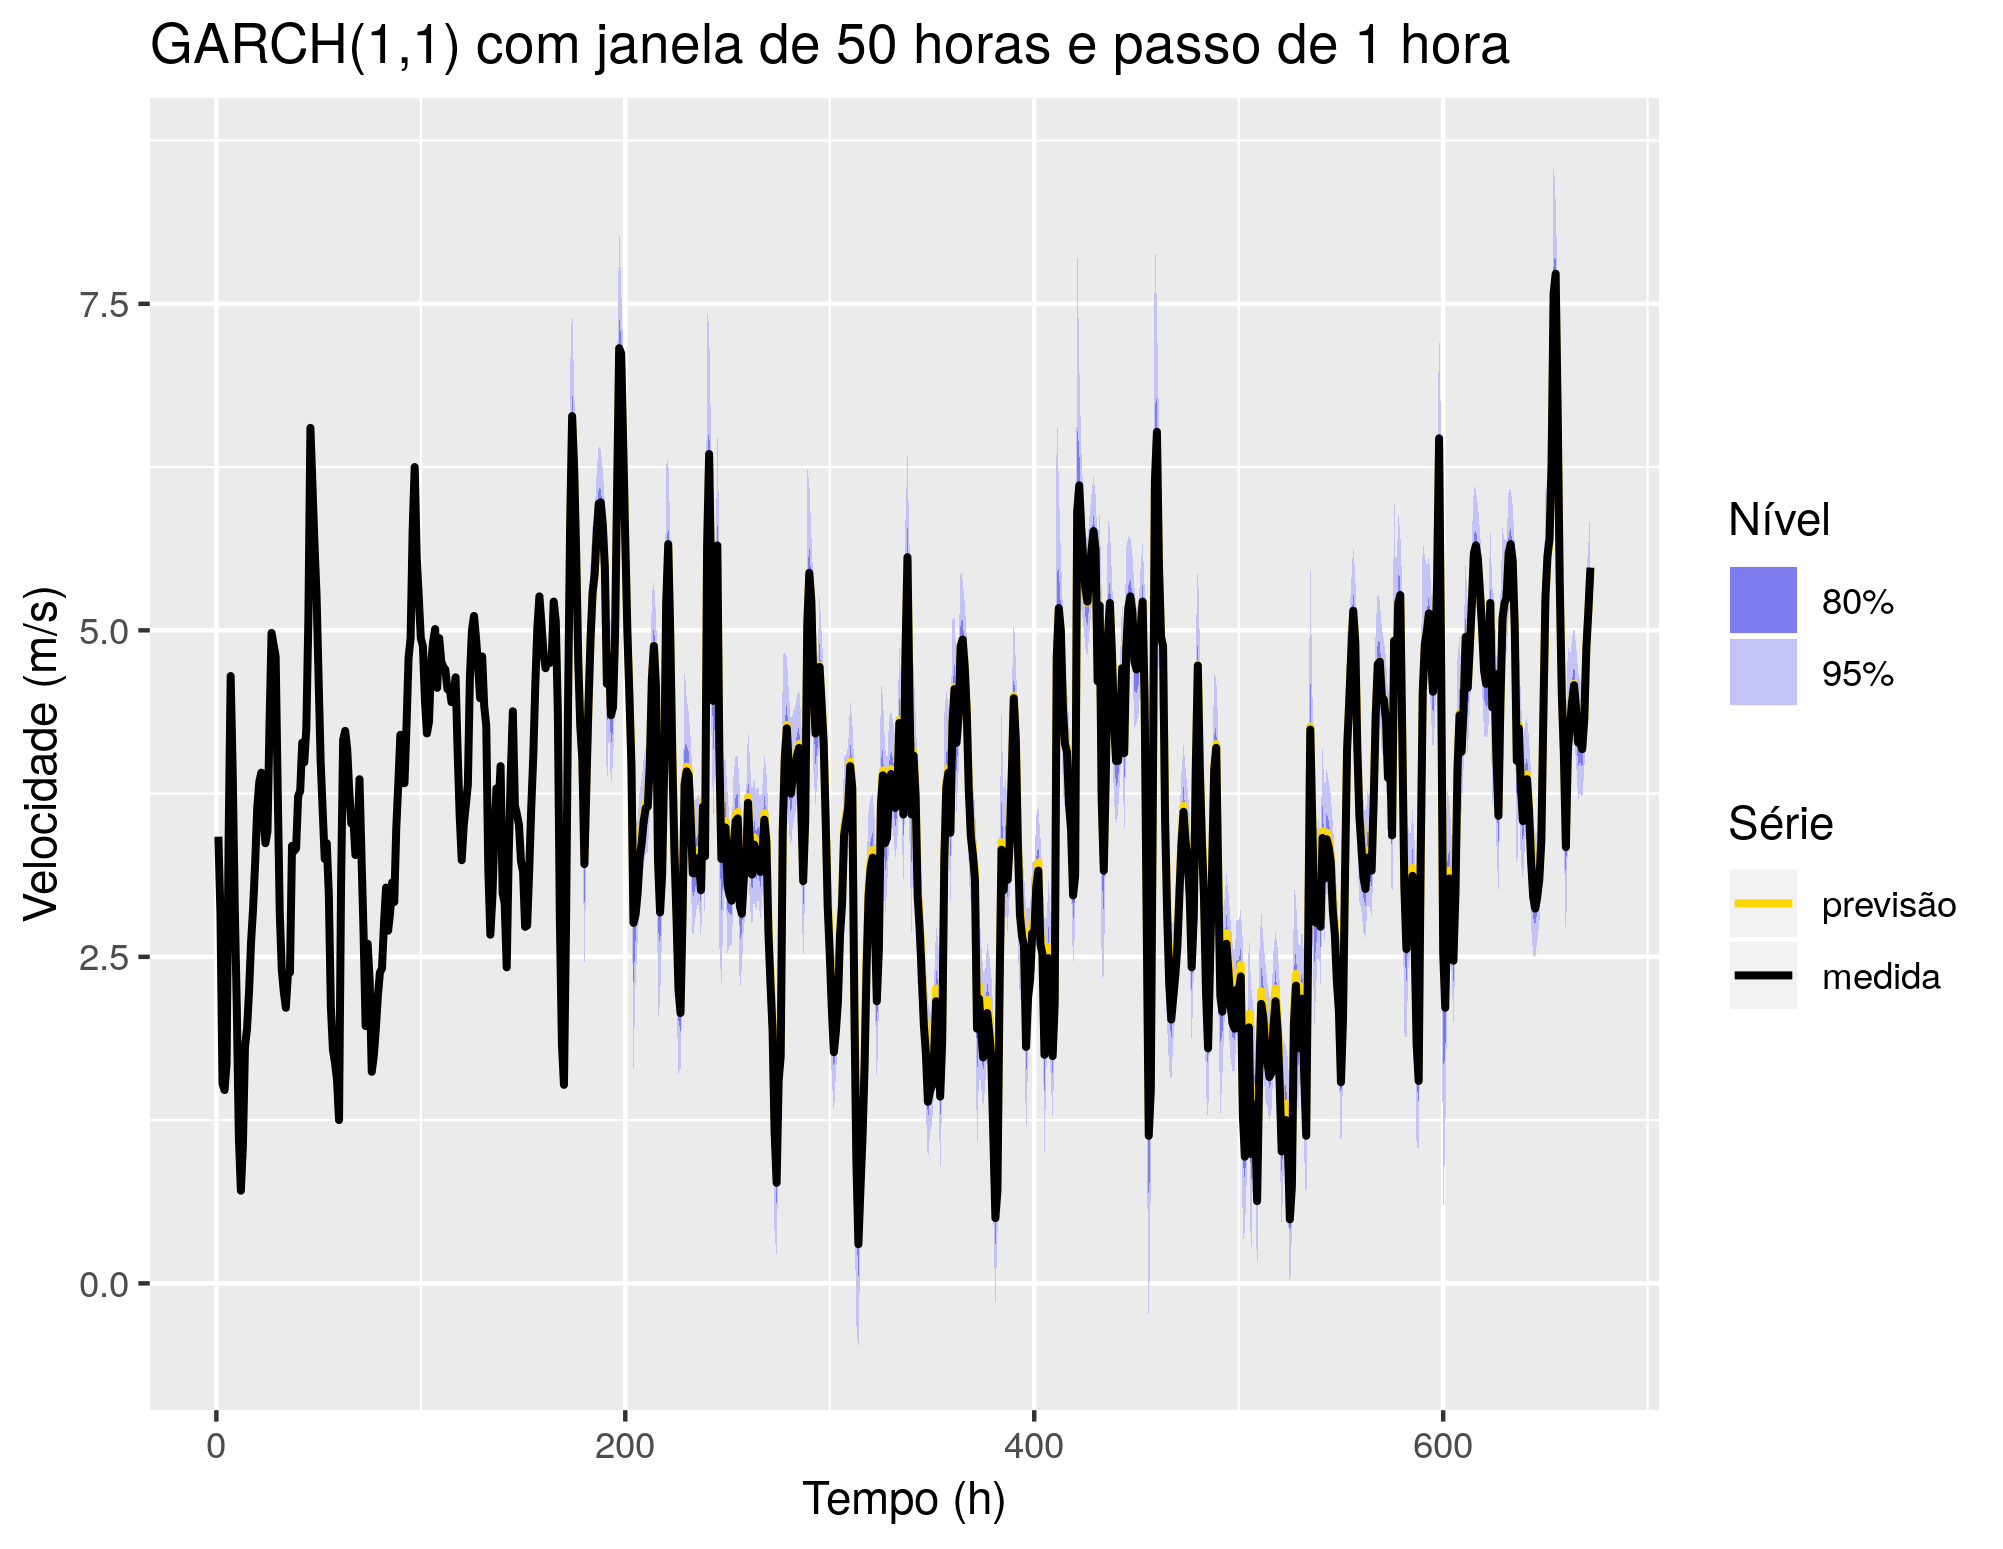
\includegraphics[scale=0.6]{garch_first}
%%		\caption{GARCH}
	\end{figure}
\end{frame}

\begin{frame}
	\frametitle{Comparação com resultados anteriores}

	\begin{table}[h]
		\centering
		\begin{tabular}{ |c|c|c|c|c|c| } 
			\hline
			\textbf{Modelo}&\textbf{ME}&\textbf{RMSE}&\textbf{MAE}&\textbf{MPE}&\textbf{MASE}\\
			\hline
			GARCH(1,1)&-0.042&0.065&0.051&-2.451&2.592 \\
			\hline
			ARIMA(1,1,1)&-0.008&0.223&0.162&0.382&5.731 \\
			\hline
			ARIMA(2,1,1)&0.008&0.297&0.228&-0.756&7.622 \\
			\hline
			ARIMA(1,1,2)&0.016&0.249&0.187&-0.839&6.152 \\
			\hline
			ARIMA(2,1,3)&0.0158&0.319&0.238&-0.838&7.968 \\
			\hline
		\end{tabular}
		\caption{Medidas de erro para 4 modelos ARIMA aplicados à séries modelo.}
	\end{table}
\end{frame}	
	
\begin{frame}
	\frametitle{GARCH: previsão em base mensal}
	\begin{figure}
		\centering
		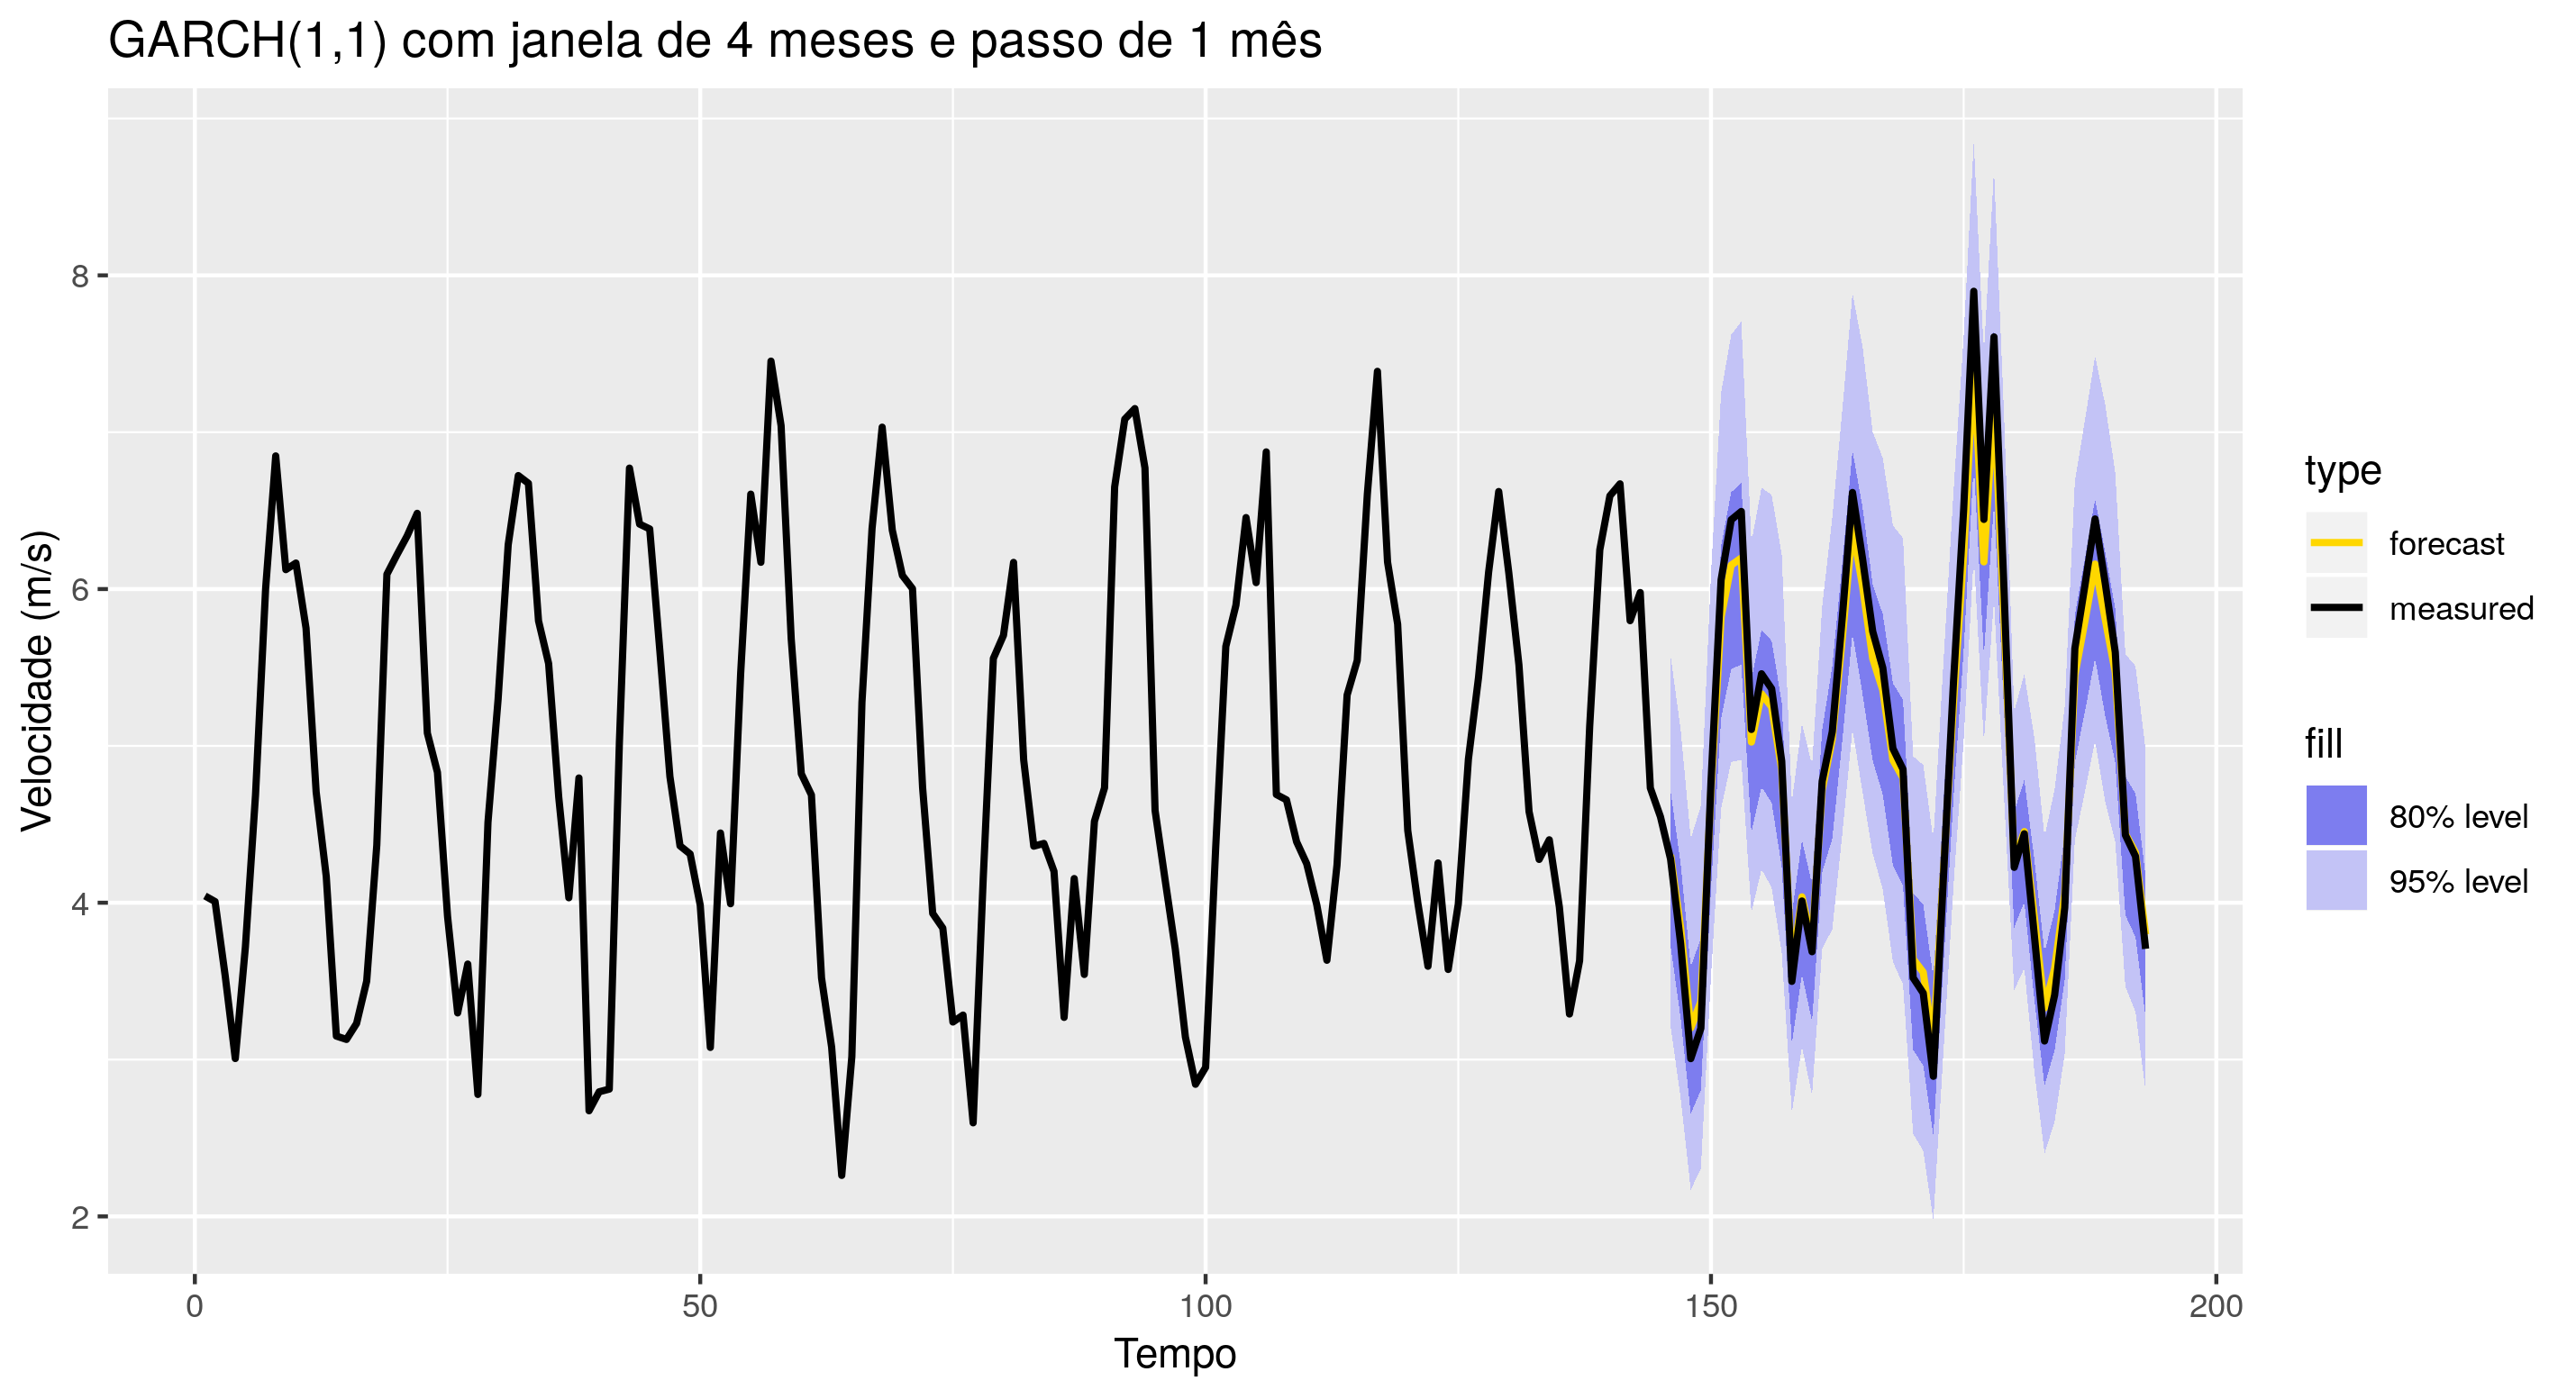
\includegraphics[width=\textwidth]{garch_month}
%%		\caption{GARCH}
	\end{figure}
\end{frame}

\section{Conclusão}

\subsection{Conversão em energia}

\begin{frame}
	\frametitle{O cálculo da potência}
	\begin{equation*}
		P = \frac{1}{2}\rho \frac{\pi D^2}{4}\nu^3C_p\eta
	\end{equation*}
	
	\begin{flalign*}
	P &= \mbox{potência elétrica na altura do cubo rotor}\left[W\right]&&\\
	\rho &= \mbox{densidade do ar}\left[\frac{kg}{m^3}\right]&&\\
	D &= \mbox{diâmetro do rotor}\left[m\right]&&\\\nonumber
	\nu &= \mbox{velocidade do vento} \left[\frac{m}{s}\right]&&\\\nonumber
	C_p &= \mbox{coeficiente aerodinâmico de potência do rotor}\left[W\right]&&\\\nonumber
	\eta &= \mbox{eficiência do conjunto gerador/transmissão}&&\\\nonumber
	\end{flalign*}
\end{frame}

\begin{frame}
	\frametitle{Curva de potência}
	\begin{figure}
		\centering
		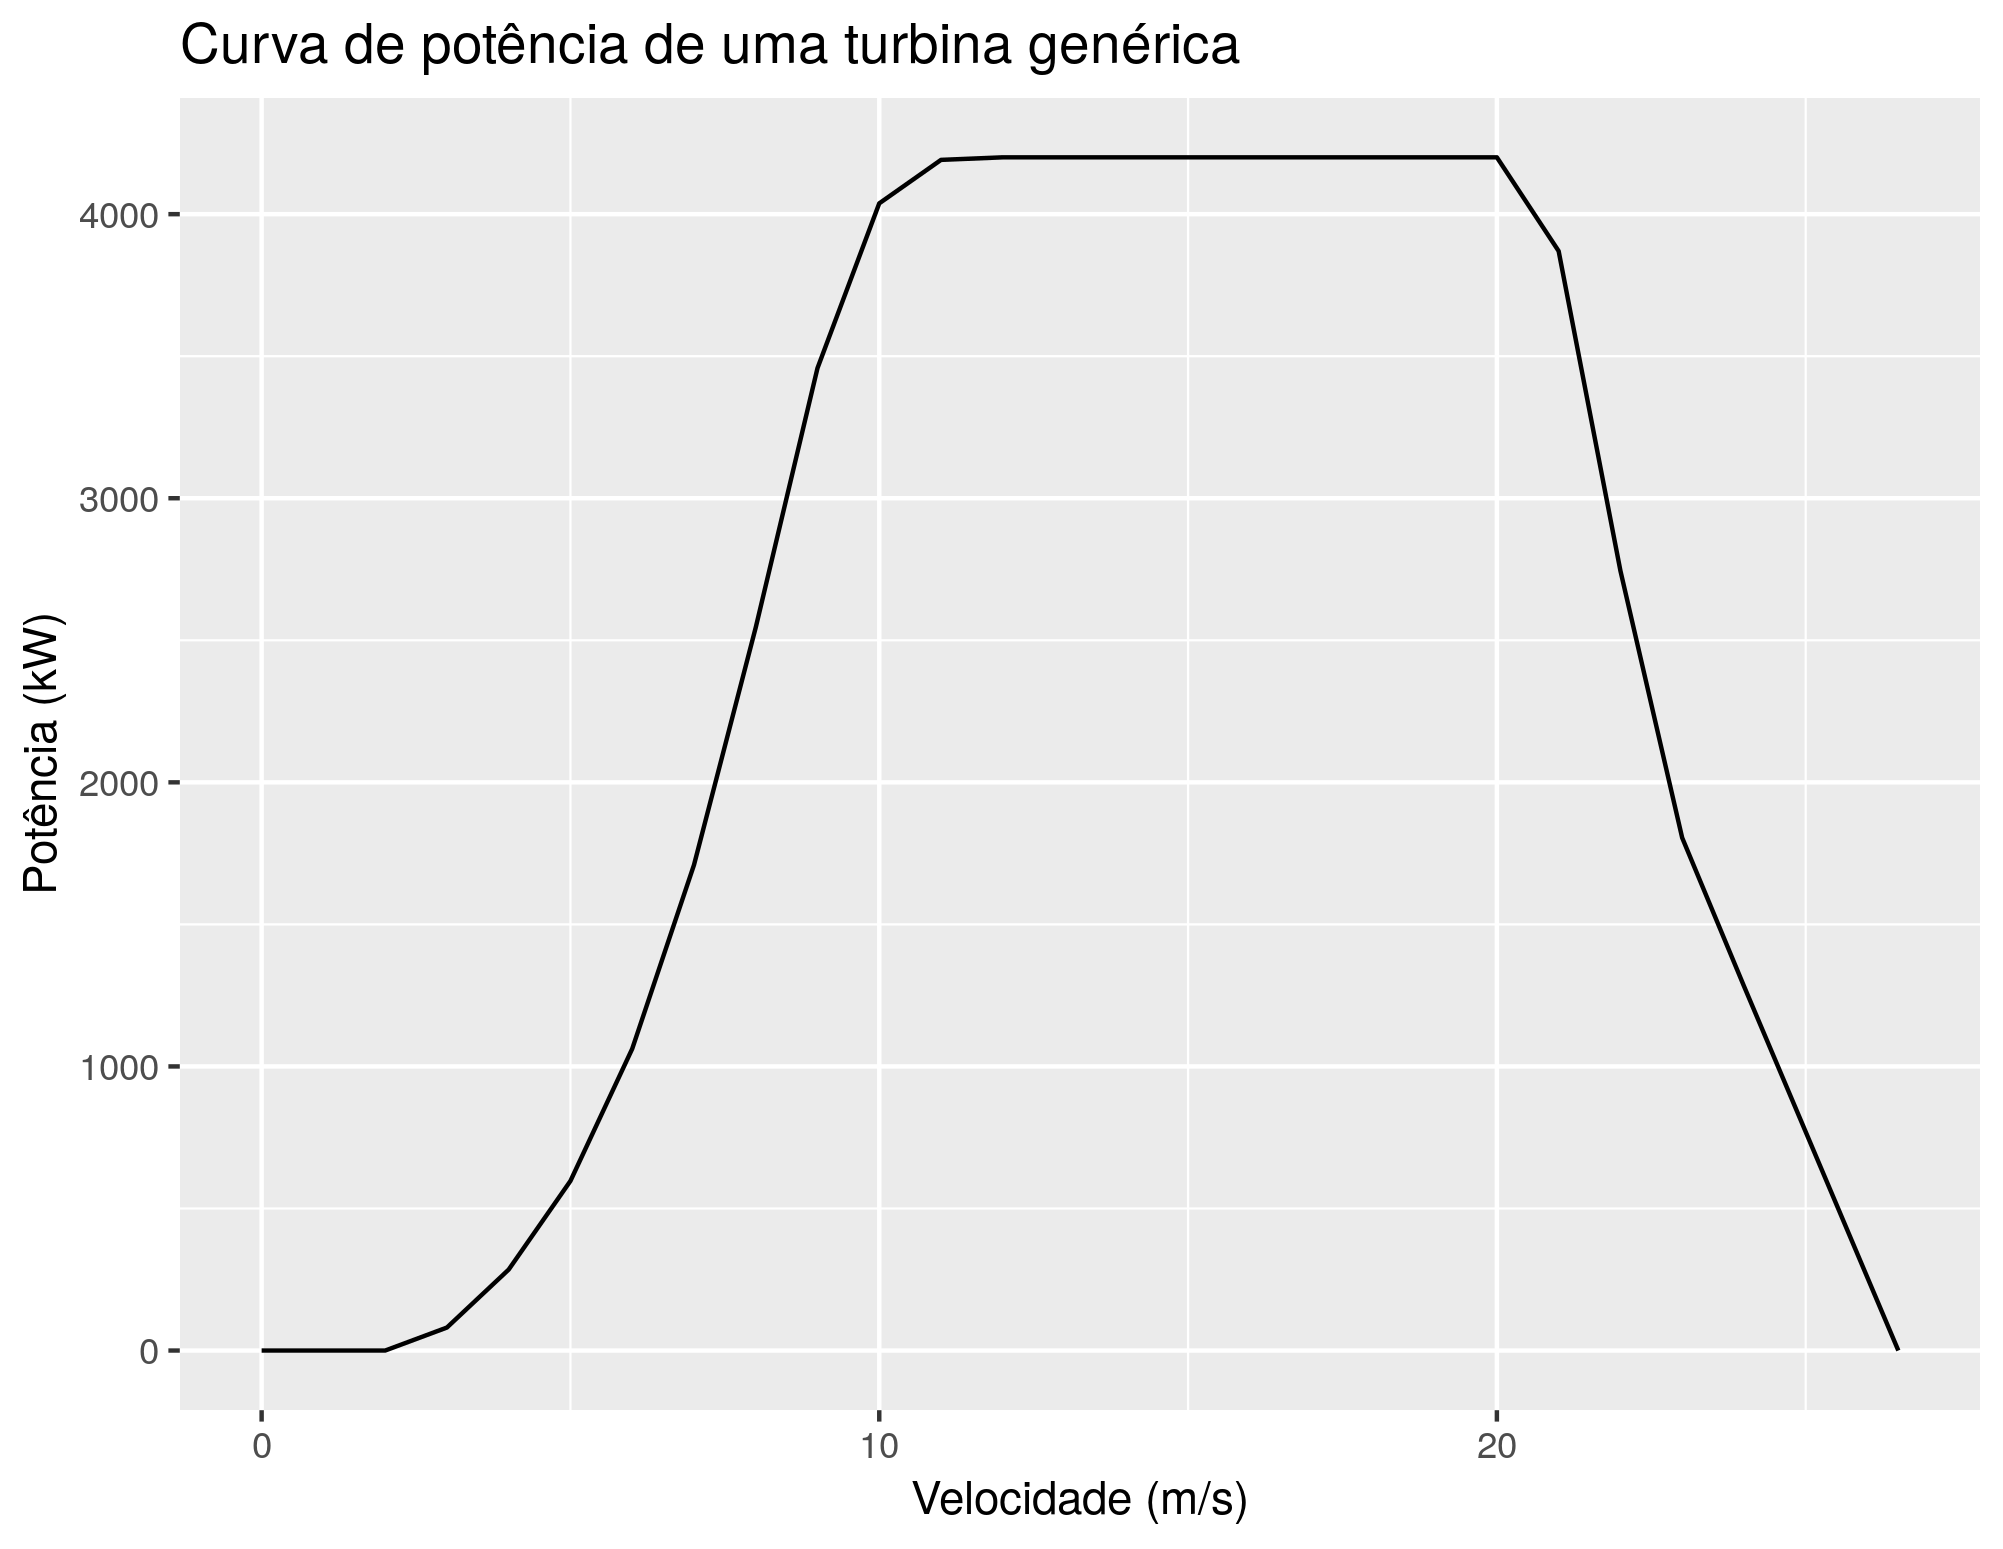
\includegraphics[scale=0.5]{power_curve}
%%		\caption{Curva de potência de um aerogerador genérico.}
	\end{figure}
\end{frame}

\begin{frame}
	\frametitle{Mapeamento entre velocidade e energia}
	\begin{figure}
		\centering
		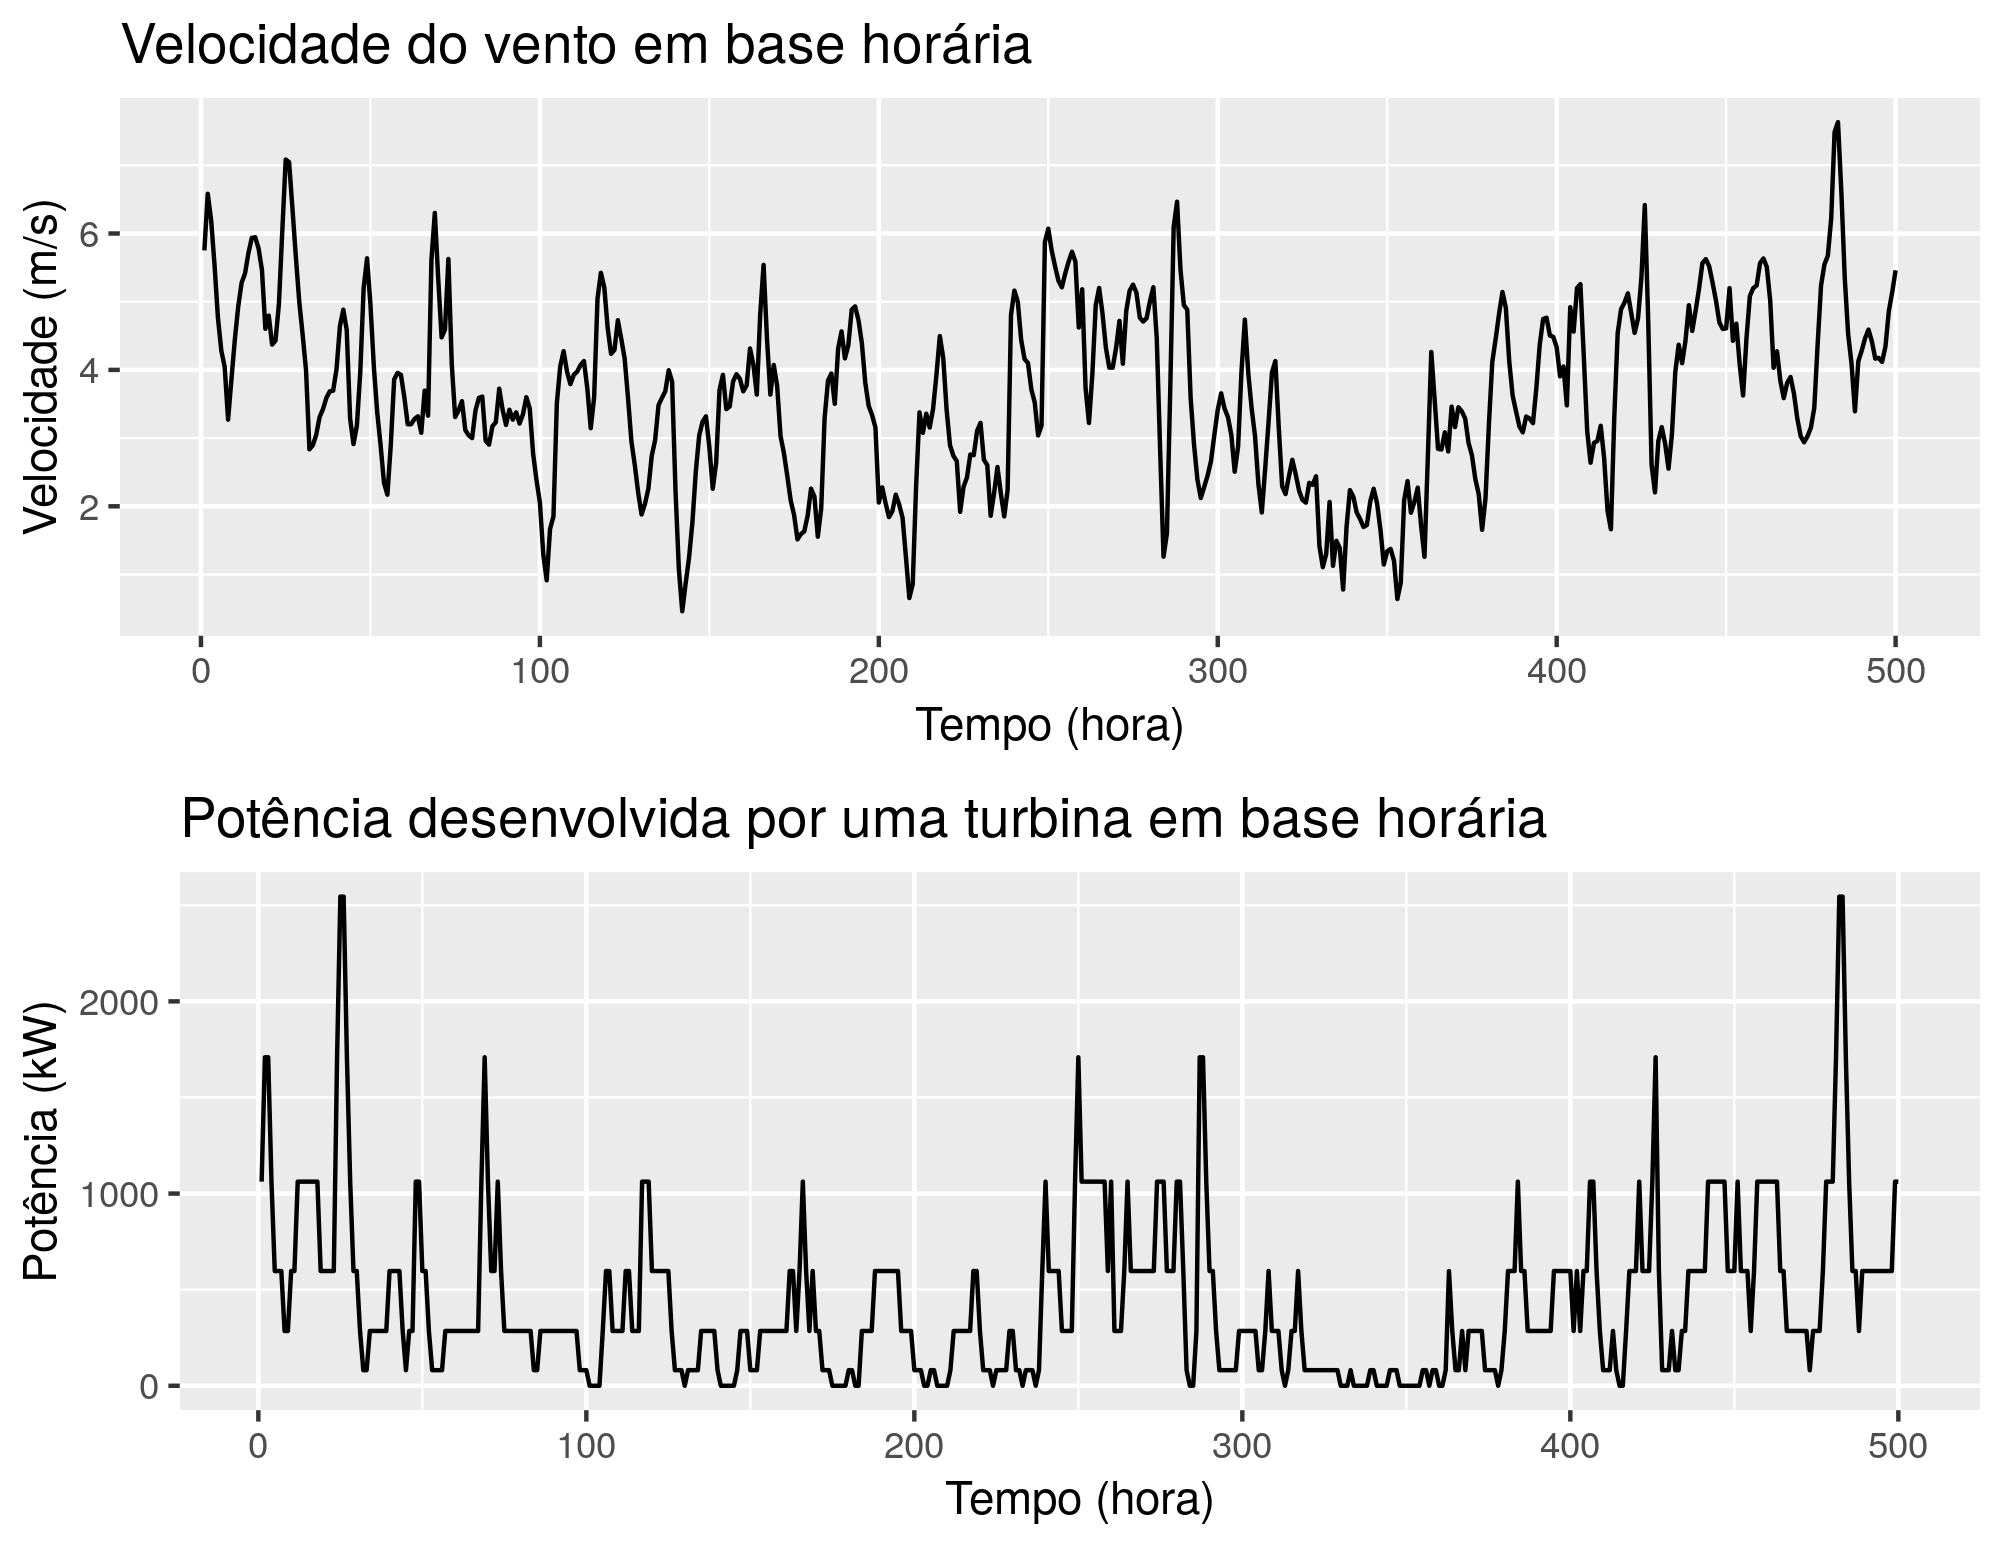
\includegraphics[scale=0.6]{speed_power}
%%		\caption{Curva de potência de um aerogerador genérico.}
	\end{figure}
\end{frame}

\begin{frame}
	\frametitle{Resultado e energia}
	\begin{alertblock}{500 horas de operação}
		\begin{itemize}
			\item Produção máxima: 2250 MWh
			\item Produção prevista: 217 MWh
			\item Produção real: 212 MWh
		\end{itemize}
	\end{alertblock}
	
	O MWh custa, atualmente, cerca de 180 reais (CCEE)
\end{frame}
	
\subsection{Validação com outras séries}

\begin{frame}
	\frametitle{Validação: diferentes regiões}
	\begin{figure}
		\centering
		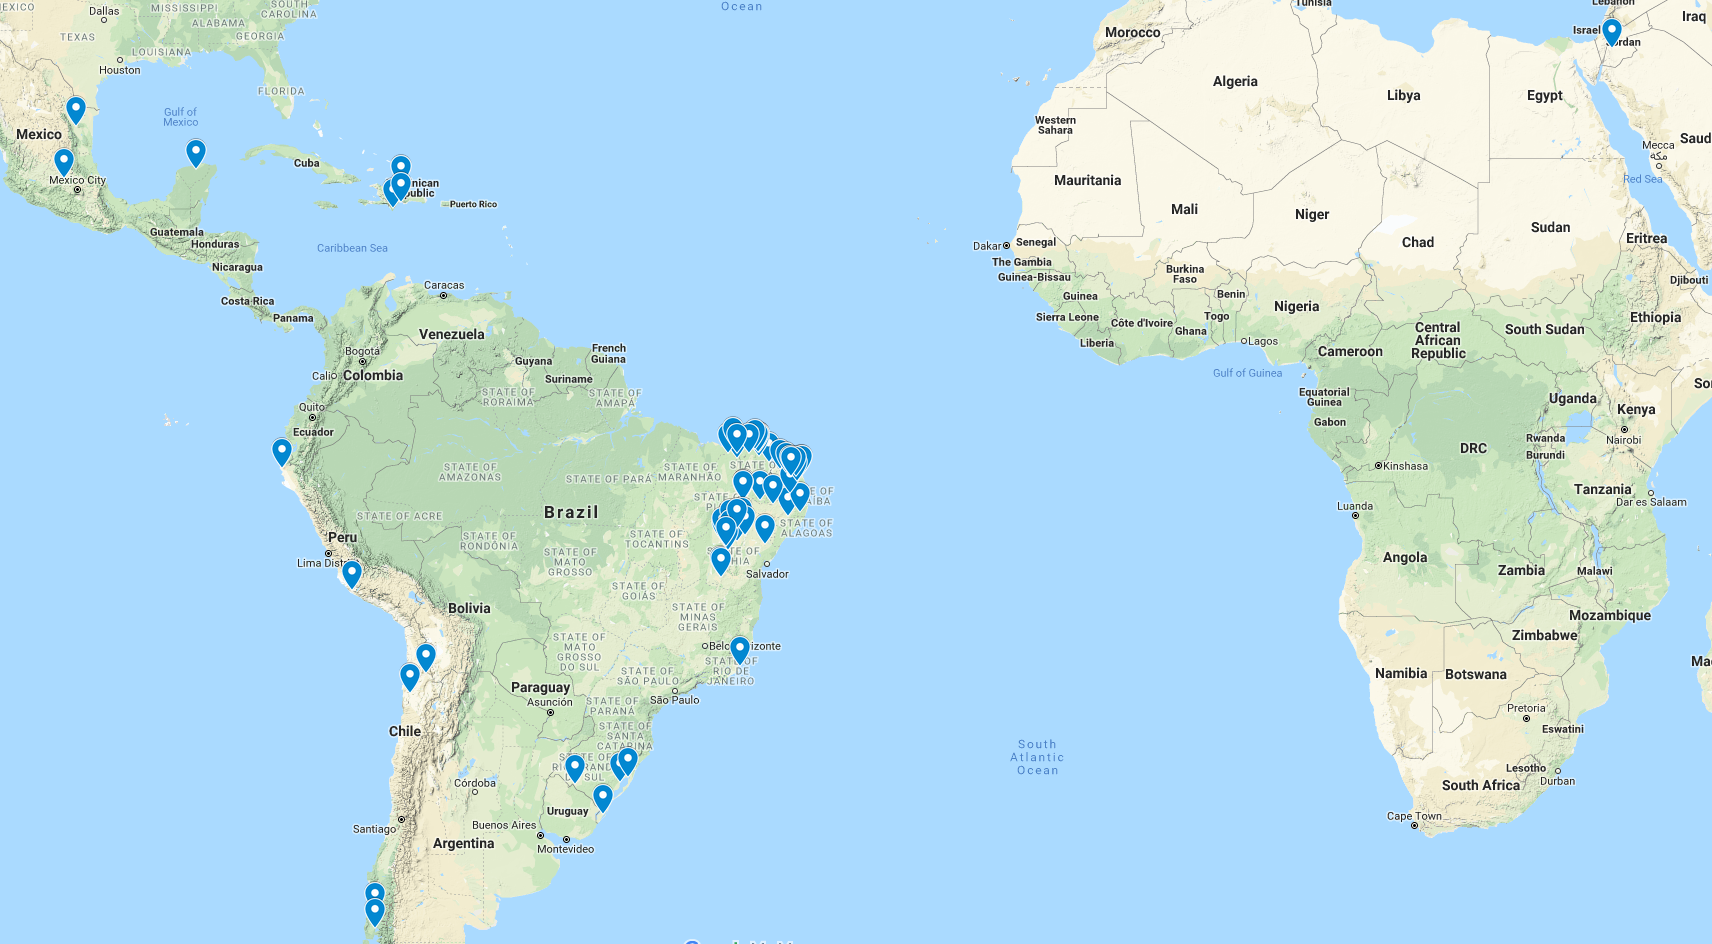
\includegraphics[width=\textwidth]{latam}
%%		\caption{TDEF Map}
	\end{figure}
\end{frame}

\begin{frame}
	\frametitle{Validação: melhores resultados}
	\begin{table}[h]
		\centering
		\begin{tabular}{ |c|c|c|c|c|c| } 
			\hline
			\textbf{Local}&\textbf{ME}&\textbf{RMSE}&\textbf{MAE}&\textbf{MPE}&\textbf{MASE}\\
			\hline
			NE01a&0.0&0.02&0.01&-0.0&0.17\\
			\hline
			NE05&0.01&0.02&0.01&0.02&0.17\\
			\hline
			ChapadaAraripe&0.01&0.02&0.01&0.02&0.17\\
			\hline
			Embuaca&-0.01&0.02&0.02&-0.16&0.27\\
			\hline
			Santos&-0.01&0.02&0.02&-0.16&0.27\\
			\hline
			LaGuajira&0.03&0.04&0.04&0.25&0.27\\
			\hline
			AsaBranca&0.02&0.03&0.02&0.19&0.28\\
			\hline
			Omega&0.02&0.03&0.03&0.14&0.28\\
			\hline
			Icarai&-0.01&0.02&0.02&-0.19&0.29\\
			\hline
			EsquinaDoVento&0.03&0.04&0.03&0.25&0.4\\
			\hline
		\end{tabular}
%		\caption{10 melhores localidades em relação a previsão com GARCH(1,1)}
	\end{table}
\end{frame}

\begin{frame}
	\frametitle{Validação: piores resultados}
	\begin{table}[h]
		\centering
		\begin{tabular}{ |c|c|c|c|c|c| } 
			\hline
			\textbf{Local}&\textbf{ME}&\textbf{RMSE}&\textbf{MAE}&\textbf{MPE}&\textbf{MASE}\\
			\hline
			Omega\_RJ&0.1&0.13&0.11&1.48&2.02\\
			\hline
			Ibipeba&-0.04&0.07&0.05&-1.83&2.11\\
			\hline
			Tafila\_ERA5&0.05&0.11&0.08&-0.19&2.33\\
			\hline
			CapaoAlto&0.0&0.07&0.06&-1.63&2.41\\
			\hline
			Quadran&-0.05&0.07&0.05&-2.48&2.61\\
			\hline
			LaVigia&-0.01&0.06&0.05&-2.28&3.12\\
			\hline
			Ckani&0.05&0.13&0.09&-0.95&3.35\\
			\hline
			SanPedro&0.08&0.17&0.12&-0.1&3.94\\
			\hline
			Tucano&-0.05&0.15&0.13&-3.74&4.8\\
			\hline
			Llanos&0.22&0.33&0.24&3.47&12.58\\
			\hline
		\end{tabular}
%		\caption{10 piores localidades em relação a previsão com GARCH(1,1)}
	\end{table}
\end{frame}


%#***********
%#* TDEF I: *    
%#***********

%    \AtBeginSection[]
%    {
%      \begin{frame}
%        \frametitle{Sumário}
%        \tableofcontents[currentsection]
%      \end{frame}
%    }
%    
%    \AtBeginSubsection[]
%    {
%      \begin{frame}
%        \frametitle{Sumário}
%        \tableofcontents[currentsection,currentsubsection]
%      \end{frame}
%    }

%{ 
%\usebackgroundtemplate{\includegraphics[width=\paperwidth,height=\paperheight]{osorio}} 


%\frame
%{
%	\frametitle{Energia eólica}        
%	O investimento em energia eólica vem crescendo em todo o mundo:\newline        
%	\begin{itemize}
%        \item Alternativa a fontes de energia não-renováveis
%        \item Capaz de suprir boa parte da demanda de um país
%        \item Economicamente viável
%        \item Décadas de experiência acumulada
%	\end{itemize}
%}

%\frame
%{
%	\frametitle{Energia eólica: em crescimento}
%	\begin{figure}[h]
%   \centering
%	\includegraphics[scale=0.47]{19802010}
%	\caption{Geração de energia. Fonte: EPE.}
%	\end{figure}
%}

%\frame
%{
%	\frametitle{O recurso eólico nacional}
%	\begin{figure}[h]
%   	\centering
%		\includegraphics[scale=0.5]{brasilpotencialeolico}
%%%		\caption{O potencial eólico do Brasil. Fonte: CEPEL.}
%	\end{figure}
%}

%\frame
%{
%	\frametitle{O cálculo da potência}
%	\begin{equation*}
%		P = \frac{1}{2}\rho \frac{\pi D^2}{4}\nu^3C_p\eta
%	\end{equation*}
%	
%	\begin{flalign*}
%	P &= \mbox{potência elétrica na altura do cubo rotor}\left[W\right]&&\\
%	\rho &= \mbox{densidade do ar}\left[\frac{kg}{m^3}\right]&&\\
%	D &= \mbox{diâmetro do rotor}\left[m\right]&&\\\nonumber
%	\nu &= \mbox{velocidade do vento} \left[\frac{m}{s}\right]&&\\\nonumber
%	C_p &= \mbox{coeficiente aerodinâmico de potência do rotor}\left[W\right]&&\\\nonumber
%	\eta &= \mbox{eficiência do conjunto gerador/transmissão}&&\\\nonumber
%	\end{flalign*}
%}

%\frame
%{
%	\frametitle{Consumo médio residencial}
%	\begin{figure}[h]
%    	\centering
%		\includegraphics[width=\textwidth]{consumoresidencial}
%%%		\caption{Consumo médio residencial no país. Fonte: EPE.}
%	\end{figure}
%}

%\frame
%{
%	\frametitle{Dados de vento ERA 5: cidade de Sento Sé}
%	\begin{figure}[h]
%   	\centering
%		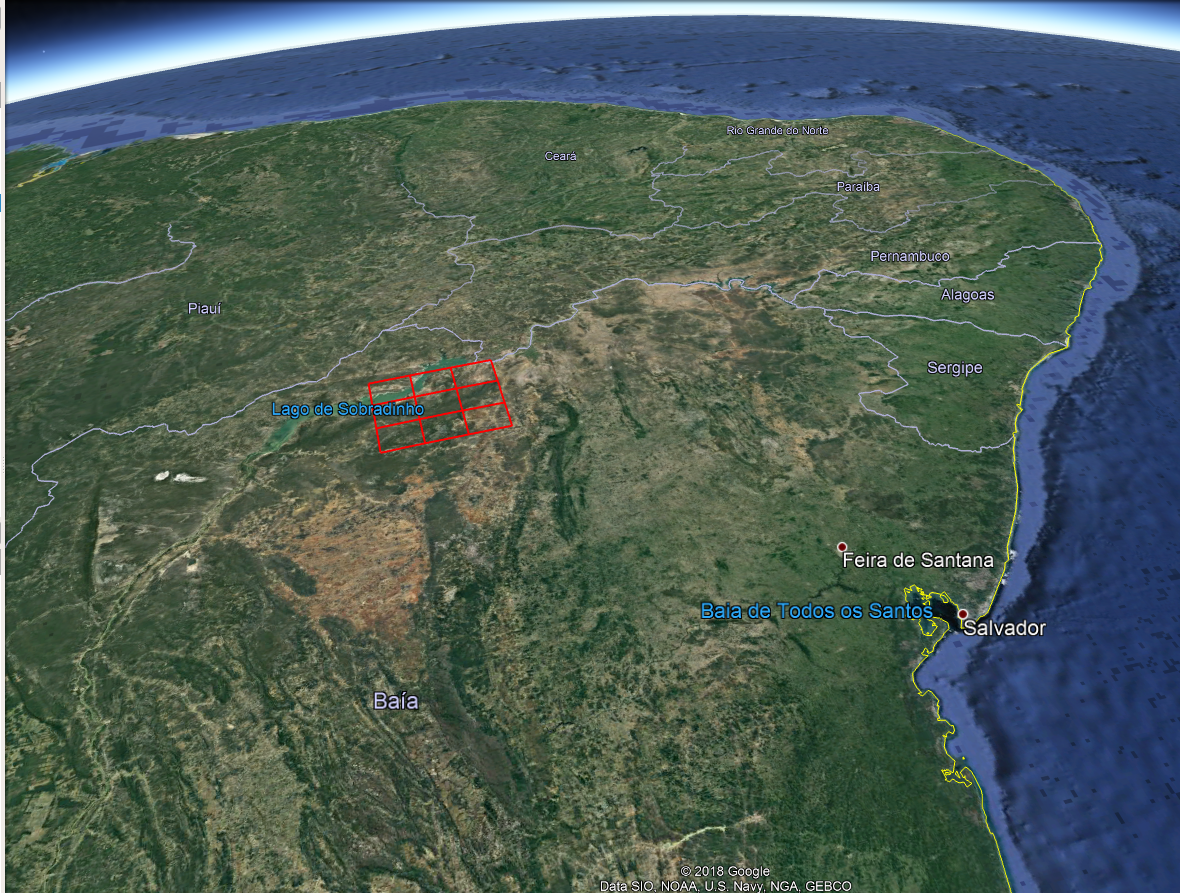
\includegraphics[width=\textwidth]{earth}
%%%		\caption{Localização da região de medição por satélite da cidade de Sento Sé. Fonte: SIO, NOAA, U.S. Navy, NGA, GEBCO. \textcopyright \  2018 Google}
%	\end{figure}
%}

%\frame
%{
%	\frametitle{Rosa dos ventos anual}
%	\begin{figure}[h]
 %   	\centering
%		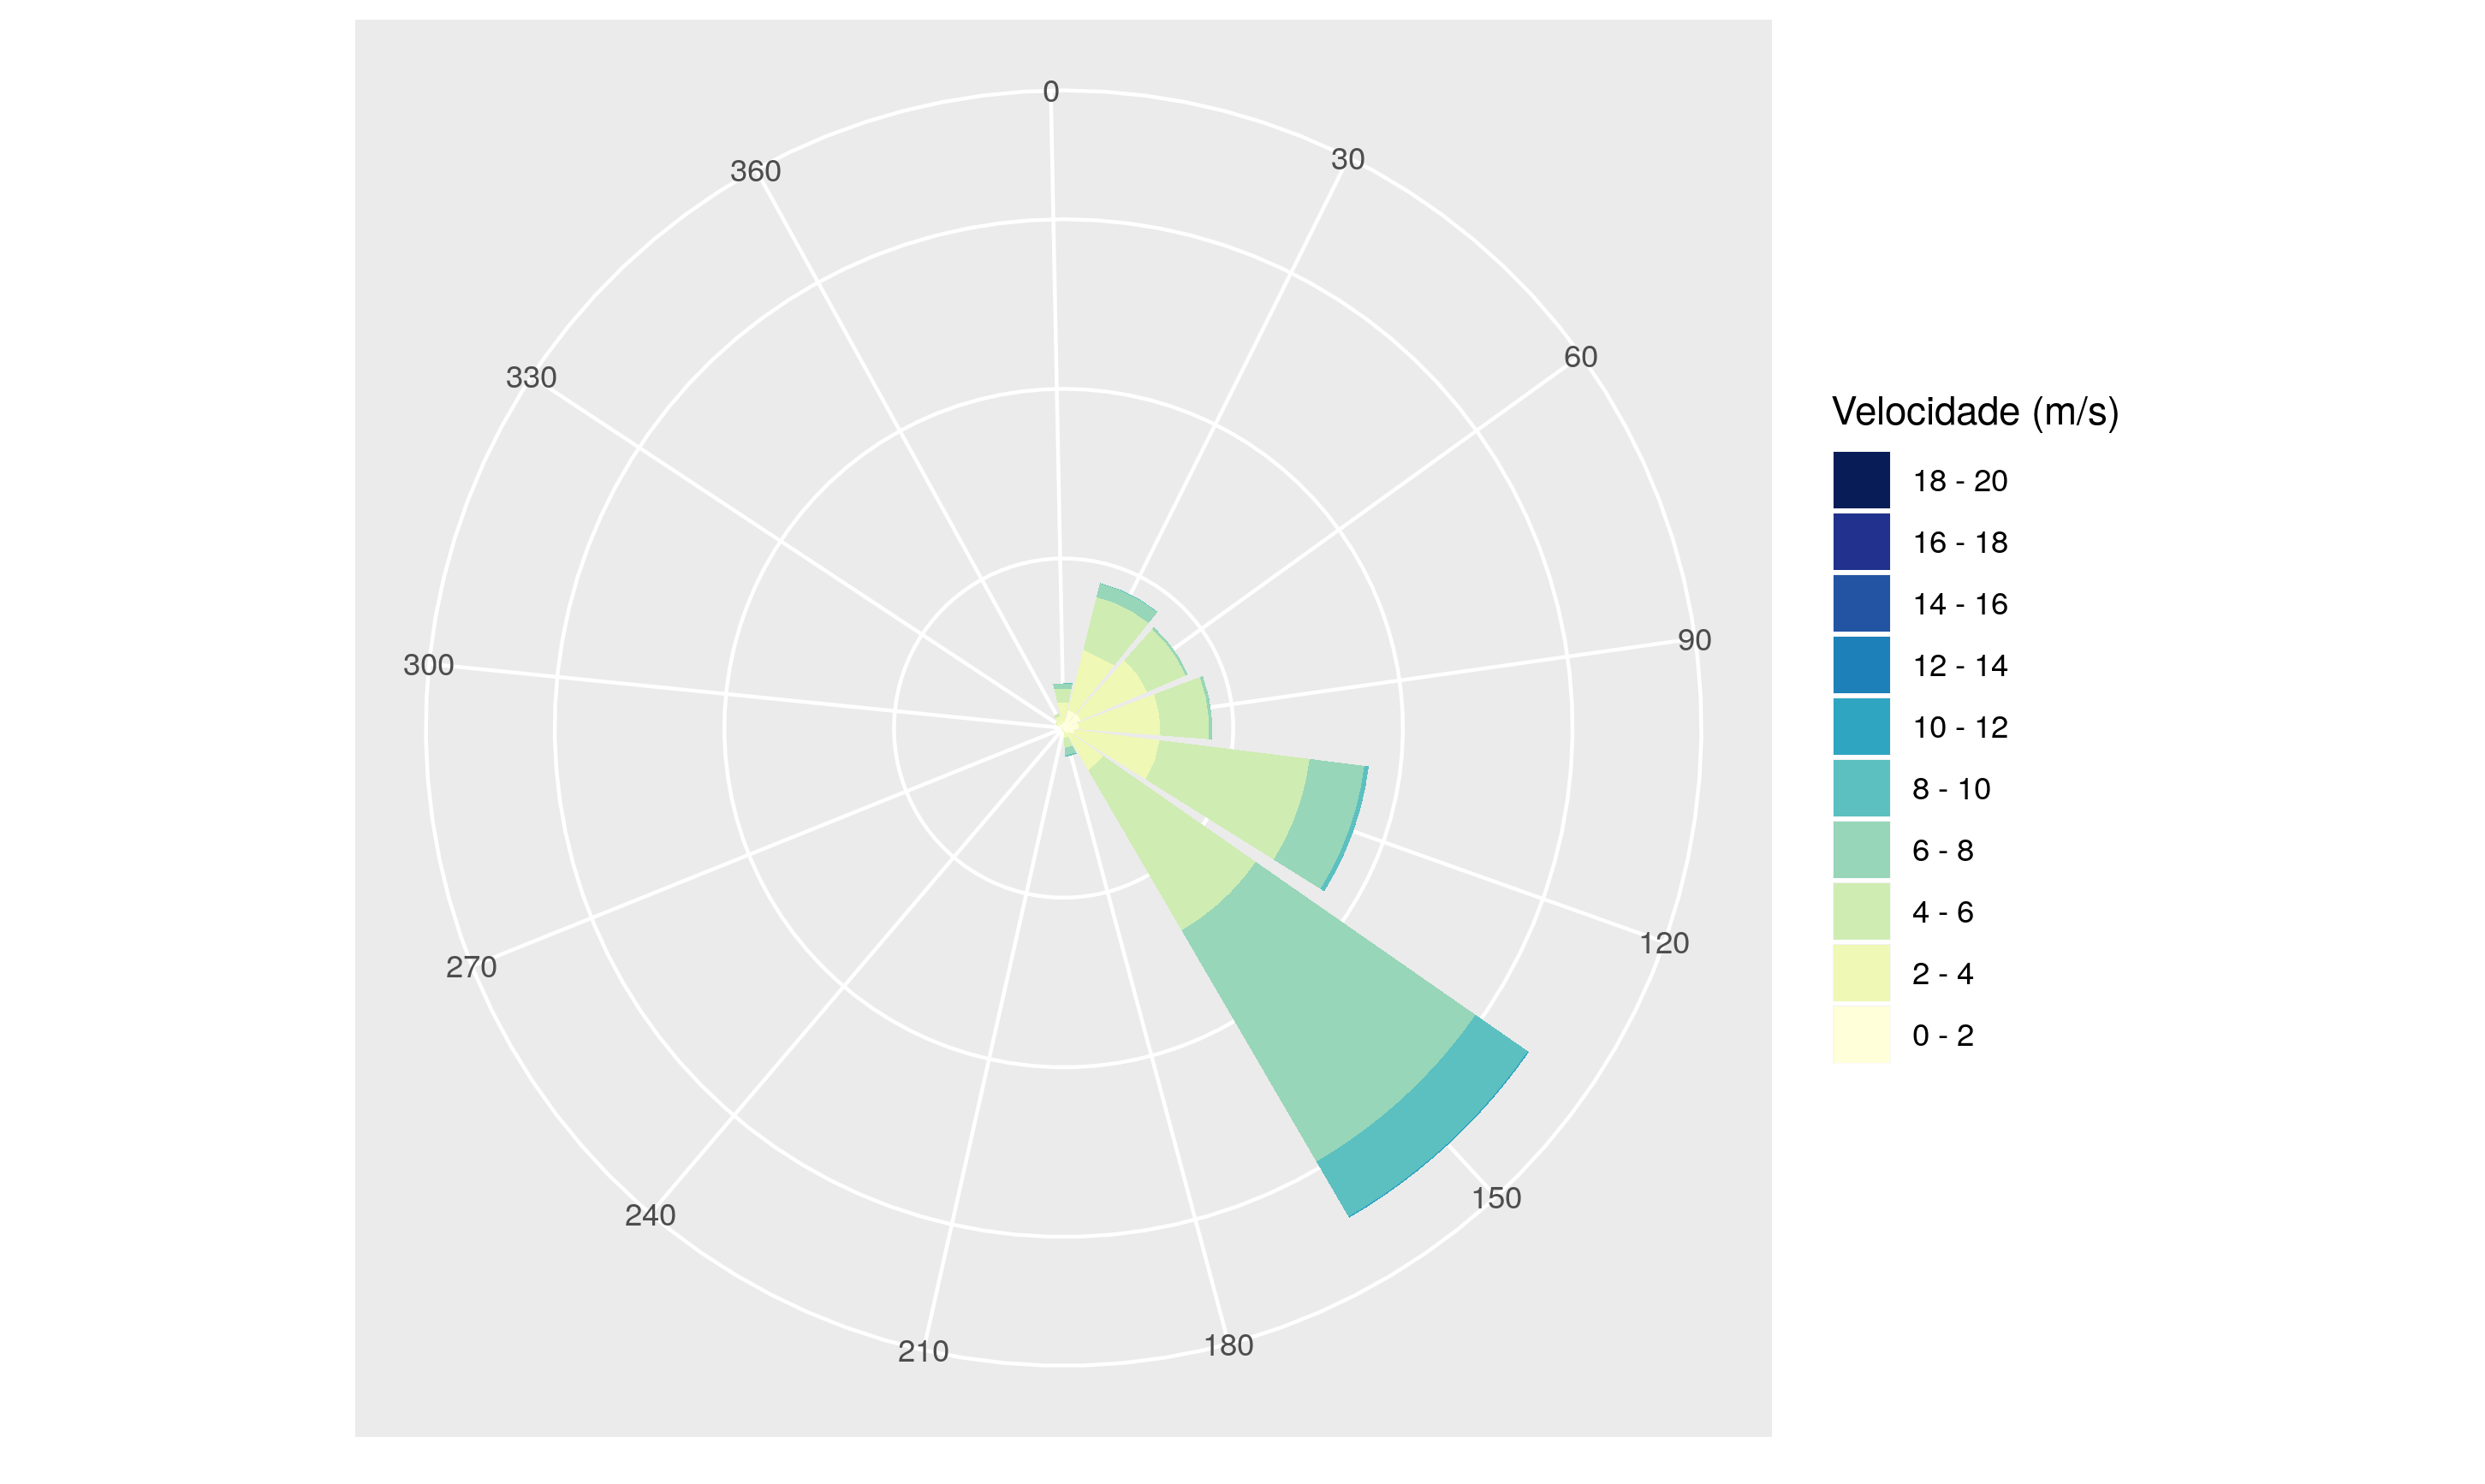
\includegraphics[scale=0.55]{windrose}
%%%		\caption{Rosa dos ventos do recurso eólico da cidade de Sento Sé no norte da Bahia. Fonte: autoria própria, dados: ECWMF.}
%	\end{figure}
%}

%\frame
%{
%	\frametitle{Rosas dos ventos mensais}
%	\begin{figure}[h]
%    	\centering
%  		\hspace*{-1.4cm}   
%   	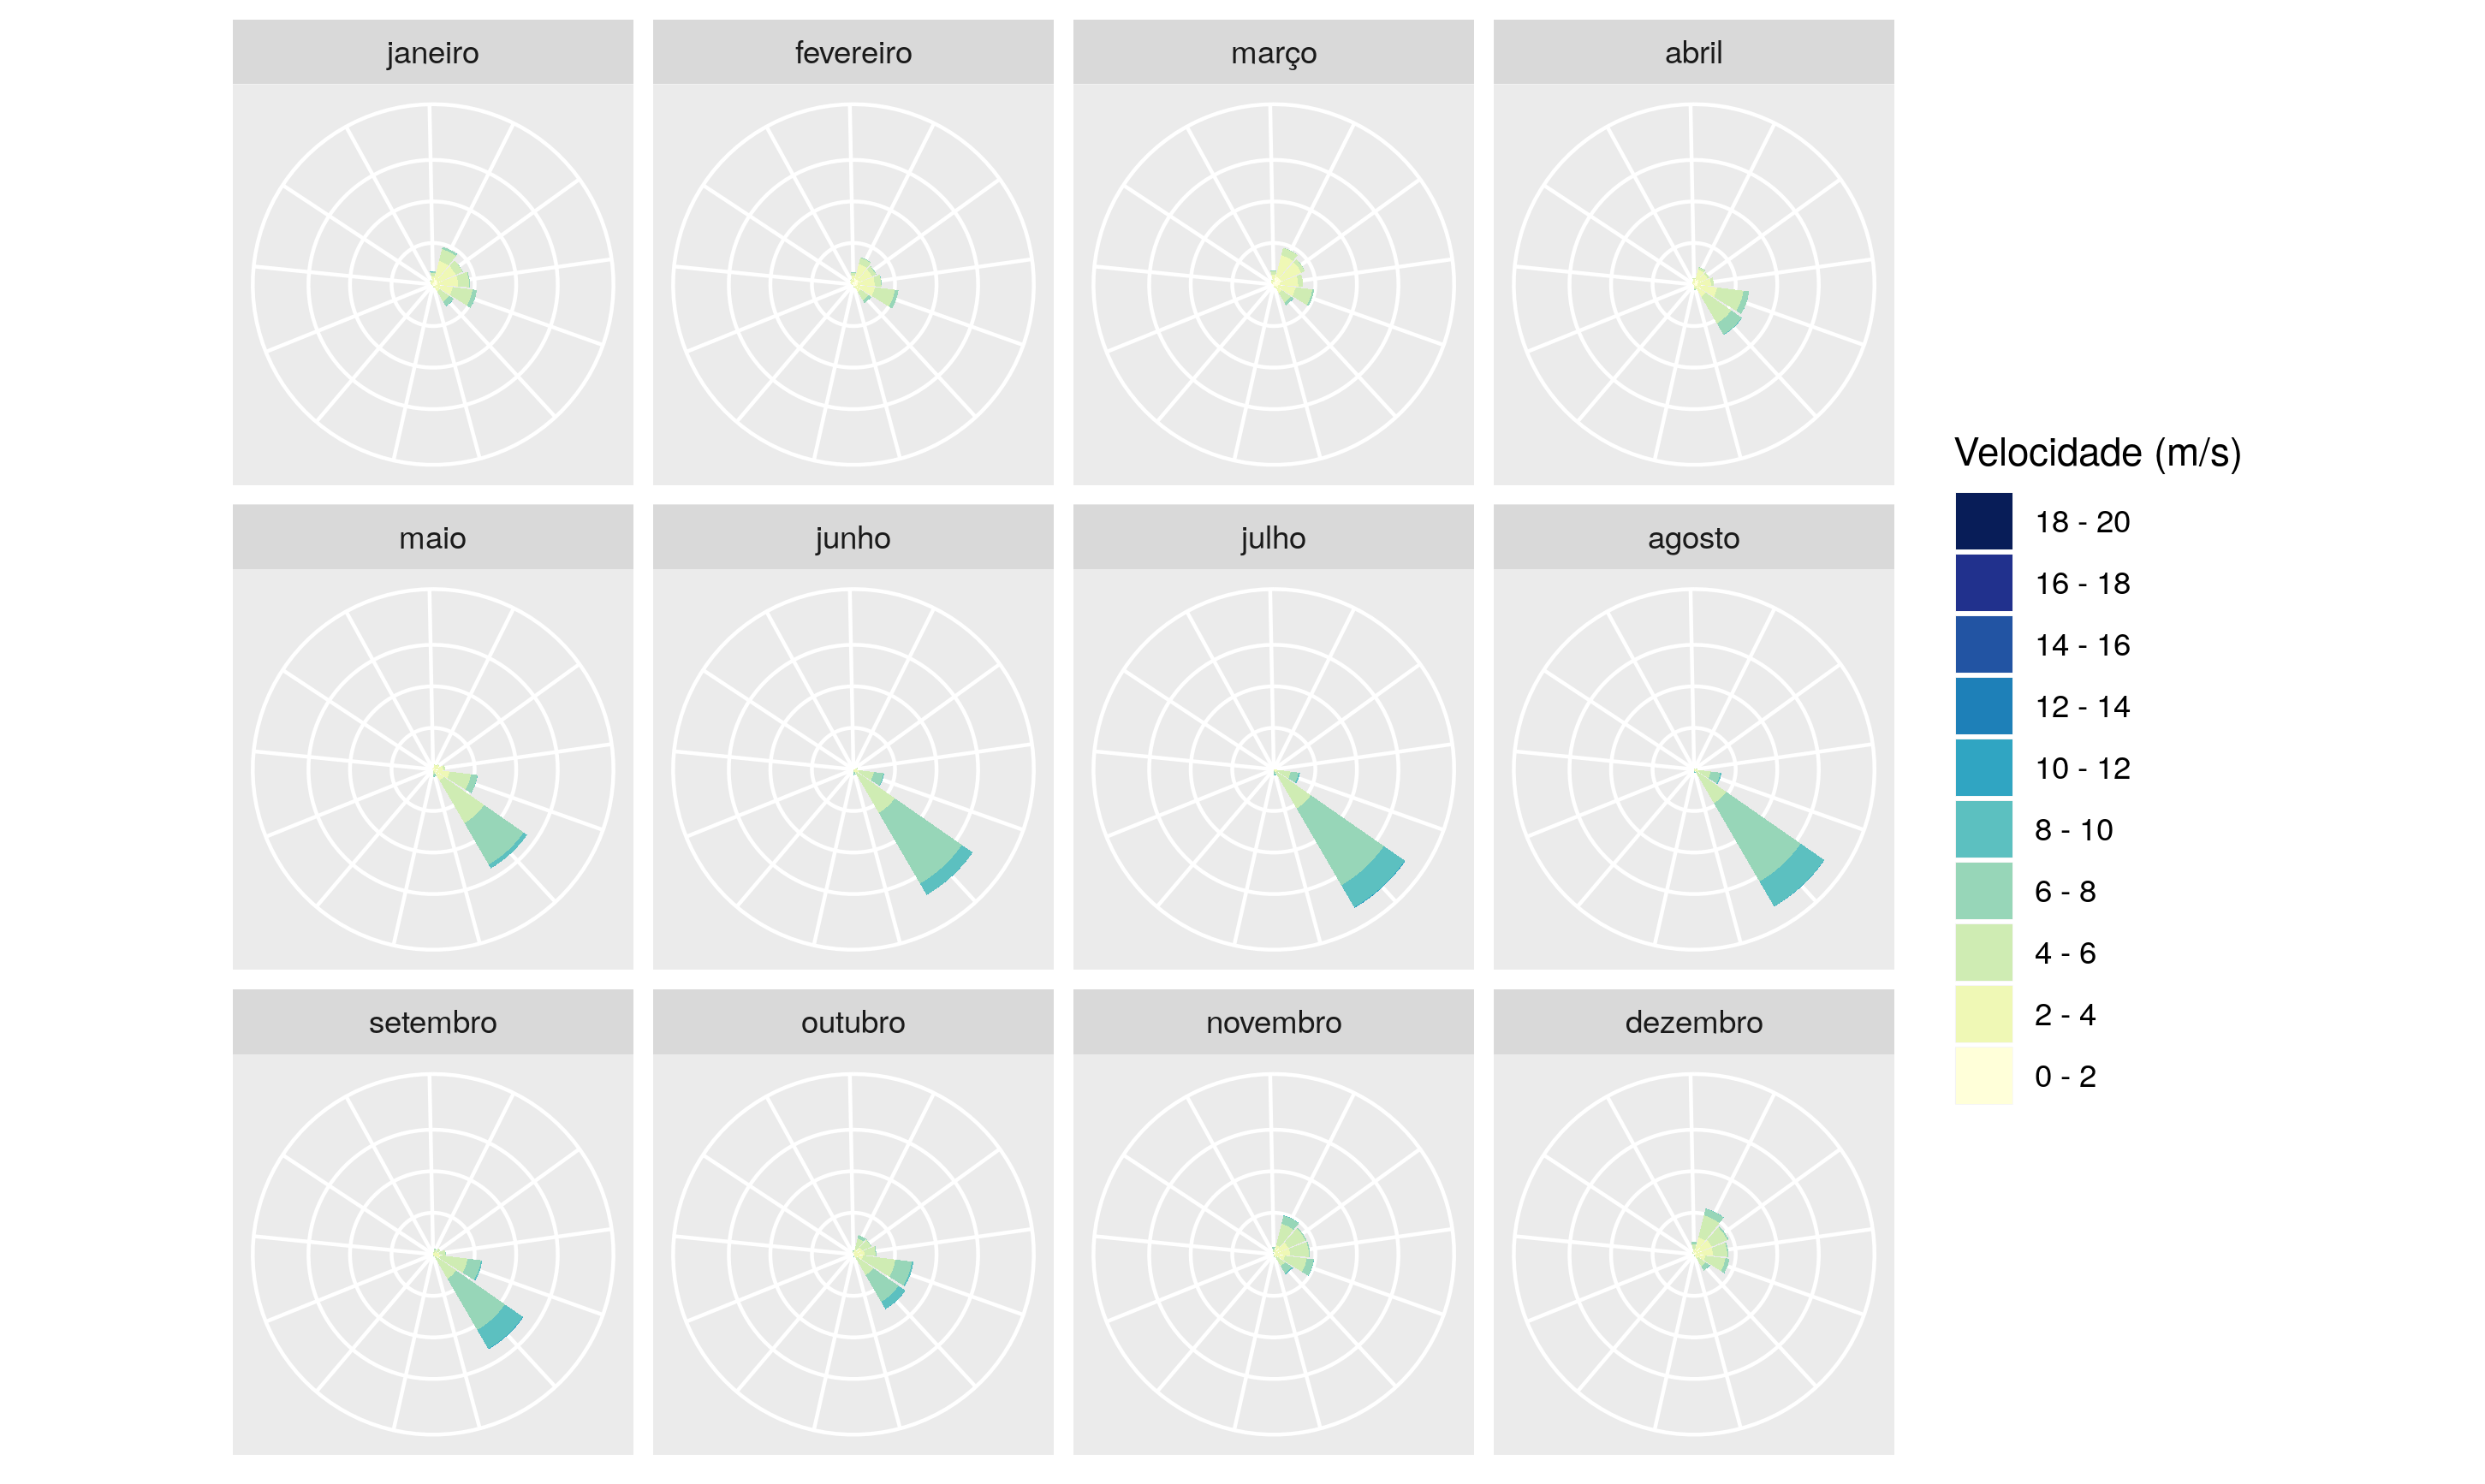
\includegraphics[scale=0.55]{windrose_monthly}
%%%		\caption{Rosas dos ventos mensais do recurso eólico da cidade de Sento Sé. Fonte: autoria própria, dados: ECWMF.}
%	\end{figure}
%}

%\begin{frame}
%	\frametitle{O Jogo do Caos}
%	\begin{columns}[t]
%		\column{.5\textwidth}
%		\centering
%		\fbox{\includegraphics[scale=0.5]{first}}\\
%		\vspace{0.5cm}
%		\fbox{\includegraphics[scale=0.5]{third}}\\
%		\column{.5\textwidth}
%		\centering
%		\vspace{0.5cm}
%		\fbox{\includegraphics[scale=0.5]{second}}
%		\fbox{\includegraphics[scale=0.5]{last}}
%	\end{columns}
%
%	\vspace{0.5cm}
%	O Jogo do Caos. Fonte: Wikimedia Commons. CC BY-SA 3.0
%\end{frame}

%\frame
%{
%	\frametitle{Triângulo de Sierpinski}
%	\begin{figure}[h]
%    	\centering
%		\includegraphics[scale=0.2]{triangle}
%%%		\caption{Triângulo de Sierpinski. Fonte: Wikimedia Commons. CC BY-SA 3.0}
%	\end{figure}
%}

%\frame
%{
%	\frametitle{O caráter estocástico do vento: anual}
%	\begin{figure}[h]
%	    \centering
%		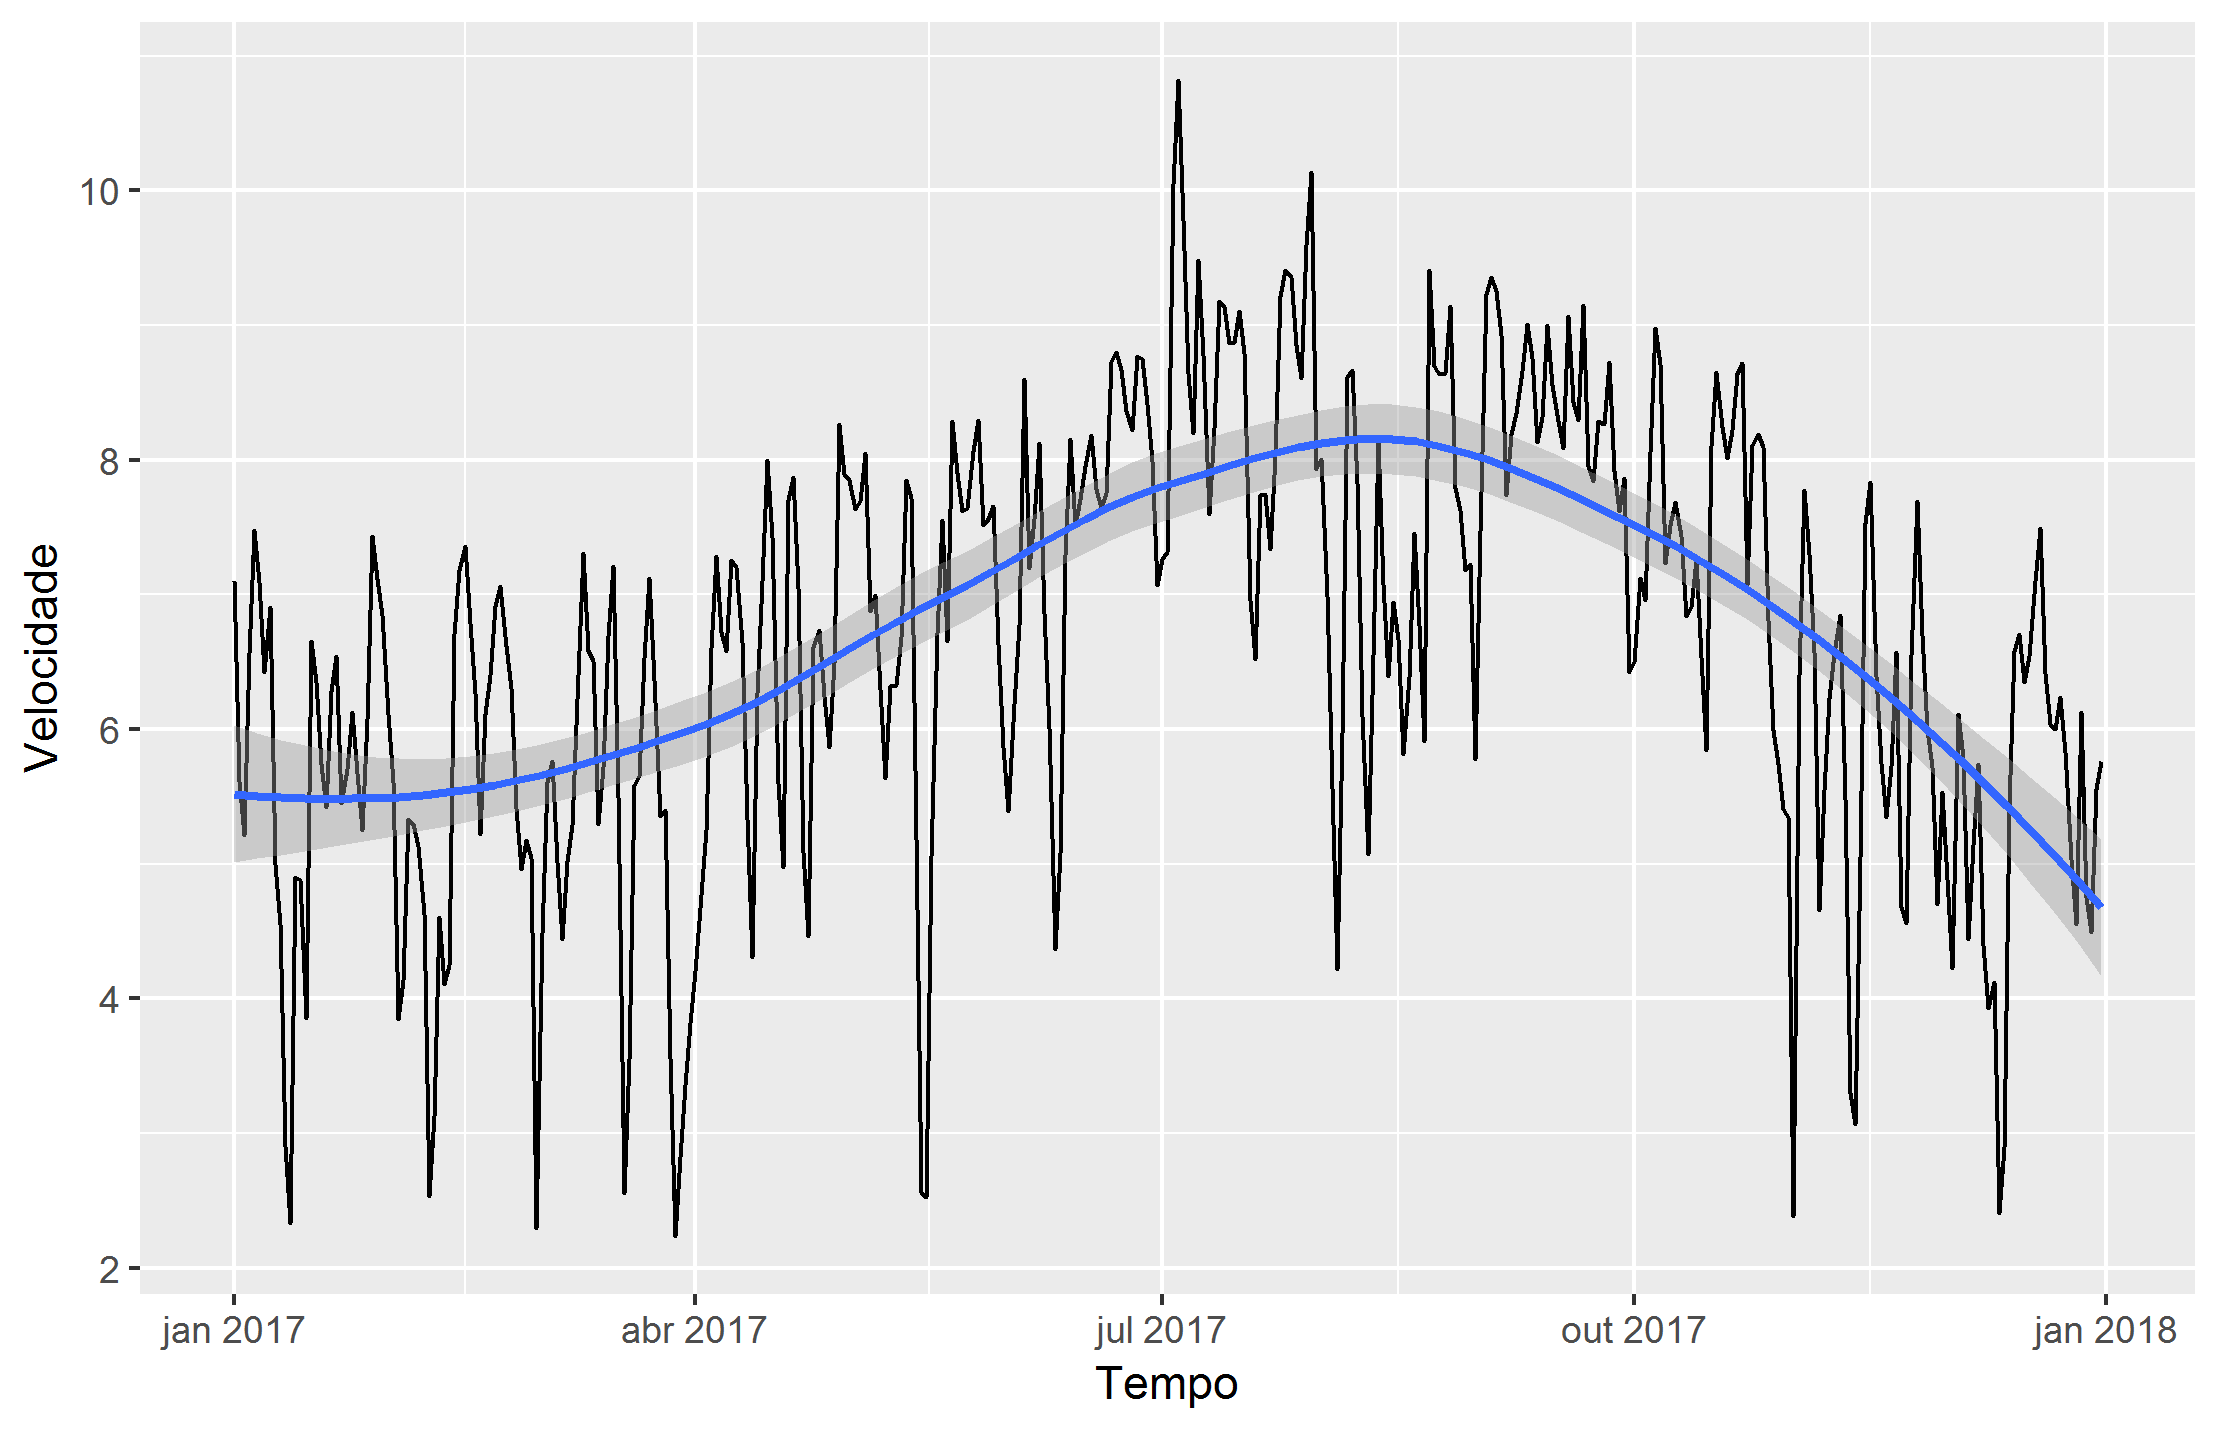
\includegraphics[scale=0.55]{stochastic}
%%%		\caption{Velocidade do vento medida por satélite na cidade de Sento Sé. Fonte: autoria própria. Dados: ECWMF. Curva em azul: ajuste aos dados medidos, dados: ECMWF}
%	\end{figure}
%}

%\frame
%{
%	\frametitle{O caráter estocástico do vento: mensal}
%	\begin{figure}[h]
%    	\centering
%		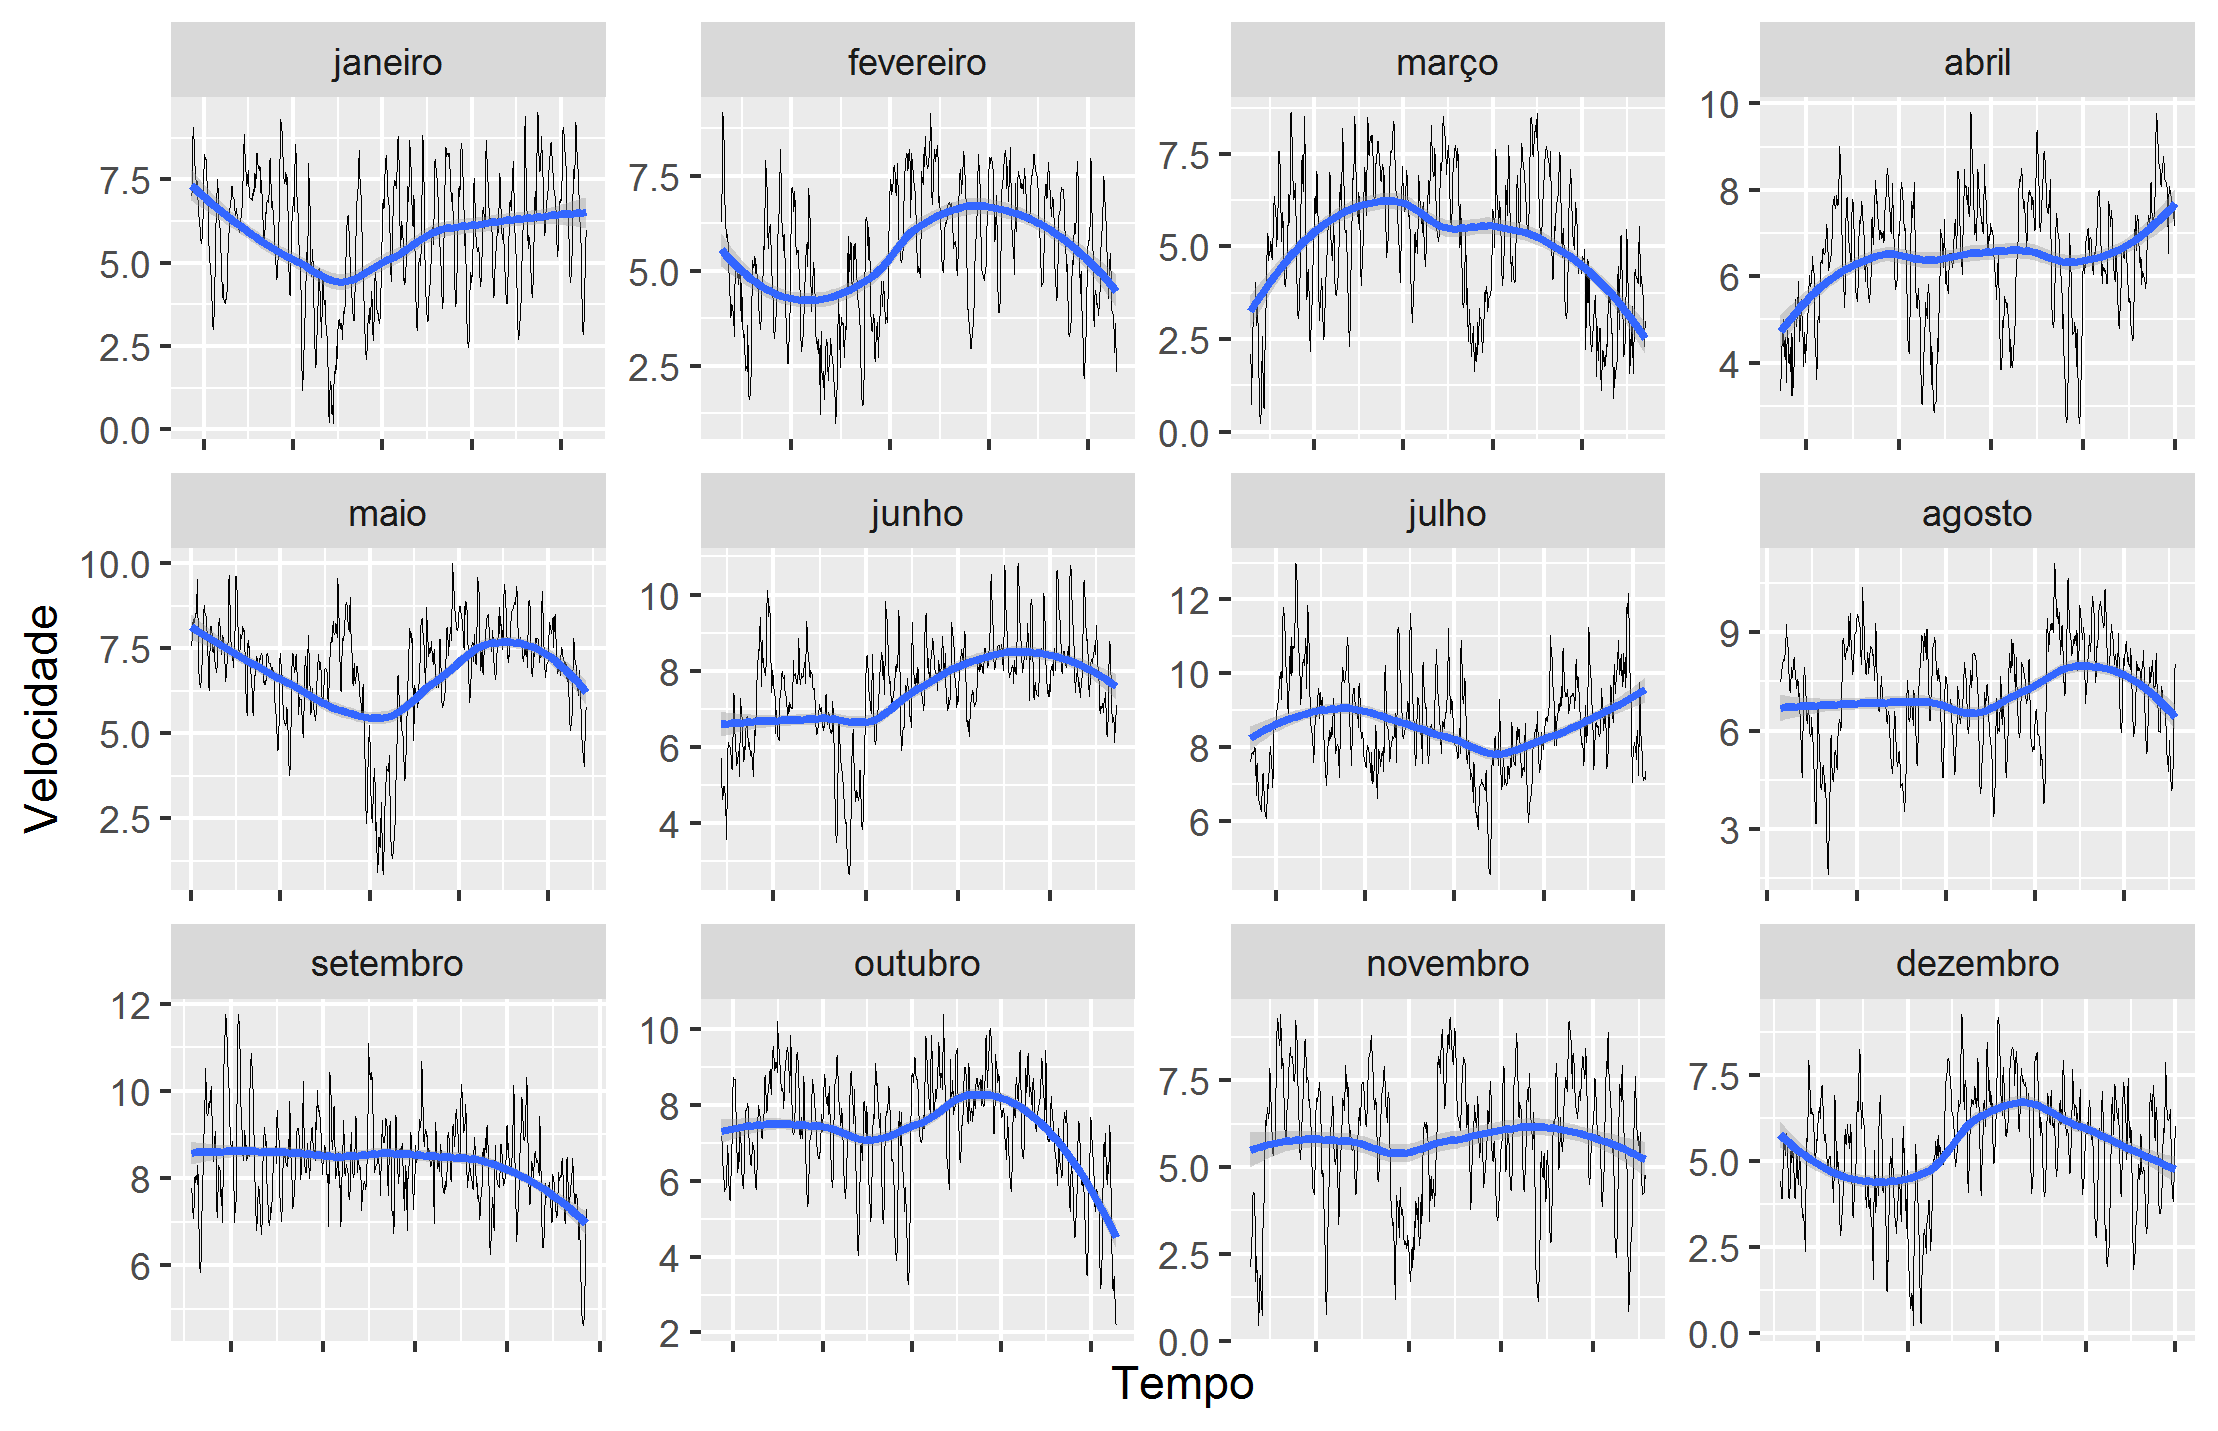
\includegraphics[scale=0.53]{stochastic_monthly}
%%%		\caption{Velocidade do vento para cada mês do ano de 2017 da cidade de Sento Sé no norte da Bahia. Curva em preto: dados medidos. Curva em azul: ajuste aos dados medidos. Fonte: autoria própria, dados: ECMWF.}
%	\end{figure}
%}

%\frame
%{
%	\frametitle{Ordem em meio ao caos}
%	\begin{figure}[h]
%	    \centering
%		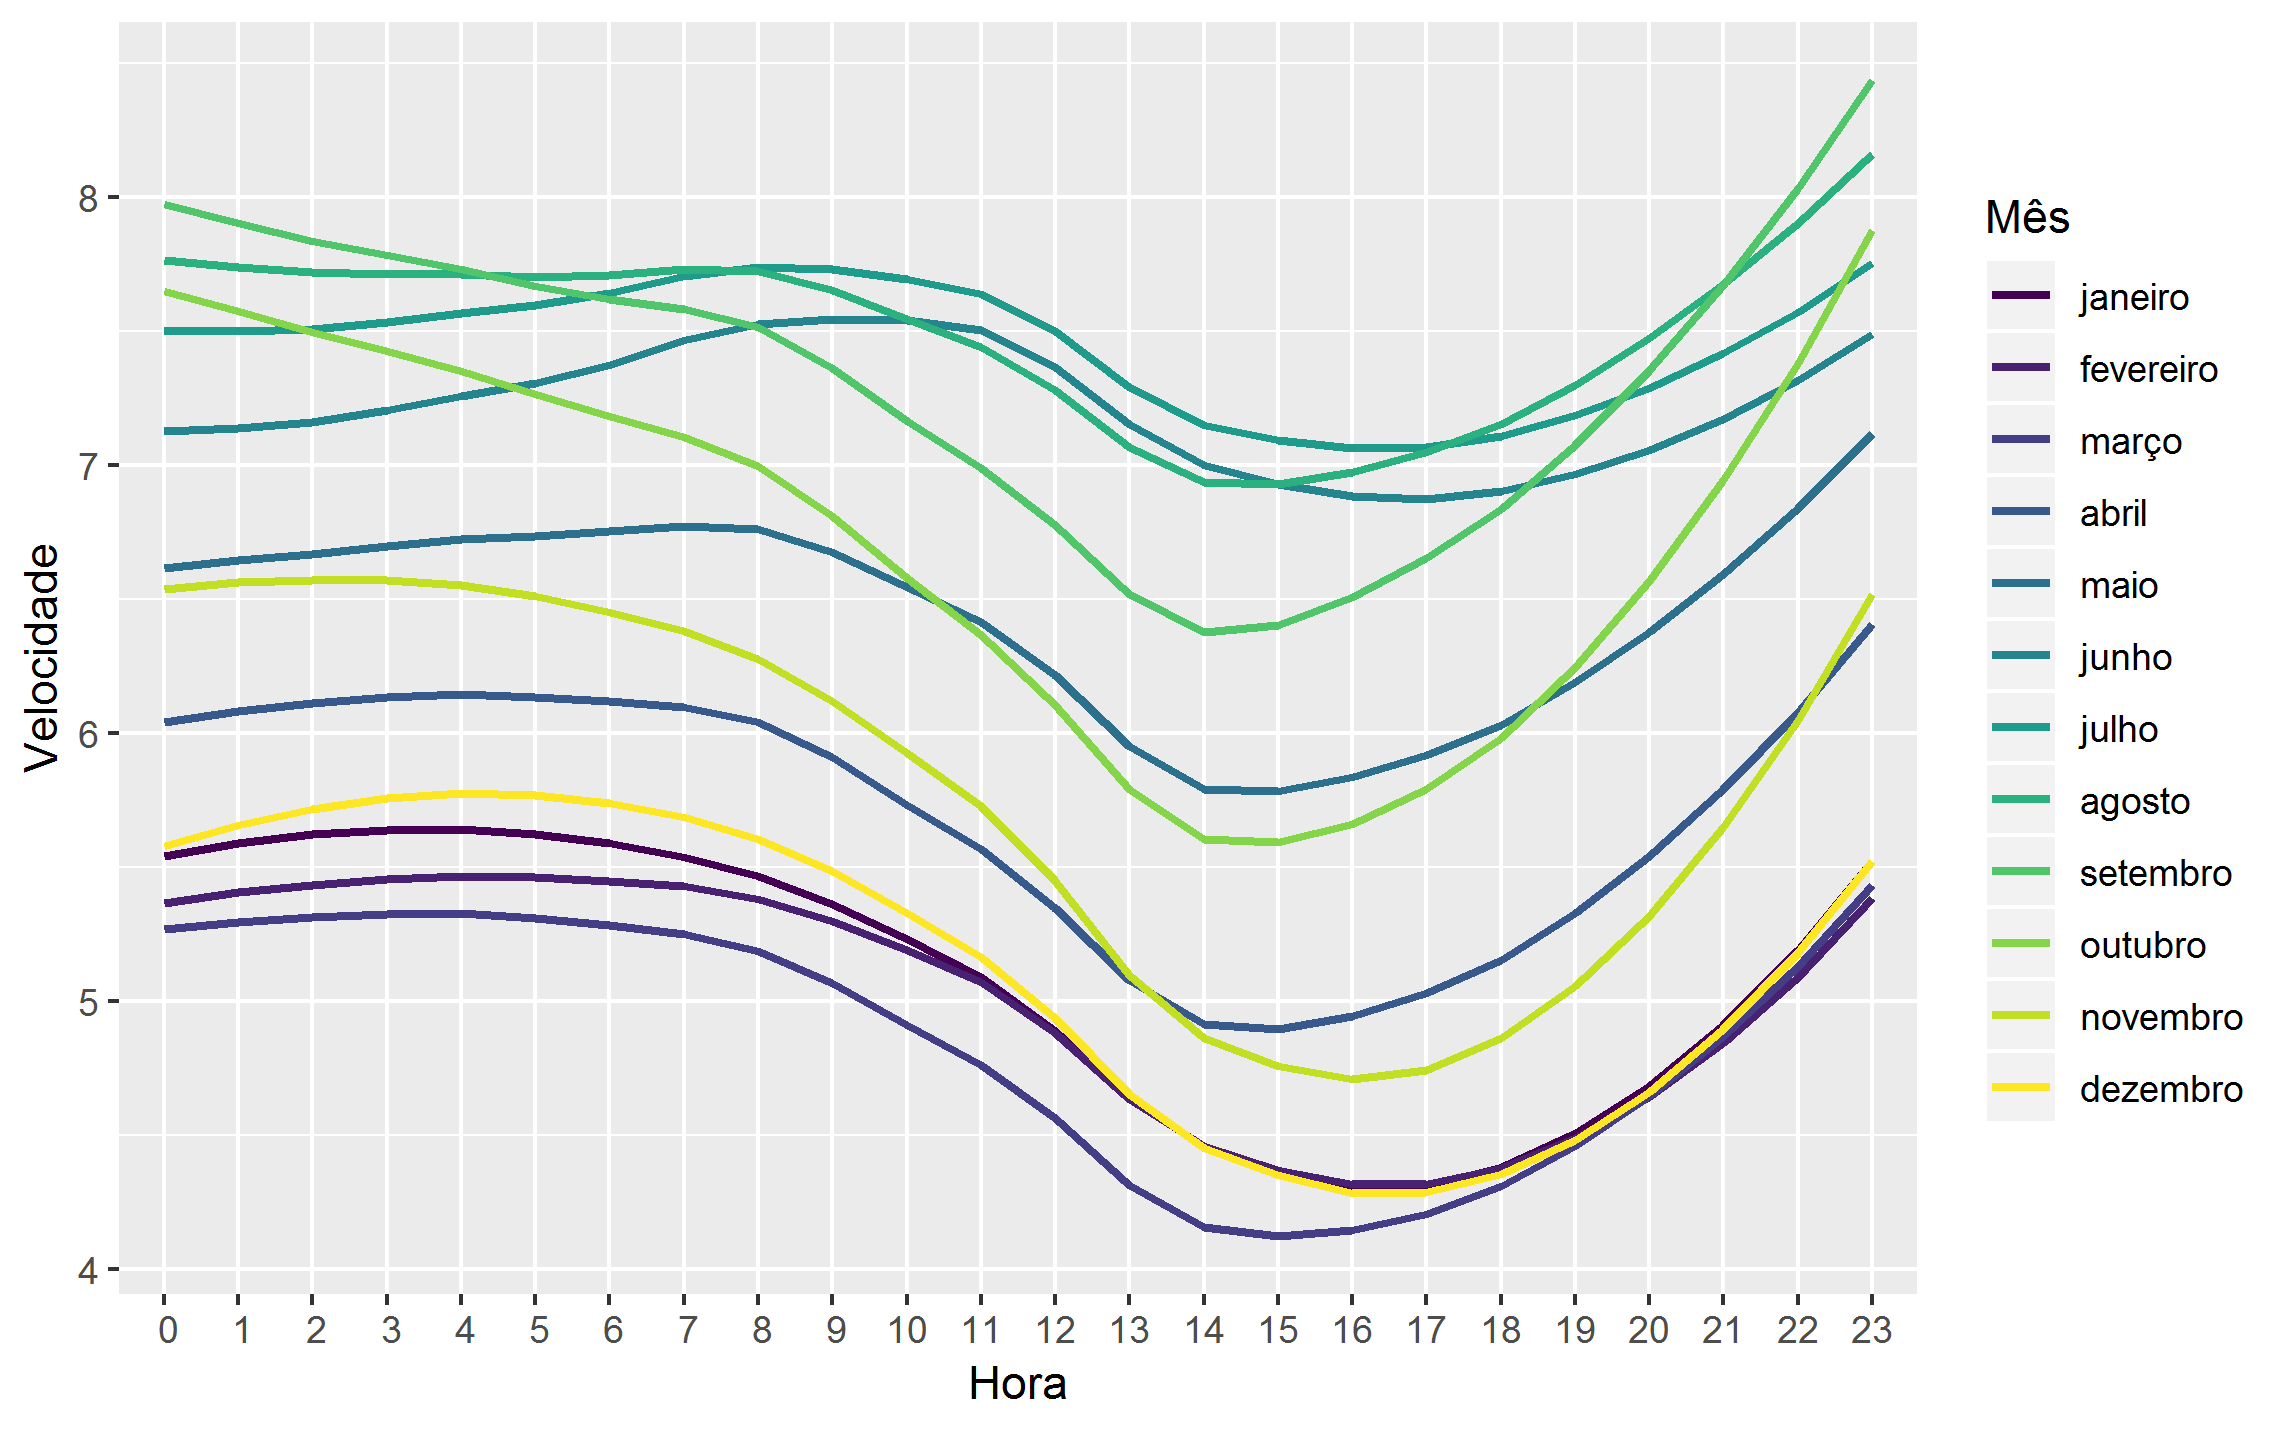
\includegraphics[width=\textwidth]{diurnal}
%%%		\caption{Velocidade do vento para cada hora do dia e para cada mês do ano de 2017. Fonte: autoria própria, dados: ECWMF.}
%	\end{figure}
%}

%\frame
%{
%	\frametitle{Precisão numérica}
%	\begin{figure}[h]
%    	\centering
%		\includegraphics[scale=0.8]{grid}
%%%		\caption{Grid de medições. Fonte: Earth Magazine.}
%	\end{figure}
%}

%\frame
%{
%	\frametitle{Recurso eólico de longo prazo: distribuição de Weibull}
%	\begin{figure}[h]
%	    \centering
%		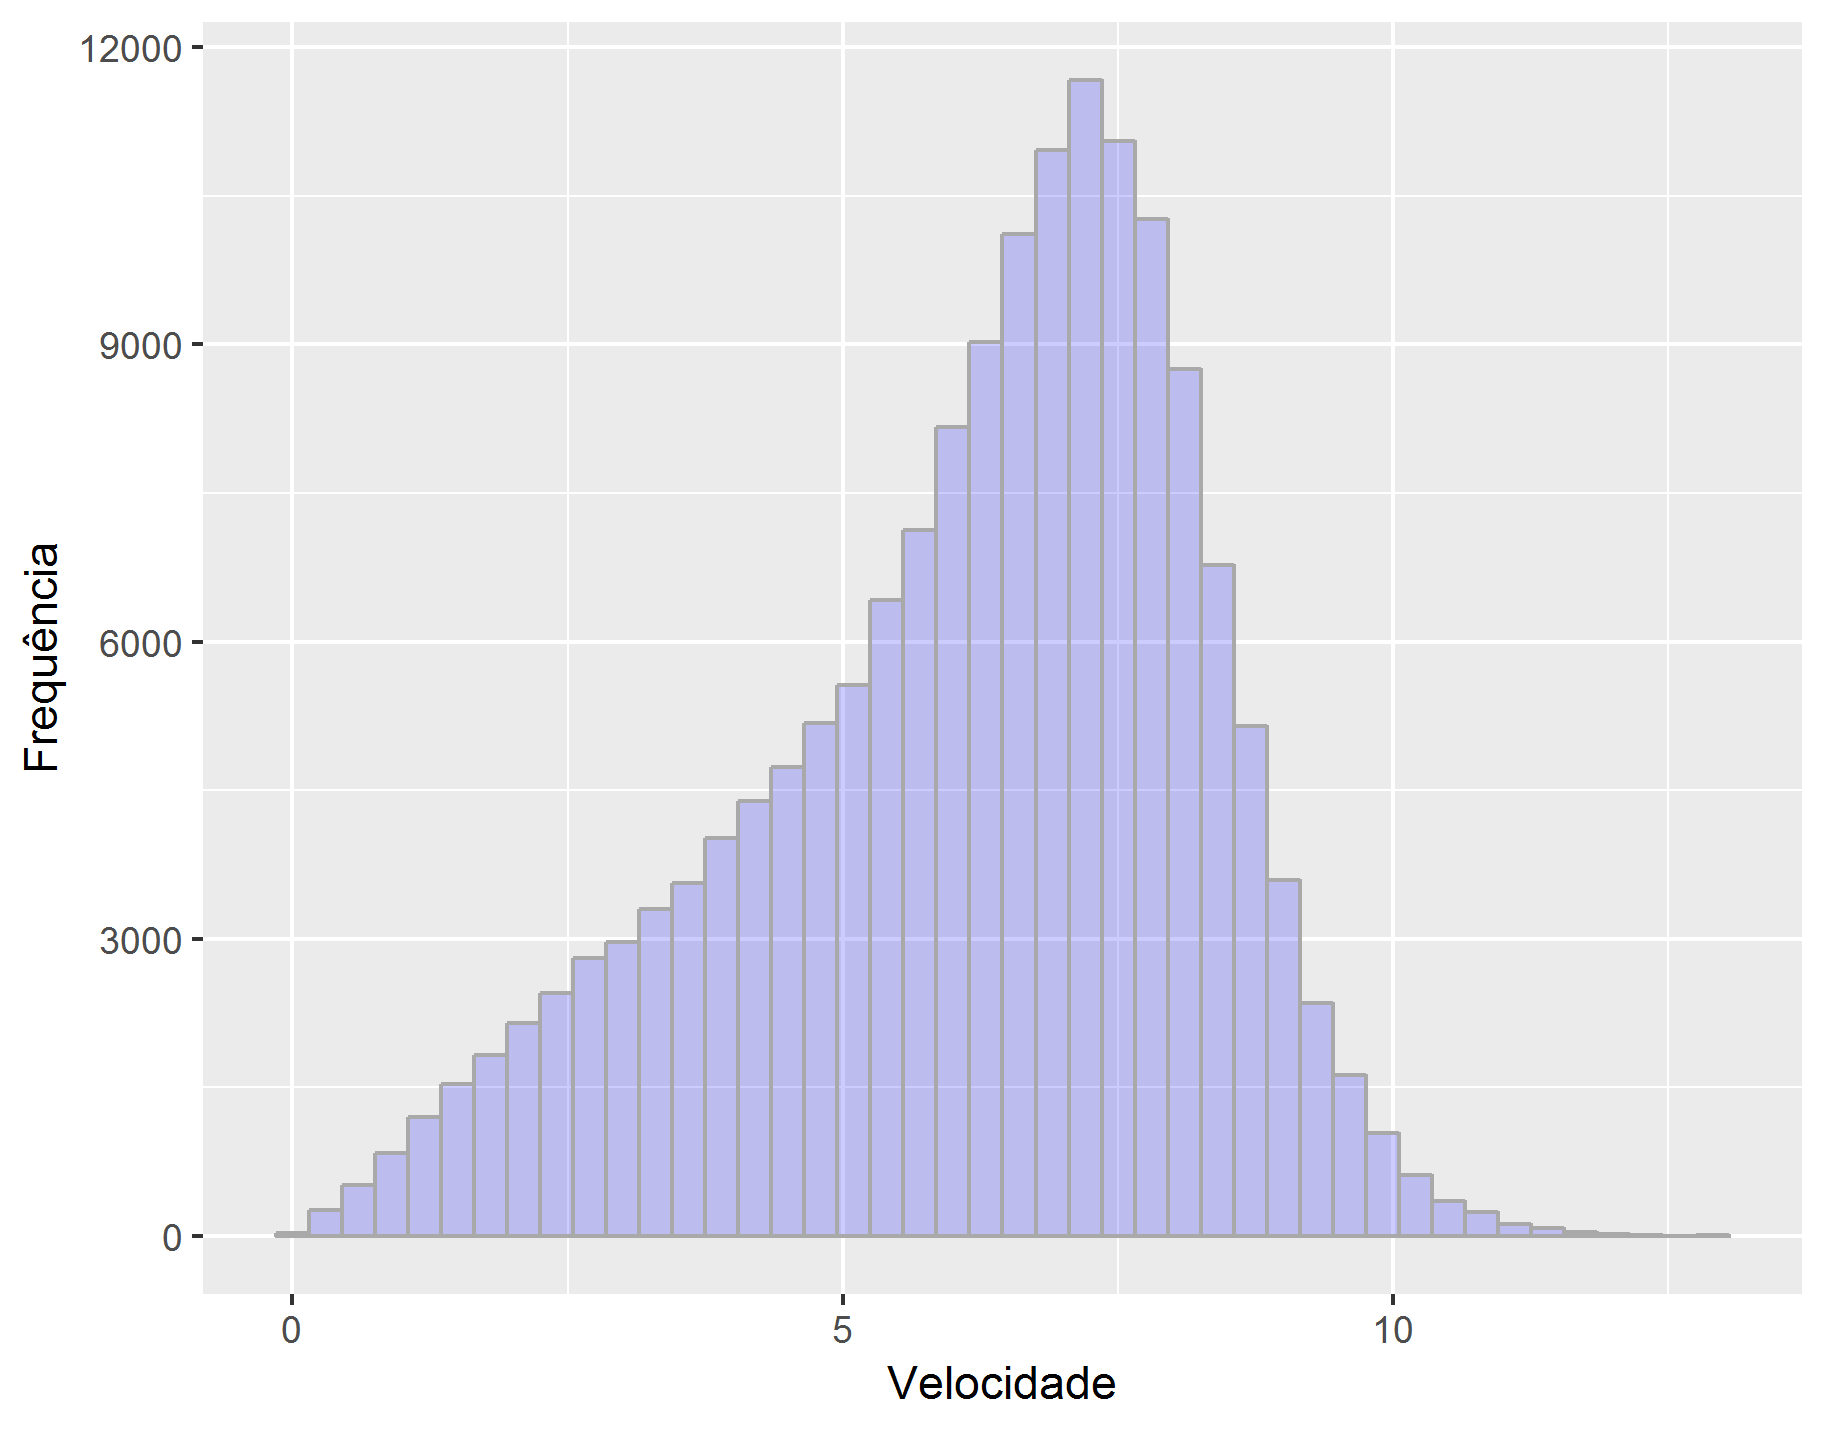
\includegraphics[scale=0.55]{weibull_histogram}
%%%		\caption{A distribuição de velocidades do quadrante central. Fonte: autoria própria, dados: ECWMF.}
%	\end{figure}
%}

%\frame
%{
%	\frametitle{Recurso eólico de longo prazo: distribuição de Weibull}
%	\begin{figure}[h]
%	    \centering
%		\includegraphics[scale=0.55]{weibull_freqpoly}
%%%		\caption{Distribuição de velocidades de todos os quadrantes. Fonte: autoria própria, dados: ECWMF.}
%	\end{figure}
%}

%\frame
%{
%    \frametitle{Resolução temporal}
%	Estimativa do recurso eólico em base mensal, diária, horária?
%	\begin{itemize}
%		\item 	mensal: negociação mais sólida com investidores
%		\item 	diária: minimizar perdas por manutenção
%		\item 	horária: adequamento da oferta de energia ao consumo local
%	\end{itemize}
%}

%\frame
%{
%	\frametitle{O cálculo estocástico na economia}
%	\begin{figure}[h]
%	    \centering
%		\includegraphics[scale=0.45]{stock}
%%%		\caption{Valor de abertura das ações da Google na NASDAQ. Curva em preto: dados medidos. Curva em azul: curva ajustada aos dados medidos. Fonte: autoria própria, dados: Google Finance.}
%	\end{figure}
%}

%\frame
%{
%	\frametitle{Proposta do trabalho}
%	\begin{block}{Objetivo}
%		Estimar a produção de energia, a partir de dados de vento, em curtos intervalos de tempo por meio de um modelo que contemple o caráter estocástico, físico, real do vento.
%	\end{block}
%}

%\frame
%{
%	\frametitle{Proposta do trabalho}
%	Para cumprir a proposta do trabalho é preciso:
%	\begin{itemize}
%		\item Fazer uma revisão da literatura
%		\item Entender fundamentos matemáticos: cálculo de Ito, teoria do caos, Monte Carlo
%		\item Entender os limites do estudo (precisão numérica, horizonte de previsão)
%		\item Simulação numérica
%		\item Entender como a estimativa de energia (de 20 anos) é feita
%		\item Comparação entre métodos e com dados medidos
%	\end{itemize}
%}

%\frame
%{
%	\frametitle{Planejamento}
%	\begin{figure}[h]
%		\hspace*{-0.8cm}   
%    	\includegraphics[scale=0.41]{gantt}
%	    \caption{Gráfico de Gantt do planejamento das etapas de desenvolvimento do presente trabalho. Fonte: autoria própria.}
%    	\centering
%	\end{figure}
%}

\end{document}
